 %
% To start the document, use
%  \levela{...}
% For lover level, sections use
%  \levelb{...}
%  \levelc{...}
%
\levela{Gas Absorption}
 \label{sec:absorption}


%
% Document history, format:
%  \starthistory
%    date1 & text .... \\
%    date2 & text .... \\
%    ....
%  \stophistory
%
\starthistory
  2001-07-05 & Template created by Stefan Buehler.\\
  2001-10-05 & Line absorption part written, Nikolay Koulev\\
  2001-11-21 & Continuum absorption part written, Thomas Kuhn.\\
\stophistory
%
% Symbol table, format:
%  \startsymbols
%    ... & \verb|...| & text ... \\
%    ... & \verb|...| & text ... \\
%    ....
%  \stopsymbols
%
%
%\startsymbols
%  -- & -- & -- \\
% \label{symtable:wfuns}     
%\stopsymbols

% ============================================================================

% ============================================================================
% TKS definitions for the sections "Continuum Absorption" and 
% "Complete Absorption Models"
%
\def\deni{\rho_{\mbox{\rm i}}}
\def\denl{\rho_{\mbox{\rm l}}}
\def\denli{\rho_{\mbox{\rm l,i}}}
%
\def\imn{{N''}}
\def\ime{\epsilon^{''}_r}
\def\ree{\epsilon^{'}_r}
\def\er{\epsilon_r}
%
\def\bek{\rm b_{\rm 1,k}}
\def\bzk{\rm b_{\rm 2,k}}
\def\bdk{\rm b_{\rm 3,k}}
\def\bvk{\rm b_{\rm 4,k}}
\def\bfk{\rm b_{\rm 5,k}}
\def\bsk{\rm b_{\rm 6,k}}
%
\def\bekp{\rm \widehat{b}_{\rm 1,k}}
\def\bzkp{\rm \widehat{b}_{\rm 2,k}}
\def\bdkp{\rm \widehat{b}_{\rm 3,k}}
\def\bvkp{\rm \widehat{b}_{\rm 4,k}}
\def\bfkp{\rm \widehat{b}_{\rm 5,k}}
\def\bskp{\rm \widehat{b}_{\rm 6,k}}
%
\def\beks{\rm b^*_{\rm 1}}
\def\bzks{\rm b^*_{\rm 2}}
\def\bdks{\rm b^*_{\rm 3}}
\def\bvks{\rm b^*_{\rm 4}}
\def\bfks{\rm b^*_{\rm 5}}
\def\bsks{\rm b^*_{\rm 6}}
%
\def\bekps{\rm \widehat{b^*}_{\rm 1,k}}
\def\bzkps{\rm \widehat{b^*}_{\rm 2,k}}
\def\bdkps{\rm \widehat{b^*}_{\rm 3,k}}
\def\bvkps{\rm \widehat{b^*}_{\rm 4,k}}
\def\bfkps{\rm \widehat{b^*}_{\rm 5,k}}
\def\bskps{\rm \widehat{b^*}_{\rm 6,k}}
%
\def\air{\mbox{air}}
\def\am{\mbox{NH}_3}
\def\hzo{\mbox{H}_2\mbox{O}}
\def\nzo{\mbox{N}_2\mbox{O}}
\def\nz{\mbox{N}_2}
\def\oz{\mbox{O}_2}
\def\co{\mbox{CO}}
\def\coz{\mbox{CO}_2}
\def\clo{\mbox{ClO}}
%
\def\vmroz{VMR_{\mbox{\rm \small O}_{2}}}
%
\def\ptot{P_{\mbox{\rm \small tot}}}
\def\phzo{P_{\mbox{\rm \small H2O}}}
\def\pnz{P_{\mbox{\rm \small N2}}}
\def\poz{P_{\mbox{\rm \small O2}}}
\def\pda{P_{\mbox{\rm \small d}}}
\def\pdair{P_{\mbox{\rm \small air}}}
\def\pan{P_{\mbox{\rm \small air,N2}}}
\def\pcoz{P_{\mbox{\rm \small CO2}}}
%
\def\alphatot{\alpha_{\mbox{\rm \small tot}}} 
\def\alphal{\alpha_{\ell}} 
\def\alphac{\alpha_{\mbox{\small c}}}
\def\alphacs{\alpha_{\mbox{\rm \small c,s}}} 
\def\alphacf{\alpha_{\mbox{\rm \small c,f}}}
%
\def\alphampmotot{\alpha^{\mbox{\rm \small MPM87}}_{\mbox{\small tot}}} 
\def\alphampmmtot{\alpha^{\mbox{\rm \small MPM89}}_{\mbox{\small tot}}} 
\def\alphampmntot{\alpha^{\mbox{\rm \small MPM93}}_{\mbox{\small tot}}} 
\def\alphapwrtot{\alpha^{\mbox{\rm \small R98}}_{\mbox{\small tot}}} 
\def\alphacptot{\alpha^{\mbox{\rm \small CP98}}_{\mbox{\small tot}}} 
%
\def\alphampmol{\alpha^{\mbox{\rm \small MPM87}}_{\mbox{\small $\ell$}}} 
\def\alphampmml{\alpha^{\mbox{\rm \small MPM89}}_{\mbox{\small $\ell$}}} 
\def\alphampmnl{\alpha^{\mbox{\rm \small MPM93}}_{\mbox{\small $\ell$}}} 
\def\alphampml{\alpha^{\mbox{\rm \small MPM}}_{\mbox{\small $\ell$}}} 
\def\alphapwrl{\alpha^{\mbox{\rm \small R98}}_{\mbox{\small $\ell$}}} 
\def\alphacpl{\alpha^{\mbox{\rm \small CP98}}_{\mbox{\small $\ell$}}} 
%
\def\alphampmoc{\alpha^{\mbox{\rm \small MPM87}}_{\rm c}} 
\def\alphampmmc{\alpha^{\mbox{\rm \small MPM89}}_{\rm c}} 
\def\alphampmnc{\alpha^{\mbox{\rm \small MPM93}}_{\rm c}} 
\def\alphapwrc{\alpha^{\mbox{\rm \small R98}}_{\rm c}} 
\def\alphacpc{\alpha^{\mbox{\rm \small CP98}}_{\rm c}} 
%
\def\gamk{\gamma_{\mbox{\rm \small k}}}
\def\gamc{\gamma_{\mbox{\rm \small c}}}
%
\def\ws{w_{\mbox{\rm \small s,k}}}
\def\xs{x_{\mbox{\rm \small s,k}}}
\def\wf{w_{\mbox{\rm \small f,k}}}
\def\xf{x_{\mbox{\rm \small f,k}}}
%
\def\wn{\bar{\nu}}
\def\nucc{\nu_{\mbox{\rm \small c}}}
\def\nucut{\nu_{\mbox{\rm \small cutoff}}}
\def\nuo{\nu_{\mbox{\rm \small 0}}}
\def\nuk{\nu_{\mbox{\rm \small k}}}
%
\def\shape{F(\nu,\nuk)}
\def\shapec{F_{c}(\nu,\nuk)}
\def\shapefp{f_{c}(\nu,+\nuk)}
\def\shapefm{f_{c}(\nu,-\nuk)}
\def\shapefpm{f_{c}(\nu,\pm\nuk)}
\def\inten{S_{\mbox{\rm \small k}}(T)}
\def\inteno{S_{\mbox{\rm \small k}}(300\,K)}
\def\intencp{S_{\mbox{\rm \small 0}}(T)}
%
\def\cx{C_{\mbox{\rm \small x}}}
\def\cs{C_{\mbox{\rm \small H}_{2}\mbox{\rm \small O}}} 
\def\cf{C_{\mbox{\rm N}_{2}}} 
\def\cxo{C^{\mbox{\rm o}}_{\mbox{\rm \small X}}} 
\def\cso{C^{\mbox{\rm o}}_{\mbox{\rm \small H}_{2}\mbox{\rm \small O}}} 
\def\cfo{C^{\mbox{\rm o}}_{\mbox{\rm \small N}_{2}}} 
\def\cao{C^{\mbox{\rm o}}_{\mbox{\rm \small air}}}
\def\cdo{C^{\mbox{\rm o}}_{\mbox{\rm \small d}}}
\def\xx{{\rm n}_{\mbox{\rm \small  x}}} 
\def\xs{{\rm n}_{\mbox{\rm \small  s}}} 
\def\xf{{\rm n}_{\mbox{\rm \small  f}}} 
\def\xd{{\rm n}_{\mbox{\rm \small  d}}}
%
% ============================================================================


                                          

In general there are three types of absorption/emission spectra:
\begin{itemize}
\item sharp lines of finite width
\item aggregations (series) of lines called bands
\item continua extending over a broad range of wavelengths, with
      no single lines in it.
\end{itemize}
This section is therefore firstly devised to give a short theoretical
overview of the absorption quantities which are used in ARTS. The
presentation of the calculation methods within ARTS of these
quantities is the second goal. There are two major subsections which
deal separately with the respective types of spectra regarded by ARTS,
lines and continua.  The second one extends beyond the scope of mere
treatment of the continua and thus gives an integrated view of
continua and spectral lines.

% ================================================================================
% The following section is written by Nikolay Koulev, iup Bremen, nkoulev@uni-bremen.de
% ================================================================================

\levelb{Line Absorption}
%-----------------------
\label{sec:line_absorption}

 
We will introduce here the main concepts concerning
line absorption. The approach, however, does not aim  at the
derivation, but rather at the presentation the following expressions.

Any line is presented by the corresponding profile of the absorption/emission
coefficient as a function of the frequency, in our case that of the
absorption - given by the quantity $\alpha(\nu)$. The latter dependency
is related to other quantities, which express the three
characteristics of a single line uniquely describing it - position,
strength and shape. 
The strength, or better the line intensity, is given by the quantity
$S(T)$, where $T$ is absolute temperature. The shape and the position are expressed through the
line-shape function $F(\nu)$. Thus we have the relation    
\begin{equation}\label{abs_coeff}
  \alpha(\nu)=nS(T)F(\nu)
\end{equation} 
where $n$ is the number density of the absorber, \citet{goodyandyung:89}. The line-shape
function is normalized as follows

\begin{equation}\label{line_shape_norm}
  \int F(\nu)d\nu=1
\end{equation}
The values of $S(T)$ at reference temperature $T_0$ are contained in
spectroscopic databases. The conversion to different temperatures is
done by
\begin{equation}\label{line_intensity}
  S(T)=S(T_0)~\frac{Q(T_0)}{Q(T)}~\frac{e^{-E_f/(kT)}
    - e^{-E_i/(kT)}}{e^{-E_f/(kT_0)} - e^{-E_i/(kT_0)}}
\end{equation}
given the energies $E_f$ and $E_i$ of the two levels between which the
transition occurs as well as the partition function~~$Q(T)$, \citet{rothman:98}. The
databases contain the lower state energy $E_l$ tabulated along with
the $S$ and the transition frequency $\nu$, so that the upper state
energy can be computed by $E_u$=$E_l$+h$\nu$. Partition functions for
all molecular species are also available along with spectroscopic
databases, either in the form of tabulated values for a set
temperatures, or in the form of FORTRAN routines. One can obtain the
total absorption coefficient by adding the absorption of all spectral
lines of all molecular species.

The problem of determining the explicit kind of the line-shape
functions is treated in the following subsection. Another one is
dedicated to the partition functions and their calculation..


\levelc{Line Shape Functions} Up to date there is no way to calculate
the line-shape functions analytically just from the theoretical
expressions of quantum dynamics, statistical physics, and theoretical
mechanics. Certain approximations have to be made to account for
different physical phenomena related to the absorption/emission
process or to suit better the calculation of different parts of the
spectral line.

There are three phenomena which contribute to the line-shape. These
are, in increasing order of importance, the finite lifetime of an
excited state in an isolated molecule, the thermal movement of the gas
molecules, and their collisions with each other. They result in
corresponding effects to the line-shape: natural broadening, Doppler,
and pressure broadening. Of these, the first one is completely
negligible compared to the other two. Nevertheless, we will pay a
special attention to the natural broadening because its implications
are of a conceptual importance for the broadening processes.

The spectral line shape can be derived in the case of natural
broadening from basic physical considerations and a well-known Fourier
transform theorem from the time to the frequency domain, \citet{thorne:99}. If we
consider classically the spontaneous decay of the excited state of
two-level system in the absence of external radiation, then population
$n$ of these level decreases according to
\begin{equation}\label{spon_decay_diff}
  \frac{dn(t)}{dt} = -A\,n(t)
\end{equation}
where $A$ is Einstein A coefficient, which equation can also be
interpreted as the rate of the spontaneously emitted photons because
of decay. This relation is more usefully in this case to be written in
the following manner 
\begin{equation}\label{spon_decay_exp}
  n(t)=n(0)~e^{-At}=n(0)e^{-t/\tau}
\end{equation}
where $ \tau$ is the mean lifetime of the excited state. Thus the
number of spontaneously emitted photons and in this way the flux of
the emitted radiation then will be proportional to $n$. Therefore we
can write for the flux $L$ that
\begin{equation}\label{flux}
  L(t)=L(0)~e^{-t/ \tau}=L(0)~e^{-\gamma t}
\end{equation}
By the afore mentioned theorem, multiplying in the time domain by
$e^{-\gamma t}$ is equivalent to convolving in the frequency domain
with a function $1/[\nu^2 - (\gamma/4\pi)^2]$. Accordingly the line
profile of a spectral line at frequency $ \nu_0$ as a normalized
line-shape function will be, as difined in \citet{thorne:99},
\begin{equation}\label{natural_lorentz}
  F(\nu)=\frac{1}{\pi}\frac{\gamma/4\pi}{(\nu - \nu_0)^2 + (\gamma/4\pi)^2}
\end{equation}
This gives a bell-shaped profile and the function itself is called
Lorentzian. The dependence on the position of the line is apparent
through $\nu_0$, that is why some authors prefer to denote the
function by $F(\nu,\nu_0)$.  The result is important because of two
major reasons.  Firstly, without the natural broadening the line would
be the delta function~$\delta (\nu - \nu_o)$, as pointed out in
\citet{bernath:95}. So the spontaneous decay of the excited state is
responsible for the finite width and the certain shape of the
line-shape function. Secondly, the Lorentzian type of function comes
significantly into play when explaining some of the other broadening
effects or the complete picture of the broadened line, \citet{thorne:99}.

The second effect, Doppler broadening, is important for the upper
stratosphere and mesosphere for microwave frequencies. The line-shape
follows the velocity distribution of the particles. Under the conditions
of thermodynamic equilibrium, we have  a probability distribution for
the relative velocity $u$ between the gas molecule and the observer 
of Maxwell type 
\begin{equation}\label{maxwell_distribution}
  p(u)=\sqrt{\frac{m}{2\pi kT}}~~exp~\left[-\frac{mu^2}{2kT}\right]
\end{equation}
where $m$ is the mass of the molecule. Using then the formula for the
Doppler shift for the non-relativistic region~~  $\nu$- $\nu_0$ =
$\nu_0$$u$ / $c$ , one can easily derive the line-shape function, \citet{bernath:95}, 
\begin{equation}
 F_D(\nu)=\frac{1}{\gamma_D\sqrt{\pi}}~~exp~\left[-\left(\frac{\nu - \nu_0}{\gamma_D}\right)^2\right]
\end{equation}
where the quantity $\gamma_D$ is called Doppler line width and equals
\begin{equation}
 \gamma_D=\frac{\nu}{c}\sqrt{\frac{2kT}{m}}
\end{equation}
In contrast to the afore mentioned line-shape function for the natural
broadening the Doppler broadening is expressed by a Gaussian
line-shape function $F(\nu)$. The Doppler line width $\gamma_D$ is so
defined that it is equal to the half width at half of the maximum
(HWWM) of the line-shape function. The same way of notating is used
for all other width parameters $\gamma_{xy}$ below.

It can be said without any exaggeration that the pressure broadening
effect is the most complicated one among the others and still
represents a complex theoretical task to be tackled, and is in the
same time of major experimental importance. So far, there is no way to
calculate analytically from the basics the profile of a pressure, or
collisional, line through a single approach near the line center as
well as in the far wing region. The various approximations, which are
therefore used, are immanently limited to the certain line regions
they deal with.  The most popular among these approximations is the
{\it{impact~approximation}} which postulates that the duration of the
collisions of the gas particles is very small compared to the average
time between the collisions. Lorentz was the first to achieve a result
exploiting this approach, the Lorentz line-shape function:
\begin{equation}\label{pressure_lorentz}
 F_L(\nu)=\frac{\gamma_L}{\pi}\frac{1}{(\nu-\nu_0)^2+\gamma_L^2}
\end{equation}
where $\gamma_L$ is the Lorentz line width, \citet{thorne:99}. As one
can see, the result Eq.\,\ref{pressure_lorentz} is pretty similar to
Eq.\,\ref{natural_lorentz} but the specific line parameters $\gamma$
and $\gamma_L$ make them differ significantly in the corresponding
frequency regions of interest. For atmospheric pressures $\gamma_L$ is
much greater and because of that, of experimental
significance in contrast to $\gamma$.\\
Elaborating the model of Lorentz, van Vleck and Weisskopf made a
correction to it, \citet{vanvleck:45},particularly for the microwave
region:
\begin{equation}\label{eq:vvw}
 F_{VVW} (\nu)=\left(\frac{\nu}{\nu_0}\right)^2\frac{\gamma_L}{\pi}
 \left[\frac{1}{(\nu-\nu_0)^2+\gamma_L^2}+\frac{1}{(\nu+\nu_0)^2+\gamma_L^2}\right]
\end{equation}
which can be reduced to a Lorentzian for $(\nu-\nu_0) << \nu_0$ and $0
<< \nu_0$. Except for the additional factor $(\nu/\nu_0)^2$ ,
$F_{VVW}$ can be regarded as the sum of two $F_L$, or respectively
lines, one with its center frequency at $\nu_0$, the other at
$-\nu_o$.

The van Vleck and Huber lineshape \citep{vanvleckhuber:77} is similar
to Eq.\,\ref{eq:vvw}, except for the factor $(\nu/\nu_0)^2$ which is
replaced by $(\nu * \tanh(h*\nu/(2kT)))/(\nu_0 *
\tanh(h*\nu_0/(2kT)))$, with $k$ the Boltzmann constant, $h$ the Planck
constant, and $T$ the atmospheric temperature (the denominator is
actually a consequence of the line strength definition in the
spectroscopic catalogs). The lineshape Eq.\,\ref{eq:vvw} with this
factor can be used for the entire frequency range, since
the microwave approximation: $\tanh(x) = x$, that leads to the factor
$(\nu/\nu_0)^2$, is not made.

The combined picture of a simultaneously Doppler and pressure
broadened line is the next step of the approximations development. The
line-shape function has to approximated in this case by the Voigt line-shape
function 
\begin{equation}\label{voigt}
 F_{Voigt}(\nu,\nu_0)= \int F_L(\nu,\nu')~F_D(\nu',\nu_0)~d\nu'
\end{equation}
though there's no strict justification for its use - the two processes
are assumed to act independently, which in reality is not the
fact. Regardless of this flaw, it is the only way up to date to model
the combination of the broadening processes. The integral in Eq.\,\ref{voigt}
can not be computed analytically, so certain approximation algorithms
must be used.


Another possibility would be the combination of the last two equations
Eq.\,\ref{eq:vvw} and Eq.\,\ref{voigt}. The respective result then will be 
\begin{equation}\label{voigt_mirror}
 F_S=\left(\frac{\nu}{\nu_0}\right)^2~[F_{Voigt}(\nu,\nu_0)+F_{Voigt}(\nu,-\nu_0)]
\end{equation}
The advantage of such a model is that it behaves like a van
Vleck-Weisskopf line-shape function in the high pressure limit and
like a Voigt one in the low pressure limit. There is one important
caveat to the equation Eq.\,\ref{voigt_mirror}: it has to be made sure that the
algorithm that is used to compute the Voigt function really produces a
Lorentz line in the high pressure limit. Another point of significance
is the demand that the model yields meaningful results far from the
line center, since the line center from the ``mirror'' line at
-$\nu_0$ is situated approximately 2$\nu_0$ away from the frequency
$\nu_0$ of computation. The algorithm of \citet{Drayson:76} and
\citet{Oliveiro:77} was explicitly checked to satisfy both
requirements, while this was found to be not true for some other
algorithms, commonly used for Voigt-shape computation. In particular,
the it is not true for the Hui-Armstrong-Wray Formula, as defined in
\citet{hui:78} and in Equation 2.60 of \citet{pwr:93}. So, provided
the stated above is fulfilled, the $F_S$ line shape gives a smooth
transition from high tropospheric pressures to low stratospheric ones,
and should be valid near the line centers throughout the microwave region.






\levelc{Partition Functions}

The treatment of the partition functions is directly related to the molecular
energy states and their statistical distribution during the
radiation process. 

In any case of spectroscopic interest the free molecules of a gas are
not optically thick at all frequencies, so the radiation energy is not
represented by blackbody radiation. The most common assumption made,
which is sufficient in the case of tropospheric and low stratospheric
research, is the {\textit{local thermodynamic equilibrium}\nocorr} or
{\textit{LTE }\nocorr}. According to it, it's possible to find a common temperature,
which may vary from place to place, that fits the Boltzmann energy
population distribution and the Maxwell velocities distribution.
This practically means, that under $LTE$ the collisional processes
must be of greater importance than radiative ones. In other words,
an excited state must have a higher probability of de-excitation by
collision than by spontaneous radiation. This is the important
factor which makes natural broadening differ quantitatively so much
from the pressure (collisional) one, though both are described
qualitatively almost identically by Lorentzian line- shape
functions.

According to the Maxwell-Boltzmann distribution law, in $LTE$ the total number
of gas particles $N_n$  in a state $E_n$ is given by 
\begin{equation}\label{maxwell_distribution}
 N_n=N_0\frac{g_n}{g_0}e^{-E_n/kT}
\end{equation}
where $N_0$ is particle number in the ground state, and $g_n$, $g_o$
are the statistical weights (degeneracies) of the $n-$state and the
ground state, \citet{gordyandcook:70}. Thus the total particle number $N$ is given by
\begin{equation}\label{total_part_number}
 N=\frac{N_0}{g_0}\sum_{n=0}^\infty g_n~e^{-E_n/kT}=\frac{N_0}{g_0}~Q(T)
\end{equation}
The quantity $Q(T)$ is the {\it{partition function}\nocorr} of the
gas, which generally speaking describes the energy states distribution
of the gas particles. 

The partition function for a perfect gas molecule can be represented
by the product of the {\it{translational}\nocorr} and the
{\it{internal}\nocorr} partition functions, as defined in \citet{herzberg:45},
\begin{equation}\label{partition_f_general}
 Q  =  Q_{tr}~Q_{int}
\end{equation}
bearing in mind that the respective energies, translational and
internal, are independent of each other. The first quantity $Q_{tr}$ accounts
for the distribution of the translational energy of the gas particles
- it takes into account that the translational velocities of the
particles fulfill the Maxwell distribution. The quantity, however,
which we are interested in in (3.3) is the {\it{internal}\nocorr}
partition function (or the {\it{total internal partition  function}\nocorr}
 because the transitions between the discrete
internal energy states are responsible for the absorption or emittance
of radiation. Accordingly $Q_{int}$ describes the
distribution of energy among the internal energy states of the gas
particles.

The internal partition function for free gaseous molecules is a
function of the electronic, the vibrational, the rotational, and the
nuclear spin states. An approximation is used in
\citet{gordyandcook:70} in order to display the individual
contribution explicitly
\begin{equation}\label{int_partition}
 Q_{int}=Q_e~Q_v~Q_r~Q_n
\end{equation}
and thus the interaction between these various states is neglected.
For practically all polyatomic molecules the excited electronic states
are entirely negligible to those of the ground states, i.e. $Q_e=1$ .
Only for the very few polyatomic molecules with a multiplet ground
state ($NO_2$ , $ClO_2$ , and free radicals) has the
electronic contribution to be considered.\\
If we neglect the anharmonicities, the vibrational partition function,
with vibrational energy levels measured with respect to the ground
state for the {\it harmonic oscillator}, is acording \citet{herzberg:45}
\begin{equation}\label{vib_partition}
 Q_v=\left(\sum_{\nu_1}e^{-\nu_1 h\omega_1/kT}\right)\left(\sum_{\nu_2}e^{-\nu_2 h\omega_2/kT}\right)...
\end{equation}
where $\nu_1$, $\nu_2$,..., the vibrational quantum numbers, can each
have the values 0,1,2,... and $\omega_1$, $\omega_2$,..are the
frequencies of the fundamental modes of vibration. The summation is
taken over all values of $\nu_1$, $\nu_2$,..., and each fundamental
mode is counted separately. This result is valid for non-degenerate
vibrations. If we use the simple expression for geometric progression
\begin{equation}\label{geom_progression}
 \sum_{\nu_i}e^{-\nu_i h\omega_i/kT}=\frac{1}{1-e^{h\omega_i/kT}}
\end{equation}
and the degeneracies $d_1$, $d_2$,... of the fundamental modes, we get
finally for the vibrational partition function
\begin{equation}\label{vib_partition_fin}
Q_v=\left(1-e^{h\omega_1/kT}\right)^{-d_1}\left(1-e^{h\omega_2/kT}\right)^{-d_2}...
\end{equation}

The rotational partition function looks differently for the different
symmetry types of molecules.
For diatomic and linear  polyatomic molecules with no center of
symmetry the corresponding expression is, as defined in \citet{gordyandcook:70}
\begin{eqnarray}\label{rot_partition}
Q_r & = & \sum_{J=0}^\infty (2J+1)e^{-hBJ(J+1)/kT}\nonumber\\
   & = & \frac{kT}{hB}+\frac{1}{3}+\frac{1}{15}\frac{hB}{kT}+\frac{4}{315}\left(\frac{hB}{kT}\right)^2+...\nonumber\\
   & \cong & \frac{kT}{hB}
\end{eqnarray}
For {\it{ rigid symmetric-}}, {\it{asymmetric-}}, and {\it{spherical}} top molecules there are also
other factors to be taken into consideration, such as the
spatial structure of the molecules, nuclear spin, inversion and
internal rotation. The general expression in the case of a 
{\it{ rigid symmetric-}} top molecule according \citet{herzberg:45}
is
\begin{equation}\label{rot_partition_symtop}
Q_r  =  \frac{1}{\sigma}\sum_{J=0}^\infty \sum_{K=-J}^{J}(2J+1)~e^{-h[BJ(J+1)+(A-B)K^2]/kT}
\end{equation}
where $\sigma$ is measure of the degree of symmetry. The usual
symmetric top has $C_3$ or $C_{3\nu}$ symmetry, therefore $\sigma$ = 3. To a good
approximation, the summation above can expressed as in \citet{gordyandcook:70}
\begin{equation}\label{rot_partition_top_appro}
Q_r  = 
\frac{1}{\sigma}\left[\left(\frac{\pi}{B^2A}\right)\left(\frac{kT}{h}\right)^3\right]^{1/2}=
\frac{5.34\times 10^6}{\sigma}\left(\frac{T^3}{B^{2}A}\right)^{1/2}
\end{equation}
For an  {\it{asymmetric}} top the formula would then be 
\begin{equation}\label{rot_partition_asymtop}
Q_r = \frac{5.34\times 10^6}{\sigma}\left(\frac{T^3}{ABC}\right)^{1/2}
\end{equation}
and for a {\it{spherical}} top, using the current notation of
\citet{gordyandcook:70} in the respective expression in \citet{herzberg:45},
\begin{equation}\label{rot_partition_sphetop}
Q_r = \frac{5.34\times 10^6}{\sigma}\left(\frac{T^3}{A^3}\right)^{1/2}
\end{equation}








\levelc{Line Catalogs} There are several spectroscopic catalogs
implemented in ARTS: HITRAN, JPL, MYTRAN, and the ARTS inherent
catalog format.

Special attention will be paid here only to the inherent format in ARTS.
To keep track with the changes in the catalog format, every catalog file
must start with $ARTSCAT-x$ , where for current version $x=2$.  Files
with different or missing version will be rejected. The current
version is stored in the private member variable mversion. It can be
read with the member function Version, which returns a String `ARTSCAT-x'.
After the version tag (ARTSCAT-x), ARTS outputs the number of lines
when catalog files are written. This number is not used by reading
routines, though.

The line catalog should not have any fixed column widths because the
precision of the parameters should not be limited by the format. The
catalog can then be stored in principle as binary or ASCII, though
currently are implemented only ASCII files. In the ASCII version
the columns are separated by one or more blanks. The line format is
then specified by only the order and the units of the columns. As the
catalog entry for each transition can be quite long, it can be broken
across lines in the ASCII file. Each new transition is marked with an
`@' character.  The first column will contain the species and isotope,
following the naming scheme described below. Scientific notation is
allowed, e.g. 501.12345e9.  Note that starting with ARTSCAT-2, the
intensity is per molecule, i.e., it does not contain the isotopic
ratio. This is similar to JPL, but different to HITRAN.  The line
format is:

\begin{verbatim}

Col  Variable                     Label    Unit     
-----------------------------------------------      
 0   `@'                         ENTRY        -     
 1   name                         NAME        -     
 2   center frequency                F       Hz     
 3   pressure shift of F           PSF    Hz/Pa    
 4   line intensity                 I0   m^2/Hz     
 5   reference temp. for I0       T_I0        K
 6   lower state energy           ELOW        J    
 7   air broadened width          AGAM    Hz/Pa     
 8   self broadened width         SGAM    Hz/Pa
 9   AGAM temp. exponent          NAIR        -     
10   SGAM temp. exponent         NSELF        - 
11   ref. temp. for AGAM, SGAM   T_GAM        K
12   number of aux. parameters   N_AUX        -
13   auxiliary parameter          AUX1        -
14   ... 
15   error for F                    DF       Hz
16   error for I0                  DI0        %
17   error for AGAM              DAGAM        %
18   error for SGAM              DSGAM        %
19   error for NAIR              DNAIR        %
20   error for NSELF            DNSELF        %
21   error for PSF                DPSF        %
22   quantum number code         QCODE           
23   lower state quanta         QLOWER            
24   upper state quanta         QUPPER            
25   information source of F                      IF
26   information source of I0                     II0
27   information source of line width variables   ILW
28   information source of pressure shift         IPSF
29   information source of auxiliary parameters   IAUX
\end{verbatim}
The parameters 0-12 must be present, the others can be missing, since
they are not needed for the calculation. For the error fields (15-21),
a~$-1$ means that no value exists. Fields 22-29 are strings inside quotes
\verb ""  for maximum flexibility.\\
Thus a valid ARTS line file would be:
\begin{verbatim}
ARTSCAT-2 2
@ CH4-211 1011349857.063 0 2.96070344144819e-27 296
2183.6851 13314.2468393782 21302.7949430052 0.75 0.75 296 0
@ O3-666 1088246622.54 0 2.82913939200384e-22 296
522.5576 21361.9693734024 27723.2206411054 0.76 0.76 296 0
\end{verbatim}
Some species need special parameters that are not needed by other
species (for example overlap coefficients for $O_2$). In the case of
oxygen two parameters are sufficient to describe the overlap, but
other species, e.g., methane, may need more coefficients. The default
for \texttt{N\_AUX} is zero. In that case, no further \texttt{AUX}
fields are present.







\levelc{Species specific data}

The following part treats the species related data in ARTS - all
currently implemented species with the respective molecular masses,
isotopic ratios, partition functions, and the sources for this
information. 

Table \ref{table:impl_secies} lists the implemented species in ARTS.
The first row gives the ARTS molecule name, the second the ARTS
isotope name (these two identify the species within ARTS). The third
row gives the number of this species in the MYTRAN catalog, the fourth
the one used in HITRAN96, and the fifth the corresponding tag numbers
of the JPL00 catalog.



\begin{longtable}{lllll}
 K & K & K & K & K \kill
%
% --------------------- only begin of table ------------------------------

 \hline
 {\it ARTS }& {\it ARTS }& {\it MYTRAN}& {\it HITRAN}& {\it JPL00}\\
 {\it Name}& {\it Isotope}& {\it Tag}& {\it Tag}& {\it Tag}\\ 
 \hline
 \endfirsthead
% --------------------- every page begin of table ------------------------
 \hline
 {\it ARTS }& {\it ARTS }& {\it MYTRAN}& {\it HITRAN}& {\it JPL00}\\
 {\it Name}& {\it Isotope}& {\it Tag}& {\it Tag}& {\it Tag}\\ 
 \hline
 \endhead
% --------------------- every page end of table ------------------------
 K & K & K & K & K \kill
 \hline
 \caption[]{(continued)}\\
 \endfoot
% --------------------- only end of table ------------------------------
 K & K & K & K & K \kill
 \hline
 \caption{Implemented species in ARTS} 
 \label{table:impl_secies}
 \endlastfoot
% --------------------- body of table ---------------------------------- 

 

  H2O& 161&  11&    11&  18003, 18005\\
     & 181&  12&    12&  20003\\
     & 171&  13&    13&  19003\\
     & 162&  14&    14&  19002\\
     & 182&  -1&    15&  21001\\
     & 172&  -1&    16&       \\
     & 262&  -1&    -1&  20001\\
     &SelfContStandardType&             -1&  -1 & \\      
     &ForeignContStandardType&          -1&  -1 & \\  
     &ForeignContMaTippingType&         -1&  -1 & \\      
     &ContMPM93&                        -1&  -1 & \\      
     &SelfContCKD24&                    -1&  -1 & \\      
     &ForeignContCKD24&                 -1&  -1 & \\ 
     &ForeignContATM01&                 -1&  -1 & \\         
     &CP98&                             -1&  -1 & \\      
     &MPM87&                            -1&  -1 & \\      
     &MPM89&                            -1&  -1 & \\      
     &MPM93&                            -1&  -1 & \\      
     &PWR98&                            -1&  -1 & \\  


\hline                  
  CO2& 626&  21&    21&\\
     & 636&  22&    22&\\
     & 628&  23&    23&  46013\\
     & 627&  24&    24&  45012\\
     & 638&  25&    25&\\
     & 637&  26&    26&\\
     & 828&  27&    27&\\
     & 728&  28&    28&\\
     &SelfContPWR93&    -1&-1&\\
     &ForeignContPWR93& -1&-1&\\
\hline                  
  O3& 666&  31&    31&  48004, 48005,\\
    &    &    &      &  48006, 48007,\\
    &    &    &      &  48008\\
    & 668&  32&    32&  50004, 50006\\
    & 686&  33&    33&  50003, 50005\\
    & 667&  34&    34&  49002\\
    & 676&  35&    35&  49001\\
\hline                  
  N2O& 446&  41&    41&  44004, 44009,\\
     &    &    &      &  44012\\
     & 456&  42&    42&  45007\\
     & 546&  43&    43&  45008\\
     & 448&  44&    44&  46007\\
     & 447&  -1&    45&\\
\hline                   
  CO&   26&  51&    51&  28001\\
    & 36&  52&    52&  29001\\
    & 28&  53&    53&  30001\\
    & 27&  -1&    54&  29006\\
    & 38&  -1&    55&\\
    & 37&  -1&    56&\\
\hline                  
  CH4& 211&  -1&    61&\\
     & 311&  -1&    62&\\
     & 212&  -1&    63&  17003\\
\hline                  
  O2& 66&  71&    71&  32001, 32002\\
    & 68&  72&    72&  34001\\
    & 67&  73&    73&  33002\\
    &SelfContStandardType&   -1        &-1&     \\
    &SelfContMPM93&          -1        &-1&     \\
    &SelfContPWR93&          -1        &-1&     \\
    &PWR98&                  -1        &-1&     \\ 
    &PWR93&                  -1        &-1&     \\
    &PWR88&                  -1        &-1&     \\  
    &MPM93&                  -1        &-1&     \\
    &MPM92&                  -1        &-1&     \\
    &MPM89&                  -1        &-1&     \\
    &MPM85&                  -1        &-1&     \\
\hline                  
  NO& 46&  81&    81&  30008\\
    & 56&  -1&    82&\\
    & 48&  -1&    83&\\
\hline                  
  SO2& 626&  91&    91&  64002, 64005\\
     & 646&  92&    92&  66002\\
     & 636&  93&    -1&  65001\\
     & 628&  94&    -1&  66004\\
\hline                  
  NO2& 646&  101&   101&  46006\\
\hline                  
  NH3& 4111&  111&   111&  17002, 17004\\
     & 5111&  112&   112&  18002\\
     & 4112&  -1&    -1&  18004\\
\hline                  
  HNO3& 146&  121&   121&  63001, 63002,\\
      &    &     &      &  63003, 63004,\\
      &    &     &      &  63005, 63006\\
\hline                  
  OH& 61&  131&   131&  17001\\
    & 81&  132&   132&  19001\\
    & 62&  133&   133&  18001\\
\hline                  
  HF& 19&  141&   141&  20002\\
    & 29&  -1&    -1&  21002\\
\hline                  
  HCl&15&  151&   151&  36001\\
     &17&  152&   152&  38001\\
     &25&  -1&    -1&  37001\\
     &27&  -1&    -1&  39004\\
\hline                  
  HBr& 19&  161&   161&  80001\\
     & 11&  162&   162&  82001\\
\hline                  
  HI& 17&  -1&   171&\\
\hline                  
  ClO& 56&  181&   181&  51002, 51003\\
     & 76&  182&   182&  53002, 53006\\
\hline                  
  OCS& 622&  191&   191&  60001\\
     & 624&  192&   192&  62001\\
     & 632&  193&   193&  61001\\
     & 822&  194&   194&  62002\\
     & 623&  195&   195&       \\
\hline                  
  H2CO& 1126&  201&   201&  30004\\
      & 1136&  202&   202&  31002\\
      & 1128&  203&   203&  32004\\
      & 1226&  -1&    -1&  31003\\
      & 2226&  -1&    -1&  32006\\
\hline                  
  HOCl& 165&  211&   211&  52006\\
      & 167&  212&   212&  54005\\
\hline                  
  N2& 44&  -1&   221&\\
    &SelfContMPM93&             -1      &-1     \\
    &SelfContPWR93&             -1      &-1     \\
    &SelfContStandardType&      -1      &-1     \\
    &SelfContBorysow&           -1      &-1     \\
    &DryContATM01&              -1      &-1     \\


\hline                  
  HCN& 124&  231&   231&  27001, 27003\\
     & 134&  232&   232&  28002\\
     & 125&  233&   233&  28003\\
     & 224&  -1&    -1&  28004\\
\hline                  
  CH3Cl& 215&  241&   241&  50007\\
       & 217&  242&   242&  52009\\
\hline                  
  H2O2& 1661&  251&   251&  34004\\
\hline                  
  C2H2& 1221&  -1&   261&\\
      & 1231&  -1&   262&\\
\hline                  
  C2H6& 1221&  -1&   271&\\
\hline
  PH3& 1111&  281&   281&  34003\\
\hline                  
  COF2&  269&  291&   291&  66001\\
\hline                  
  SF6& 29&  -1&   301&\\
\hline                  
  H2S& 121&  311&   311&  34002\\
     & 141&  -1&   312&\\
     & 131&  -1&   313&\\
     & 122&  -1&    -1&  35001\\
\hline                  
  HCOOH& 1261&  321&   321&  46005\\
       & 1361&  -1&    -1&  47002\\
       & 2261&  -1&    -1&  47003\\
       & 1262&  -1&    -1&  47004\\
\hline                  
  HO2& 166&  331&   331&  33001\\
\hline                  
  O& 6&  341&   341&  16001\\
\hline                  
  ClONO2& 5646&  351&   351&  97002\\
        & 7646&  352&   352&  99001\\
\hline                  
  NO+& 46&  -1&   361&  30011\\
\hline                  
  OClO& 656&  431&    -1&  67001\\
      & 676&  432&    -1&  69001\\
\hline                  
  BrO& 96&  401&    -1&  95001\\
     & 16&  402&    -1&  97001\\
\hline                  
  H2SO4& 126&  481&    -1&  98001\\
\hline                  
  Cl2O2& 565&  491&    -1&  102001\\
       & 765&  492&    -1&  104001\\
\hline                  
  HOBr & 169&  371&    371&  96001\\
       & 161&  372&    372&  98002\\
\hline                  
  C2H4 & 221&  381&    371&       \\
       & 231&  382&    372&       \\
\hline                  
CH3CN & 211124&   &        & 41001 \\
      & 311124&   &        & 42006 \\
      & 211134&   &        & 42007 \\
      & 211125&   &        & 42001 \\
      & 211224&   &        & 42008 \\
\hline                  
  HNC & 142&      &        & 27002 \\
  HNC & 143&      &        & 28005 \\
  HNC & 152&      &        & 28006 \\
  HNC & 242&      &        & 28007 \\
\hline                  
liquidcloud& MPM93&  &     &       \\
\hline                  
icecloud& MPM9&      &     &       \\
\hline                  
rain     & MPM93 &   &     &       \\
\end{longtable}
 

Table \ref{table:isoratio} gives an overview of the isotopic ratios
and their sources, and the molecular mass of the species used in used
in ARTS.  The isotopic ratio of the species was in general taken from
HITRAN00, even for species where JPL00 and HITRAN00 give isotopic
ratios. 
Species not present in HITRAN00 were extracted from JPL00.
JPL00 isotopic ratios are normalized to 1 for some molecules, for
these cases, the HITRAN00 isotopic ratio of the major isotope was used
to scale the JPL00 isotopic ratio to relative number.

As in \ref{table:impl_secies} the first two columns give the ARTS
molecule name and  the ARTS isotope name. The next two ones give the
isotopic ratio and the source it is taken from respectively. An entry
of 1 corresponds to HITRAN00, 2 to JPL00, 3 to JPL00 multiplied with
the maximum abundance of this molecule in HITRAN. The
last column contains the molecular masses of the isotopes. An entry of -1 is
prescribed to the continuum tags. 



\begin{longtable}{lllll}
 K & K & K & K & K   \kill
%
% --------------------- only begin of table ------------------------------
 \hline
 {\it ARTS }& {\it ARTS }& {\it Isotopic }& {\it Isotopic Ratio }&{\it Mass}\\
 {\it Name }& {\it Isotope }& {\it Ratio }& {\it Source }         &      \\ 
 \hline
 \endfirsthead
% --------------------- every page begin of table ------------------------
 \hline
 {\it ARTS }& {\it ARTS }& {\it Isotopic }& {\it Isotopic Ratio }&{\it Mass}\\
 {\it Name }& {\it Isotope }& {\it Ratio }& {\it Source }         &      \\  
 \hline
 \endhead
% --------------------- every page end of table ------------------------
 K & K & K & K & K   \kill
 \hline
 \caption[]{(continued)}
 \endfoot
% --------------------- only end of table ------------------------------
 K & K & K & K & K   \kill
 \hline
 \caption{Isotopic ratios within ARTS, source of the ratios and molecular mass}
 \label{table:isoratio}
 \endlastfoot
% --------------------- body of table ---------------------------------- 
  

  H2O& 161&  0.99731702&  1&18\\
     & 181&  0.00199983&  1&20\\
     & 171&  0.00037200&  1&19\\
     & 162&  0.00031069&  1&19\\
     & 182&  6.23003E-07& 1&21\\
     & 172&  1.15853E-07& 1& 20\\
     & 262&  2.2430204E-08&  3&20\\
     &SelfContStandardType&     -1    &-1    &-1     \\
     &ForeignContStandardType&  -1    &-1    &-1     \\
     &ForeignContMaTippingType& -1    &-1    &-1     \\
     &ContMPM93&                -1    &-1    &-1     \\
     &SelfContCKD24&            -1    &-1    &-1     \\
     &ForeignContCKD24&         -1    &-1    &-1     \\
     &ForeignContATM01&         -1    &-1    &-1     \\
     &CP98&                     -1    &-1    &-1     \\
     &MPM87&                    -1    &-1    &-1     \\
     &MPM89&                    -1    &-1    &-1     \\
     &MPM93&                    -1    &-1    &-1     \\
     &PWR98&                    -1    &-1    &-1     \\

\hline                  
  CO2& 626&  0.98420&  1&44\\
     & 636&  0.01106&  1&45\\
     & 628&  0.0039471&  1&46\\
     & 627&  0.000734&  1&45\\
     & 638&  0.00004434&  1&47\\
     & 637&  0.00000825&  1&46\\
     & 828&  0.0000039573&  1&48\\
     & 728&  0.00000147&  1&47\\
     &SelfContPWR93&        -1  &-1     &-1     \\
     &ForeignContPWR93&     -1  &-1     &-1     \\
\hline                  
  O3& 666&   0.992901&  1&48\\
    & 668&   0.00398194&  1&50\\
    & 686&   0.00199097&  1&50\\
    & 667&   0.000740&  1&49\\
    & 676&   0.000370&  1&49\\
\hline                  
  N2O& 446&  0.990333&  1&44\\
     & 456&  0.0036409&  1&45\\
     & 546&  0.0036409&  1&45\\
     & 448&  0.00198582&  1&46\\
     & 447&  0.000369&  1&46\\
\hline                   
  CO& 26&  0.98654&  1&28\\
    & 36&  0.01108&  1&29\\
    & 28&  0.0019782&  1&30\\
    & 27&  0.000368&  1&29\\
    & 38&  0.00002222&  1&31\\
    & 37&  0.00000413&  1&30\\
\hline                  
  CH4& 211&  0.98827&  1&16\\
     & 311&  0.01110&  1&17\\
     & 212&  0.00061575&  1&17\\
\hline                  
  O2& 66&  0.995262&  1&32\\
    & 68&  0.00399141&  1&34\\
    & 67&  0.000742&  1&33\\
    &SelfContStandardType&      -1      &-1     &-1     \\
    &SelfContMPM93&             -1      &-1     &-1     \\
    &SelfContPWR93&             -1      &-1     &-1     \\
    &PWR98&                     -1      &-1     &-1     \\
    &PWR93&                     -1      &-1     &-1     \\
    &PMR88&                     -1      &-1     &-1     \\
    &MPM93&                     -1      &-1     &-1     \\
    &MPM92&                     -1      &-1     &-1     \\
    &MPM89&                     -1      &-1     &-1     \\
    &MPM87&                     -1      &-1     &-1     \\
    &MPM85&                     -1      &-1     &-1     \\
\hline                  
  NO& 46&  0.993974&  1&30\\
    & 56&  0.0036543&  1&31\\
    & 48&  0.00199312&  1&32\\
\hline                  
  SO2& 626&  0.94568&  1&64\\
     & 646&  0.04195&  1&66\\
     & 636&  0.0074989421&  2&65\\
     & 628&  0.0020417379&  2&66\\

\hline                  
  NO2& 646&  0.991616&  1&46\\
\hline                  
  NH3& 4111& 0.9958715&  1&17\\
     & 5111& 0.0036613&  1&18\\
     & 4112& 0.00044792294&  3&18\\
\hline                  
  HNO3& 146& 0.989110&  1&63\\
\hline                  
  OH& 61&  0.997473&  1&17\\
    & 81&  0.00200014&  1&19\\
    & 62&  0.00015537&  1&18\\
\hline                  
  HF& 19&  0.99984425&  1&20\\
    & 29&  0.00014994513&  3&21\\
\hline                  
  HCl& 15&  0.757587&  1&36\\
     & 17&  0.242257&  1&38\\
     & 25&  0.00011324004&  2&37\\
     & 27&  3.6728230E-05&  2&39\\
\hline                  
  HBr& 19&  0.50678&  1&80\\
     & 11&  0.49306&  1&82\\
\hline                  
  HI& 17&  -1&   171&128\\
\hline                  
  ClO& 56&  0.75591&  1&51\\
     & 76&  0.24172&  1&53\\
\hline                  
  OCS& 622&  0.93739&  1&60\\
     & 624&  0.04158&  1&62\\
     & 632&  0.01053&  1&61\\
     & 822&  0.0018797&1&61\\
     & 623&  0.007399 &1&61\\
\hline                  
  H2CO& 1126&  0.98624&  1&30\\
      & 1136&  0.01108&  1&31\\
      & 1128&  0.0019776& 1&32\\
      & 1226&  0.00029578940&  3&31\\
      & 2226&  2.2181076E-08&  3&32\\
\hline                  
  HOCl& 165&  0.75579&  1&52\\
      & 167&  0.24168&  1&54\\
\hline                  
  N2& 44&  0.9926874&  1&28\\
    &SelfContMPM93&             -1      &-1     &-1\\
    &SelfContPWR93&             -1      &-1     &-1\\
    &SelfContStandardType&      -1      &-1     &-1\\
    &SelfContBorysow&           -1      &-1     &-1\\
    &DryContATM01&              -1      &-1     &-1\\
\hline                  
  HCN& 124&  0.98511&  1&27\\
     & 134&  0.01107&  1&28\\
     & 125&  0.0036217&  1&28\\
     & 224&  0.00014773545&  3&28\\
\hline                  
  CH3Cl& 215&  0.74894&  1&50\\
       & 217&  0.23949&  1&52\\
\hline                  
  H2O2& 1661&  0.994952&  1&34\\
\hline                  
  C2H2& 1221&  0.97760&  1&26\\
      & 1231&  0.02197&  1&27\\
\hline                  
  C2H6& 1221&  0.97699&  1&30\\
\hline
  PH3& 1111&  0.99953283&  1&34\\
\hline                  
  COF2& 269&  0.98654&  1&66\\
\hline                  
  SF6& 29&  0.95018&  1&146\\
\hline                  
  H2S& 121&  0.94988&  1&34\\
     & 141&  0.04214&  1&36\\
     & 131&  0.007498&  1&35\\
     & 122&  0.00029991625&  2&35\\
\hline                  
  HCOOH& 1261&  0.983898&  1&46\\
       & 1361&  0.010913149&  3&47\\
       & 2261&  0.00014755369&  3&47\\
       & 1262&  0.00014755369&  3&47\\
\hline                  
  HO2& 166&  0.995107&  1&33\\
\hline                  
  O& 6&  0.997628&  1&16\\
\hline                  
  ClONO2& 5646&  0.74957&  1&97\\
        & 7646&  0.23970&  1&99\\
\hline                  
  NO+& 46&  0.993974&  1&30\\
\hline                  
  OClO& 656&  0.75509223&  2&67\\
      & 676&  0.24490632&  2&69\\
\hline                  
  BrO& 96&  0.50582466&  2&95\\
     & 16&  0.49431069&  2&97\\
\hline                  
  H2SO4& 126&  0.95060479&  2&98\\
\hline                  
  Cl2O2& 565&  0.57016427&  2&102\\
       & 765&  0.36982818&  2&104\\
\hline                  
  HOBr& 169&   0.505579  &  1&102\\
      & 161&   0.491894  &  1&104\\
\hline                  
  C2H4& 221&   0.977294  &  4&28\\
      & 231&   0.0219595 &  4&29\\
\hline                  
CH3CN &211124& 0.97366840&  3&41\\
CH3CN &311124& 0.011091748& 3&42\\
CH3CN &211134& 0.011091748& 3&42\\
CH3CN &211125& 0.0036982817&3&42\\
CH3CN &211224& 0.00044977985&3&42\\
\hline                  
  HNC & 142&   0.98505998  &3 &27\\
  HNC & 143&   0.011091748 &3 &28\\
  HNC & 152&   0.0036982817&3 &28\\
  HNC & 242&   0.00014996849&3&28\\
\hline
liquidcloud&          -1 & -1& -1\\
\hline
icecloud&             -1 & -1& -1\\
\hline
rain&                 -1 & -1& -1\\
\end{longtable}



Table \ref{table:part_fct} refers to the partition function data.  It
is calculated following HITRAN96, where the coefficients of a third
order polynomial in temperature of the partition function are given.
Mainly HITRAN96 coefficients are used, the coefficients of species not
covered in HITRAN96, but present in ARTS, were generated by a
polynomial fit to the partition function given in JPL00. The source of
the partition function coefficients is given in the third column,
where~1 indicates the HITRAN96 source, and~2 the JPL00 source.

Within the generation of partition function coefficients from the
JPL00 catalog, a general comparison of the partition function ratio
(the important quantity for the conversion of the catalog intensity to
other temperatures) for species present in JPL00 and HITRAN96 was
performed. The maximum error found between the JPL00 and HITRAN96
partition function ratios within the temperature range of 150 K  to
300 K is given in the table when both catalogs cover the species.
Otherwise, the quality of the polynomial fit is given as the maximum
difference found between 150 K and 300 K  for the original JPL00
partition function and the polynomial fit.

Errors of more than 10\,\%  were found for some species when no
correction for populated vibrational energy levels was applied. The
correction for vibrational energy levels was performed with data
mainly extracted from the  \citet{chase:85} compilation, except for $\oz$,
$\co$,~ $\am$~ , and $\clo$ which were taken from \citet {pwr:93}.
The vibrational modes for the minor isotopes were taken from the main
isotope when no other data was available. A few species still have
errors of about 10\,\%, which could either be explained by
incorrect/missing vibrational modes or differences in the partition
functions of the two catalogs. All species with no vibrational
information are marked as `no info'.

The continuum tags for the respective species, listed out in the two
tables above, are omitted in this case. The simple reason for this is
because continua calculations do not need any partition functions.

The partition function polynomials (PF) themselves for the individual
species are to be found in {\verb /arts/src/partition_function_data.cc} .


\begin{longtable}{llllll}
 K & K & K & K & K & K \kill
%
% --------------------- only begin of table ------------------------------
 \hline

   {\it ARTS}& {\it ARTS}&   {\it PF}&     {\it No Corr.}& {\it
     Corr.}& {\it Vibrational Modes}\\
   {\it Name }&  {\it Isotope}& {\it Source}& {\it \%}&  {\it \%}&  {\it $cm^{-1}$} \\

 \hline
 \endfirsthead
% --------------------- every page begin of table ------------------------
 \hline
   {\it ARTS}& {\it ARTS}&   {\it PF}&     {\it No Corr.}& {\it
     Corr.}& {\it Vibrational Modes}\\
   {\it Name }&  {\it Isotope}& {\it Source}& {\it \%}&  {\it \%}&  {\it $cm^{-1}$} \\
  
 \hline
 \endhead
% --------------------- every page end of table ------------------------
 K & K & K & K & K & K \kill
 \hline
 \caption[]{(continued)}\\
 \endfoot
% --------------------- only end of table ------------------------------
 K & K & K & K & K & K\kill
 \hline
 \caption{Partition function (PF) within ARTS, comparison with HTRAN96
   and JPL00 PFs, vibrational modes (Note: O3-666 in JPL00 includes
   vibrational modes).}
 \label{table:part_fct}
 \endlastfoot
% --------------------- body of table ---------------------------------- 
  H2O& 161& 1& 0.33& 0.28& 1594.7, 3651.1, 3755.9\\
     & 181& 1& 0.33& 0.28& 1594.7, 3651.1, 3755.9\\
     & 171& 1& 0.39& 0.35& 1594.7, 3651.1, 3755.9\\
     & 162& 1& 0.50& 0.46& 1594.7, 3651.1, 3755.9\\
     & 182& 2& 0.33& 0.32& 1594.7, 3651.1, 3755.9\\
     & 262& 2& 0.35& 0.34& 1594.7, 3651.1, 3755.9\\
\hline
  CO2& 626& 1& & & no info\\
     & 636& 1& & & no info\\
     & 628& 1& 8.76& 4.40& 667.3, 1384.9,  2349.3\\
     & 627& 1& 8.67& 4.32& 667.3, 1384.9,  2349.3\\
     & 638& 1& & & no info\\
     & 637& 1& & & no info\\
     & 828& 1& & & no info\\
     & 728& 1& & & no info\\
\hline
  O3& 666& 1& 1.30& & 705, 1043, 1110\\
    & 668& 1& 5.82& 2.64& 693.0\\
    & 686& 1& 5.88& 2.49& 678.0\\
    & 667& 1& 5.25& 1.25& 705, 1043, 1110\\
    & 676& 1& 5.29& 1.28& 705, 1043, 1110\\
\hline
  N2O& 446& 1& 12.71& 0.89& 588.8, 588.8, 1284.9, 2223.8\\
     & 456& 1& 13.33& 1.26& 588.8, 588.8, 1284.9, 2223.8\\
     & 546& 1& 12.83& 0.95& 588.8, 588.8, 1284.9, 2223.8\\
     & 448& 1& 12.11& 0.82& 588.8, 588.8, 1284.9, 2223.8\\
     & 447& 1& & & 588.8, 588.8, 1284.9, 2223.8\\
\hline
  CO& 26& 1& 0.03& 0.03& 2143.5\\
    & 36& 1& 0.01& 0.01& 2143.5\\
    & 28& 1& 0.01& 0.01& 2143.5\\
    & 27& 1& 0.02& 0.02& 2143.5\\
    & 38& 1& & & 2143.5\\
    & 37& 1& & & 2143.5\\
%
%\Breaker\Breit{\tabref{table:part_fct}}
%
\hline
  CH4& 211& 1&      &      & 1306, 1306, 1306, 1534, 1534,\\
     &    &  &      &      & 2917, 3019\\
     & 311& 1&      &      & 1306, 1306, 1306, 1534, 1534,\\
     &    &  &      &      & 2917, 3019\\
     & 212& 1& 22.18& 21.43& 1306, 1306, 1306, 1534, 1534,\\
     &    &  &      &      & 2917, 3019\\


\hline
  O2& 66& 1& 0.06& 0.11& 1556.5\\
    & 68& 1& 0.68& 0.62& 1556.5\\
    & 67& 1& 0.71& 0.65& 1556.5\\
\hline
  NO& 46& 1& 1.56& 1.56& no info\\
    & 56& 1& & & no info\\
    & 48& 1& & & no info\\
\hline
  SO2& 626& 1& 9.28& 1.26& 517.7, 1151.4, 1361.8\\
     & 646& 1& 9.25& 1.23& 517.7, 1151.4, 1361.8\\
     & 636& 2& 0.35& 1.32& 517.7, 1151.4, 1361.8\\
     & 628& 2& 0.35& 1.32& 517.7, 1151.4, 1361.8\\
\hline
  NO2& 646& 1& 3.46& 0.98& 756.8, 1357.8, 1665.5\\
\hline
  NH3& 4111& 1& 2.07& 1.09& 950, 1629, 1629, 3335,\\
     &     &  &     &     & 3414, 3414\\
     & 5111& 1& 22.22& 21.12& 950, 1629, 1629, 3335,\\
     &     &  &      &      & 3414, 3414\\
     & 4112& 2& 0.52& 0.78& 950, 1629, 1629, 3335,\\
     &     &  &     &     & 3414, 3414\\ 
\hline
  HNO3& 146& 2& 0.38& 4.00& 465, 583, 680, 765, 886,\\
      &    &  &     &     & 1320, 1335, 1710, 3560\\
\hline
  OH& 61& 1& 0.85& 0.85& no info\\
    & 81& 1& 0.84& 0.84& no info\\
    & 62& 1& 1.04& 1.04& no info\\
\hline
  HF& 19& 1& 0.02& 0.02& no info\\
    & 29& 2& 0.04& 0.04& no info\\
\hline
  HCl& 15& 1& 2.32& 2.32& no info\\
     & 17& 1& 2.30& 2.30& no info\\
     & 25& 2& 0.03& 0.03& no info\\
     & 27& 2& 0.03& 0.03& no info\\
\hline
  HBr& 19& 1& 1.89& 1.89& no info\\
     & 11& 1& 1.89& 1.89& no info\\
\hline
  HI& 17& 1& & & no info\\
\hline
  ClO& 56& 1& 0.83& 1.94& 842.4\\
     & 76& 1& 0.81& 1.96& 842.4\\
\hline
  OCS& 622& 1& 19.14& 1.49& 524, 524, 859, 2064\\
     & 624& 1& 19.14& 1.66& 524, 524, 859, 2064\\
     & 632& 1& 20.48& 2.43& 524, 524, 859, 2064\\
     & 822& 1& 20.07& 2.15& 524, 524, 859, 2064\\
\hline
  H2CO& 1126& 1& 3.55& 2.80& 1163.5, 1247.4, 1500.6, \\
      &     &  &     &     & 1746.1, 2766.4, 2843.4\\
      & 1136& 1& 3.94& 3.18& 1163.5, 1247.4, 1500.6, \\
      &     &  &     &     & 1746.1, 2766.4, 2843.4 \\
      & 1128& 1& 1.39& 0.74& 1163.5, 1247.4, 1500.6,\\
      &     &  &     &     & 1746.1,2766.4, 2843.4\\
      & 1226& 2& 0.34& 0.18& 1163.5, 1247.4, 1500.6,\\
      &     &  &     &     & 1746.1,2766.4, 2843.4\\
      & 2226& 2& 0.34& 0.21& 1163.5, 1247.4, 1500.6,\\
      &     &  &     &     & 1746.1, 2766.4, 2843.4\\
\hline
  HOCl& 165& 1& 3.89& 0.95& 725, 1239.4, 3609.5\\
      & 167& 1& 3.89& 0.95& 725, 1239.4, 3609.5\\
\hline
  N2& 44& 1& & & no info\\
\hline
  HCN& 124& 1& 6.84& 0.51& 713.5, 713.5, 2096.3, 3311.5\\
     & 134& 1& 7.05& 0.38& 713.5, 713.5, 2096.3, 3311.5\\
     & 125& 1& 7.13& 0.45& 713.5, 713.5, 2096.3, 3311.5\\
     & 224& 2& 1.42& 1.72& 713.5, 713.5, 2096.3, 3311.5\\
\hline
  CH3Cl& 215& 1& 5.86& 1.65& 732, 1017, 1017, 1355, 1455,\\
       &    &  &     &     & 1455, 2968, 3054, 3054\\
       & 217& 1& 5.92& 1.71& 732, 1017, 1017, 1355, 1455,\\
       &    &  &     &     & 1455, 2968, 3054, 3054\\
\hline
  H2O2& 1661& 1& 14.46& 14.46& no info\\
\hline
  C2H2& 1221& 1& & & no info\\
      & 1231& 1& & & no info\\
\hline
  C2H6& 1221& 1& & & no info\\
%
%\Breaker\Breit{\tabref{table:part_fct}}
%
\hline
  PH3& 1111& 1& 3.70& 2.06& 992, 1122, 1122, 2323, 2328,\\
     &     &  &     &     & 2328\\
\hline
  COF2& 269& 1& 16.72& 13.92& 381, 381, 1074, 1978\\
\hline
  SF6& 29& 1& & & no info\\
\hline
  H2S& 121& 1& 0.60& 0.29& 1183,2615,2627\\
     & 141& 1& & & no info\\
     & 131& 1& & & no info\\
     & 122& 2& 0.40& 0.32& 1183, 2615, 2627\\
\hline
  HCOOH& 1261& 1& 12.54& 12.54& no info\\
       & 1361& 2& 6.53& 6.54& no info\\
       & 2261& 2& 0.55& 0.55& no info\\
       & 1262& 2& 0.57& 0.57& no info\\
\hline
  HO2& 166& 1& 1.10& 1.10& no info\\
\hline
  O& 6& 1& & & no info\\
\hline
  ClONO2& 5646& 2& 1.87& 1.87& no info\\
        & 7646& 2& 1.85& 1.85& no info\\
\hline
  NO+& 46& 1& 0.01& 0.01& no info\\
\hline
  OClO& 656& 2& 1.55& 1.09& 447.4, 945.3, 1109\\
      & 676& 2& 0.75& 1.13& 447.4, 945.3, 1109\\
\hline
  BrO& 96& 2& 0.09& 0.09& no info\\
     & 16& 2& 0.09& 0.09& no info\\
\hline
  H2SO4& 126& 2& 0.39& 0.39& no info\\
\hline
  Cl2O2& 565& 2& 0.29& 0.29& no info\\
\end{longtable}



\levelc{ARTS Workspace Variables and Methods}

Both expressions (3.1) and (3.3) are used for the line by line
calculations of the absorption. In order to calculate it certain 
{\it workspace variables} and {\it methods} are used. It has to be
remembered that the certain values given in the following examples are
arbitrarily chosen and given only for a better illustration. 

There are two alternative ways to calculate the absorption
coefficients in ARTS.The first one is through the workspace method 
\begin{verbatim}
absCalc{}
\end{verbatim}
This method actually works through calling internally in ARTS two other workspace
methods:
\begin{verbatim}
xsec_per_tgCalc{}
absCalcFromXsec{}
\end{verbatim}
The first one calculates the cross section {\it x} per tag group, the
second one - the absorption coefficients $\alpha$ from the cross
sections and the volume mixing ratios {\it VMR} at altitude $i$
through the expression $\alpha_i~=~x_i\times {\it VMR_i}$. The second
alternative way of computing the absorption coefficients is by using
the afore mentioned methods explicitly in the control file in
combination with one another
\begin{verbatim}
xsec_per_tgCalc{}
absCalcFromXsec{}
\end{verbatim}
Therefore we will pay special attention to the functioning, the input
and output workspace variables of {\verb absCalc }. This method
calculates the total absorption coefficient as well as the ones per
defined tag group. Thus the two output workspace variables are 
{\verb abs } and {\verb abs_per_tag }. The input workspace variables are~: 

\begin{description}
\item{{\verb tgs }~:} defining the available tag groups for the 
  calculation of the absorption coefficients;
\item{{\verb f_mono }~:} the monochromatic frequency grid [Hz];
\item{{\verb p_abs }~:} the pressure grid for the absorption coefficients [Pa]; 
\item{{\verb t_abs }~:} temperature associated with the pressures
  in {\verb p_abs } [K]; 
\item{{\verb n2_abs }~:} the total nitrogen profile associated with
  the pressures in {\verb p_abs } [-];
\item{{\verb h2o_abs }~:} the total water profile associated with the
  pressures in {\verb p_abs } [-];
\item{{\verb vmrs }~:} the VMRs (unit: absolute number) on the 
{\verb p_abs } grid; 
\item{{\verb lines_per_tg }~:} a list of spectral line data for each tag;
\item{{\verb lineshape  }~:} lineshape specification: function, norm, cutoff;
\item{{\verb cont_description_names }~:} a list of
names of continuum models;  
\item{{\verb cont_description_parameters }~:} continuum model parameters. 
\end{description}
All these input workspace variables have to be defined and set by the
respective workspace methods for the proper functioning of 
{\verb absCalc }. Any exception of this will lead to an error message.\\
First, the species of interest should be determined. This is done by the
workspace method:
\begin{verbatim}
tgsDefine { 
     [ "O3",
       "ClO",
       "N2",
       "H2O" ]
}
\end{verbatim}
which produces as output {\verb tgs }. In our case case this will
create  a list of four tag groups. For each of them the absorption
coefficients will be calculated later on. The monochromatic grid is created through the method
\begin{verbatim}
VectorNLinSpace(f_mono){
        start = 1e9
        stop  = 200e9
        n     = 200    
}
\end{verbatim}
thus producing {\verb f_mono } . The grid can be optionally saved into
a file through {\verb VectorWriteAscii } {\verb (f_mono) }
 {\verb {""} } . The  pressure grid  is created through the method 
\begin{verbatim}
VectorNLogSpace(p_abs){
        start = 100000
        stop  = 10
        n     = 140
}
\end{verbatim}
with output {\verb p_abs }. Again, it can be optionally written into
a file with
\begin{verbatim}
VectorWriteAscii(p_abs){""} 
\end{verbatim}
The corresponding temperatures to the pressure as well as the VMRs is
realized through loading the respective input profiles, defined by the
workspace variables {\verb raw_ptz } and {\verb raw_vmrs }. The
corresponding methods are
\begin{verbatim}
MatrixReadAscii (raw_ptz) 
{"/arts-data/atmosphere/fascod/midlatitude-summer.tz.aa"}
\end{verbatim}
and
\begin{verbatim}
raw_vmrsReadFromScenario
{"/arts-data/atmosphere/fascod/midlatitude-summer"}
\end{verbatim}
where the profiles are read from the atmospheric
scenarios, in this case the one { \verb midlatitude-summer }.
Both physical profiles of ${\it H_2O}$  and ${\it N_2}$ are
loaded through similar workspace methods
\begin{verbatim}
h2o_absSet{}
n2_absSet{}
\end{verbatim}
needed for the input variables {\verb h2o_abs } and {\verb n2_abs }.
Though they are at the bottom of the above given list of input
workspace variables, it is better to treat the continuum variables at
this place. In our case of line by line calculations we are not
interested in the continuum description, that's why we should just
call a workspace method to assign empty arrays to the variables:
\begin{verbatim}
cont_descriptionInit{}
\end{verbatim}
The next variable to be set is {\verb lines_per_tg } , done by the
method
\begin{verbatim}
lines_per_tgReadFromCatalogues{
  filenames = ["/arts-data/spectroscopy/jpl00/jpl00.cat",
    "/arts-dat/spectroscopy/hitran96/hitran96_lowfreq.par"]
   formats = [ "JPL", "HITRAN96" ]
   fmin    = [ 0,         0      ]       
   fmax    = [ 200e9,     200e9  ]   
 }
\end{verbatim}
where lines from individual catalogs (here JPL and HITRAN96) are
assigned to the different defined tag groups. Another possibility of
doing this is to call two other methods one after another:
{\small
\begin{verbatim}
linesReadFromHitran {
filename = "/arts-data/spectroscopy/hitran96/hitran96_lowfreq.par"
fmin     = 1e9
fmax     = 200e9
}
\end{verbatim}
}
and thus creating the variable {\verb lines } , used afterward as
input in 
\begin{verbatim}
lines_per_tgCreateFromLines{}
\end{verbatim}
in order to get finally {\verb lines_per_tg } defined. Here is the
proper place to give the individual methods for reading the available
spectroscopic catalogs in ARTS, i.e. creating the variable
{\verb lines } from them. The ARTS own catalog format is read by
\begin{verbatim}
linesReadfromArts {
   filename = "ozone.al"
   fmin     = 0
   fmax     = 1e12
}
\end{verbatim}     
A similar procedure is done for the other catalogs:
\begin{verbatim}
linesReadfromHitran {
   filename = "hitran96_lowfreq.par"
   fmin     = 0
   fmax     = 1e12
}
 \end{verbatim}
for HITRAN96,
\begin{verbatim}
linesReadfromJpl {
   filename = "jpl100.cat"
   fmin     = 0
   fmax     = 1e12
}
\end{verbatim}     
for JPL, and 
\begin{verbatim}
linesReadfromMytran {
   filename = "mytran98.my"
   fmin     = 0
   fmax     = 1e12
}
\end{verbatim} 
for MYTRAN.\\
The last input variable for {\verb absCalc } to be discussed is 
{\verb lineshape } . It is created either generally for all tag groups
through 
\begin{verbatim}
lineshapeDefine{
  shape = "Voigt_Kuntz6" 
  normalizationfactor = "linear"
  cutoff = -1
}
\end{verbatim}
or to set it individually for each tag group
\begin{verbatim}
lineshape_per_tgDefine{
  shape = ["Voigt_Kuntz6","no_shape","Voigt_Kuntz6",]
  normalizationfactor = ["quadratic","no_norm","linear",]
  cutoff = [-1,-1,-1]
}
\end{verbatim}
More elucidation on the three parameters {\verb shape } ,
{\verb normalizationfactor } and {\verb cutoff }  is needed. The first
one accounts for the different lineshape models now available in
ARTS. It's done by setting {\verb shape } to a given model name
:
\begin{description} 
\item{{\verb Lorenz }~:} Lorenz line shape;
\item{{\verb Doppler }~:} Doppler line shape
\item{{\verb Voigt_Kuntz6 }~:} Kuntz approximation to the Voigt line
  shape with relative accuracy better than $ 2 \times 10^{-6} $;
\item{{\verb Voigt_Kuntz4 }~:} Kuntz approximation to the Voigt line
  shape with relative accuracy better than $ 2 \times 10^{-4} $;
\item{{\verb Voigt_Kuntz3 }~:} Kuntz approximation to the Voigt line
  shape with relative accuracy better than $ 2 \times 10^{-3} $;
\item{{\verb Voigt_Drayson }~:} Drayson approximation to the Voigt
  profile;
\item{{\verb Rosenkranz_Voigt_Kuntz6 }~:} Rosenkranz oxygen
  absorption including overlap correction, at high altitudes Kuntz
  routine, requires the ARTS catalog with auxiliary overlap
  parameters;
  profile;
\item{{\verb Rosenkranz_Voigt_Drayson }~:} Rosenkranz oxygen
  absorption including overlap correction, at high altitudes Drayson
  routine, requires the ARTS catalog with auxiliary overlap
  parameters
\end{description}
The {\verb normalizationfactor } sets the different normalization
factors of the line shape:
\begin{description} 
\item{{\verb no_norm }~:} 1 (unity);
\item{{\verb linear }~:} $(\nu / \nu_0)$;
\item{{\verb quadratic }~:} $(\nu / \nu_0)^2$;
\item{{\verb VVH }~:} $(\nu * \tanh(h*\nu/(2kT)))/(\nu_0 * \tanh(h*\nu_0/(2kT)))$
\end{description}
The {\verb cutoff } can be set to -1 for
no cutoff or to a positive number for a cutoff at a given frequency
in~ [Hz], e.g. 650e9.

Thus we have generated all input workspace variables for 
{\verb absCalc }. Therefore this part of the subsection is a little bit short
of being able to serve as a control file in ARTS for absorption,
provided that just one method is used where more alternatives are
available and superfluous methods are skipped. The only addition to make
it complete is to use after all input variable generating methods the 
\begin{verbatim}
absCalc{}
\end{verbatim}
method, the result of which can be saved into files through
\begin{verbatim}
MatrixWriteAscii (abs) {""}
\end{verbatim}
or
\begin{verbatim}
ArrayOfMatrixWriteAscii (abs_per_tg) {""}
\end{verbatim}

There is also an alternative version of {\verb absCalc }: 
{\verb absCalcSaveMemory }, which does not calculate 
{\verb abs_per_tg } (only {\verb abs } is calculated), 
thus is not suited for the calculation of weighting functions. 
But {\verb absCalcSaveMemory } is able to handle larger absorption jobs than
{\verb absCalc } if the jobs is close to the machine specific
memory limitations.


% ================================================================================
% The following section is written by Thomas Kuhn, iup Bremen, tkuhn@uni-bremen.de
% ================================================================================

\levelb{Continuum Absorption}
\label{levelb:ContAbs}
% ===========================

As pointed out above, some molecules show beside the resonant line
absorption also non-resonant continuum absorption. The main qualitative
difference is the smooth dependence on frequency of the non-resonant
absorption part in contrast to the resonant absorption part who shows 
strong local maxima and minima.

The implemented continuum absorption modules are connected with water
vapor ($\hzo$), oxygen ($\oz$), nitrogen ($\nz$), and carbon dioxide
($\coz$). Since these molecules have various permanent electric or magnetic
multipoles, the physical explanations for the continuum absorption is 
different for each of these molecules.

Water Vapor has a strong electric dipole moment and posses therefore a 
wealth of rotational transitions in the microwave up to the submillimeter 
range. One explanation for the $\hzo$- continuum absorption is the inadequate 
formulation of the far wings of a spectral line, since the usually employed 
\citet{vanvleck:45} line shape is according to its derivation only valid 
in the near wing zone. Other explanations are (see \cite{pwr:93} for details) 
far wing contribution from far-infrared water vapor lines, collision induced 
absorption (CIA), and water polymer absorption. At present one can not definitively 
decide which of these possibilities is the correct one, probably all of them 
play a more or less important role, depending on the frequency range.

oxygen is one of the rare molecules in the Earth's atmosphere where a permanent 
magnetic dipole moment is present. The aligned spins of the two valence electrons 
gives a $^{3}\Sigma$ ground state of molecular oxygen. 
Due to the selection rules for magnetic dipole transitions, transitions with 
resonance frequency equal to zero are allowed. Such transitions have a characteristic 
Debye line shape function.

The homonuclear nitrogen molecule has in lowest order an electric quadrupole moment 
of modest magnitude.
For the frequency range below 1\,THz the collision induced rotation absorption 
band \cite{goodyandyung:89} is of most importance. The band center is around 3\,THz and 
at 1\,THz the band strength is approximately 1/6 of the maximum value (see 
Figure 5.2 of \cite{goodyandyung:89}). The electric field of the quadrupole 
moment of one molecule induces a dipole moment in the second molecule. This allows 
rotational transitions according to the electric quadrupole selection rules, 
$|\Delta\,J|=$0,2 (see \cite{pwr:93} for details). In a similar way exhibits 
carbon dioxide a collision induced absorption band (maximum around 1.5\,THz, 
Figure 5.10 of \cite{goodyandyung:89}). Characteristic for collision induced 
absorption is the dependency on the square of the molecular density.



\levelc{Water Vapor Continuum Models}
\label{leveld:h2o_Cont}
%------------------------------------
As shown by \cite{liebeandlayton:87}, \cite{pwr:98}, and \cite{ma:90},
the water vapor continuum absorption can be well described by 
\begin{equation} 
  \label{eq:abs_cont}
  \alphac = \nu^2 \cdot \Theta^{3} \cdot 
            (\cso \cdot \phzo^2 \cdot \Theta^{\xs} + 
             \cdo \cdot \phzo \cdot \pda \cdot \Theta^{\xf})
\end{equation}
where the microwave approximation ($h\nu\ll k_BT$ ) of the radiation field term 
is already applied. The adjustment of Eq. \ref{eq:abs_cont} to the data 
is performed through the parameter set $\cso$, $\xs$, $\cdo$, and $\xf$. 
Table \ref{tab:wvcontparam} gives some commonly used continuum parameter sets.
\begin{table}[!hbt]
  \begin{center}
  \begin{tabular}{lrrrrr}
    \hline
    model  & \multicolumn{1}{c}{$\cso$} & 
             \multicolumn{1}{c}{$\xs$}  & 
             \multicolumn{1}{c}{$\cdo$} & 
             \multicolumn{1}{c}{$\xd$}  & 
             ref.\\
           & \multicolumn{1}{c}{$\left[\frac{\mbox{dB/km}}
                               {\mbox{hPa}^2~\mbox{GHz}^2}\right]$} & 
             \multicolumn{1}{c}{$[1]$} & 
             \multicolumn{1}{c}{$\left[\frac{\mbox{dB/km}}
                               {\mbox{hPa}^2~\mbox{GHz}^2}\right]$} & 
             \multicolumn{1}{c}{$[1]$} & \\
    \hline
%    MPM85  & 4.92$\cdot$10$^{-8}$ & 2.5 & 0.255$\cdot$10$^{-8}$  & -0.5 & \cite{liebe:85}\\
    MPM87  & 6.50$\cdot$10$^{-8}$ & 7.5 & 0.206$\cdot$10$^{-8}$  &  0.0 & \cite{liebeandlayton:87}\\
    MPM89  & 6.50$\cdot$10$^{-8}$ & 7.3 & 0.206$\cdot$10$^{-8}$  &  0.0 & \cite{liebe:89}\\
    CP98   & 8.04$\cdot$10$^{-8}$ & 7.5 & 0.254$\cdot$10$^{-8}$  &  0.0 & \cite{cruzpol:98}\\ 
    PWR98  & 7.80$\cdot$10$^{-8}$ & 4.5 & 0.236$\cdot$10$^{-8}$  &  0.0 & \cite{pwr:98}\\
    \hline
    MPM93$^*$ & 7.73$\cdot$10$^{-8}$ & 4.55 & 0.253$\cdot$10$^{-8}$  & 1.55 & \cite{liebeetal:93}\\
    \hline
 \end{tabular}
\end{center}
 \caption{Values of commonly used continuum parameter sets. The last line (MPM93$^*$)
   represents an approximation of the pseudo-line continuum of MPM93
   in the form of Eq. \ref{eq:abs_cont}.}
 \label{tab:wvcontparam}
\end{table}

\leveld{The MPM93 Continuum Parameterization}
\label{leveld:mpm93:contabs}
%-----------------------------------------------
In the MPM93 model \citep{liebeetal:93}, the water 
vapor continuum is treated as a pseudo-line located in the far infrared 
around 2\,THz. The pseudo-line continuum has therefore not four but seven 
parameters, the pseudo-line center frequency ($\nu^*$) and the six 
pseudo-line parameters ($\beks$,$\cdots$,$\bsks$):
%
\begin{eqnarray}
  \label{eq:mpm93:contabs}
  \alphampmnc & = & 0.1820 \cdot \frac{\beks}{\nu^*} \cdot \phzo \cdot 
                \Theta^{3.5} \cdot \exp{\left(\bzks\cdot(1-\Theta)\right)} \cdot 
                \nu^2 \cdot \shapec\\
%
  \label{eq:mpm93:contabs1}
   \shapec & = & \left[\frac{\gamc}{(\nu^*+\nu)^2+\gamc^2} + 
                       \frac{\gamc}{(\nu^*-\nu)^2+\gamc^2}\right]\\
%
  \label{eq:mpm93:contabs2}
  \gamc & = &  \bdks \cdot 
        \left(\bvks \cdot \phzo \cdot \Theta^{\bsks}~~+~~ 
                          \pda  \cdot \Theta^{\bfks}\right)\\
  \nonumber
\end{eqnarray}
%
Table~\ref{tab:mpm93_cont_param} lists the values of this continuum 
parameter set. It is remarkable that all these parameters are much 
larger compared to the physical water vapor line parameters of the 
same model. The only exception is $\bzks$, the parameter 
which governs the exponential temperature behavior of the line strength. 
%
\begin{table}[!hbt]
  \begin{center}
  \begin{tabular}{rrrrrrr}
   \hline
   $\nu^*$ & $\beks$ & $\bzks$ & $\bdks$ & $\bvks$ & $\bfks$ & $\bsks$\\
   {\rm [GHz]}  & {[$\frac{\rm kHz}{\rm hPa}$]} & {\rm [1]} & 
   {[$\frac{\rm MHz}{\rm hPa}$]} & {\rm [1]} & {\rm [1]} & {\rm [1]} \\
    \hline
   1780.000 & 2230.000 & 0.952 & 17.620 & 30.50 & 2.00 & 5.00 \\
   \hline
  \end{tabular}
  \end{center}
  \caption{List of the MPM93 pseudo-line water vapor continuum parameters.}
  \label{tab:mpm93_cont_param}
\end{table}
%
The magnitude of the pseudo-line width is shown for four different 
cases in Table\,\ref{tab:mpm_psl_broad}. 
%
\begin{table}[!htb]
\begin{center}
\begin{tabular}{lrrr}
\hline
 & \multicolumn{2}{c}{contribution} & \multicolumn{1}{c}{total} \\
 & \multicolumn{1}{c}{$\hzo$--$\hzo$} & \multicolumn{1}{c}{$\hzo$--air} & \\
\hline
$\gamc$(200\,K) & 40.8\,GHz & 80.4\,GHz & 121.2\,GHz\\
$\gamc$(300\,K) &  5.4\,GHz & 23.0\,GHz &  28.4\,GHz\\
\hline
\end{tabular}
\caption{Magnitude of the line width of the pseudo-line of the
  continuum term in MPM93. Assumed is a total pressure of 1000\,hPa
  and a water vapor partial pressure of 10\,hPa.}
\label{tab:mpm_psl_broad}
\end{center}
\end{table} 

This change of continuum parameterization makes it difficult 
to compare MPM93 with the models which use Eq. (\ref{eq:abs_cont}). 
However, with respect to microwave frequencies, the 
line shape function, $F_c(\nu)$, can be approximated since 
the magnitude of the pseudo-line width is much smaller compared to the 
distance between microwave frequencies and $\nu^*$, as 
shown for four different cases in Table\,\ref{tab:mpm_psl_broad}:
\begin{equation}
 \label{eq:mpm93:contfapp1}
 \shapec \approx 2 \cdot \frac{\gamc}{\nucc^2}
\end{equation}
Inserting Eq. (\ref{eq:mpm93:contfapp1}) into Eq. (\ref{eq:mpm93:contabs})
gives a quadratic frequency dependence of the MPM93 continuum,
similar to the continuum parameterization expressed in 
Eq. (\ref{eq:abs_cont}). By additionally approximating 
the temperature dependence to the simple form
\begin{eqnarray}
  \xs\cdot\ln{(\Theta)} & = & 
  \ln{\left(\Theta^{3.5} \cdot e^{\bzks\cdot(1-\Theta)}\right)}\nonumber\\
%
  \xs  & = & 3.5 +
  \bzks\cdot\frac{1-\Theta}{\ln{(\Theta)}}\nonumber\\
%
  \xs & \approx & 3.5 -\bzks = 2.55\hspace*{15mm}\mbox{with}\hspace*{2mm}
                 \ln{(\Theta)}\approx(\Theta-1)\\
\nonumber
\end{eqnarray}
%
one can rearrange the pseudo-line continuum to fit Eq. (\ref{eq:abs_cont})
(denoted by MPM93$^*$). The so deduced continuum parameter set is given in 
Table \ref{tab:wvcontparam}.\\
The MPM93$^*$ continuum parameters $\cso$ and $\cdo$ are 20\,\% and 
15\,\% larger, respectively, than in the case of MPM87/MPM89. 
Large discrepancies exist for the temperature exponents $\xs$ 
and $\xd$ between MPM93$^*$ and earlier model versions. The 
exponent $\xs$ is in MPM93$^*$ only 60\,\% of the corresponding 
value in MPM89 and the temperature dependence of the $\hzo$-air 
term is significant larger than for earlier MPM versions.
This reduction of $\xs$ is mainly due to additional measurements 
considered in MPM93 (Refs. \cite{beckerautler:46,godonetal:92}), 
while the continuum parameters in MPM87/MPM89 are determined 
by a single laboratory measurement at 138\,GHz.



\levelc{Oxygen Continuum Absorption}
\label{levelc:o2cont}
%-----------------------------------
As pointed out by \citet{vv:87}, the standard theory for
non-resonant absorption is that of Debye (see also \citet{townes:55}). 
The Debye line shape is obtained from the VVW line shape function 
by the limiting case $\nuk \rightarrow 0$.
Both, \citet{liebeetal:93} and \citet{pwr:93} adopted the
Debye theory for their models. The only difference is the formulation
of the line broadening, where the influence of water vapor is treated 
slightly different: 
\begin{eqnarray}
  \label{eq:abs_cont_pwr_o2}
  \alphac &=&  C \cdot \pda \cdot \Theta^2 \cdot 
             \frac{\nu^2 \cdot \gamma}{\nu^2+\gamma^2}\\
  \label{eq:abs_cont_pwr_o2_1}
  \gamma &=&  w \cdot (\pda\cdot \Theta^{0.8} + 1.1 \cdot \phzo \cdot
  \Theta)\hspace*{5mm}:~\mbox{Rosenkranz}\\
  \label{eq:abs_cont_pwr_o2_2}
  \gamma &=&  w \cdot \ptot \cdot \Theta^{0.8}\hspace*{34mm}:~\mbox{MPM93}\\
\nonumber
\end{eqnarray}
where $\pda$ denotes the dry air partial pressure ($\pda=\ptot-\phzo$). 
The value for the strength is $C =$\,2.56$\cdot$10$^{-20}$\,1/(m\,Pa\,Hz) 
in the case of the Rosenkranz model and 
$C =$\,2.57$\cdot$10$^{-20}$\,1/(m\,Pa\,Hz) in the case of the MPM93 model.
The MPM93 value for $C$ is therefore about 0.4\,\% larger than in the 
Rosenkranz model. Since the volume mixing ratio of oxygen in dry air
is constant in the lower Earth atmosphere (0.20946 \citep{goody:95}), 
both models incorporate the oxygen $VMR$ ($\vmroz$) in the 
constant $C$. In the arts model the separation between the oxygen
$VMR$ and the constant $C$ is explicitely done. In this case follows:
\begin{eqnarray} 
 \label{eq:o2cont_const_vmr_1}
 C &=& 0.20946 \cdot \widehat{C}\\
 \label{eq:o2cont_const_vmr_2}
 \widehat{C} &=& 1.22\cdot 10^{-19}~\mbox{[1/(m\,Hz\,Pa)]\hspace{10mm}:~Rosenkranz} \\
 \label{eq:o2cont_const_vmr_3}
 \widehat{C} &=& 1.23\cdot 10^{-19}~\mbox{[1/(m\,Hz\,Pa)]\hspace{10mm}:~MPM93} 
\end{eqnarray} 
The width parameter $w$ is in both models the same, 
$w =$\,5.6$\cdot$10$^{3}$\,Hz/Pa. If we define the width $\gamma$ in a more 
general way like
\begin{equation} 
 \label{eq:o2_cont_gamma_general}
 \gamma = w \cdot \left( A \cdot \pda  \cdot \Theta^{n_d} + 
                   B \cdot \phzo \cdot \Theta^{n_w} \right) 
\end{equation}
we can fit both models, the Rosenkranz and the MPM93 model, into the 
same parameterization with ($A=1$, $B=1.1$, $n_d=0.8$, $n_w=1.0$) for 
the Rosenkranz model and ($A=1.0$, $B=1.0$, $n_d=0.8$, $n_w=0.8$) for 
MPM93.

The oxygen continuum absorption term is proportional to 
the collision frequency of a single oxygen molecule with other air molecules 
and thus proportional to the dry air pressure\footnote{The absorption
  due to weakly bound complexes of $\oz$--$X$ with $X=\hzo,~\nz$ is 
  treated separately and therefore not included in this Debye formula.}.




\levelc{Nitrogen Continuum Absorption}
\label{levelc:n2cont}
%-------------------------------------
Since molecular nitrogen has in its unperturbed state no electric or 
magnetic dipole moment (but an electric quadrupole moment), it shows 
no rotational spectral signature in the microwave region. Regardless 
of this, nitrogen absorbs radiation in this frequency range due to 
collision induced absorption (CIA). Far--infrared roto-translational
band structures from free--free interactions give rise to far wing
absorption below 1\,THz.

Different parameterizations of this absorption term for the 
frequency range below 1\,THz are available 
\citet{pwr:93,liebeetal:93,borysow:86}. Common to all these 
models is the quadratic dependency on $\nz$ partial pressure which is 
a direct consequence of the underlying CIA processes involved.
The simplest model is given by \citet{pwr:93}, which uses 
the same parameterization as for the water vapor continuum, described 
in Equation \ref{eq:abs_cont}:
\begin{equation}
  \label{eq:abs_cont_pwr_n2}
    \alphac =  C \cdot \nu^{n_{\nu}} \cdot \Theta^{n_T} \cdot \pnz^{n_p}
\end{equation}
with $C = 4.56\cdot 10^{-13}$ dB/(km\,hPa$^2$\,GHz$^2$), $n_{\nu}=$\,2, 
$n_T=$\,3.55, and $n_p=$\,2, respectively. The laboratory data set 
for the determination of $C$ is manly from \citet{dagg:75,dagg:78} 
around 70 and 140\,GHz, respectively.

The MPM models has compared with Equation \ref{eq:abs_cont_pwr_n2} 
an additional frequency dependent term which leads to the 
following expression
\begin{eqnarray}
  \label{eq:abs_cont_MPM89_n2}
    \alphac &=& \widehat{C} \cdot (1.0-1.2\cdot10^{-5}\cdot
               \nu^{1.5}) \cdot \nu^2 \cdot \Theta^{3.5} \cdot \pda^2
               \hspace*{10mm}:~\mbox{MPM89}\\
%
  \label{eq:abs_cont_MPM93_n2}
    \alphac &=& \widehat{C} \cdot \frac{\nu^2}{(1.0+a\cdot \nu^{n_{\nu}})} 
                \cdot \Theta^{3.5} \cdot \pda^2
                \hspace*{16mm}:~\mbox{MPM93}\\
          a &=&  
\nonumber
\end{eqnarray}
where the parameter is $\widehat{C} = 2.55\cdot 10^{-13}$ dB/(km\,hPa$^2$\,GHz$^2$), 
$a=$1.9$\cdot$10$^{-5}$\,GHz$^{-n_{\nu}}$, and $n_{\nu}=$\,1.5.
based on data from \citet{stankevich:74} and \citet{stonenw:84}. 
With respect to the 22\,GHz water vapor line, 
the additional frequency terms in brackets in 
Equations \ref{eq:abs_cont_MPM89_n2} and \ref{eq:abs_cont_MPM93_n2}
are nearly unity and therefore not essential. Therefore all
three parameterizations have the same frequency and temperature
relationship, but the absolute magnitude is in the case of Rosenkranz
80\,\% higher compared with the MPM models.

The not yet in arts implemented model of Borysow and 
Frommhold\footnote{{the source code of this
  model can be downloaded from the home page of A. Borysow:}\\
  http://www.astro.ku.dk/$\sim$aborysow/} is somewhat different since their 
focus is mainly on the radiative transfer in the Titan's atmosphere
with the infrared interferometer spectrometer, IRIS, on board the
Voyager Spacecraft. This detailed model is primarily
designed to parameterize each of the roto-translational spectral lines 
around 200\,cm$^{-1}$ ($\approx$ 6\,THz) accurately. The analyzed data
set incorporate the data source used by the Rosenkranz but is largely 
extended with measurements in the far--infrared.



\levelc{Carbon dioxide Continuum Absorption}
\label{levelc:co2cont}
%--------------------------------------------
\citet{pwr:93} gives a similar parameterization for the $\coz$-continuum 
absorption term as for the nitrogen continuum, with 
\begin{equation}
  \label{eq:abs_cont_pwr_co2}
    \alphac =   \cdot \nu^2 \cdot  
                \left[ C_s \cdot \pcoz^2           \cdot \Theta^{n_s} +
                       C_f \cdot \pcoz  \cdot \pnz \cdot \Theta^{n_f} \right]
\end{equation}
where the parameter values $C_s = 3.23\cdot 10^{-11}$
dB/(km\,hPa$^2$\,GHz$^2$), $C_f = 1.18\cdot 10^{-11}$
dB/(km\,hPa$^2$\,GHz$^2$), $n_s=5.08$, and $n_f=4.7$, respectively, 
are determined from laboratory measurements of \cite{ho:66,dagg:75}. 
Since the foreign term
includes only nitrogen as perturber, one can get an estimate for dry
air by replacing $\pnz$ by the dry air partial pressure in
Equation \ref{eq:abs_cont_pwr_co2}. Because nitrogen is usually a more
efficient perturber than oxygen, this estimation can be regarded as an
upper limit. Concerning the Earth's atmosphere, the foreign broadening
term is more interesting since the carbon dioxide partial pressure is
only approximately 0.04\,\% of the nitrogen partial pressure up to
90\,km.




\levelc{ARTS Workspace Variables and Methods}
\label{levelc:ArtsImplementationContinuum}
% -------------------------------------------
% This section explains how the above described continua are represented 
% in the structure of the arts source code and how one can specify them in 
% the arts control file. Table \ref{tab:artscontlist} gives a short summary 
% of the fixed contiunuum tag names and how they have to be invoked in the arts
% control file. Additionally the arts source code function is given for 
% users who would like to have a look on the source code implementation. All
% these source code functions are located in the file {\it arts/src/continua.cc}. 
% A complete arts control file is shown at the end of this Section with some
% explanations of the necessary methods.

This section explains how the above described continua are represented 
in the structure of the arts source code and how one can invoke them in 
the arts control file.

The continuum tags need more input specification than normal trace gas
tags. Why this is so can be seen from Eq. \ref{eq:abs_cont} and 
Table \ref{tab:wvcontparam}. For a single function for the water vapor 
continuum we find several different function parameters in the literature. 
To solve this ambiguity arts has two methods implemented which helps 
the user to select a single set of parameters in an easy way. 
In connection with this input parameters we distinguish generally two 
types, the referenced models which are taken from the literature 
(e. g. \cite{liebeetal:93} or \cite{pwr:93}) and the user model, 
for which the arts user is providing the necessary parameter values.

After selecting the continuum tag with the {\tt tagDefine} method, 
the arts user has to setup the arts internal structure (i. e. the workspace 
variables {\it cont\_description\_names, cont\_description\_models, 
and cont\_description\_parameters}) for the selected continuum tags, 
which can simply be done by putting the following line into the 
arts control file:
\begin{verbatim}
cont_descriptionInit{}
\end{verbatim}

After this initialization is done, the continuum tag specific
information has to be transfered to arts. This is possible with the 
arts method {\it cont\_descriptionAppend}, which has itself 
three input variables: {\it tagname}, {\it model}, and 
{\it userparameters}. The user has to specify these input 
variables in the arts control file for each selected continuum tag. 
Below is a list of all the implemented continuum tags and the associated
valid range of the input variables for {\it cont\_descriptionAppend}. 
For a condensed overview of the possible continuum tags and their 
referenced models see Table \ref{tab:artscontlist} and the 
online documentation can be found under {\it arts/doc/doxygen/html/continua\_cc.html}.

One has to note at this place that the two input variables {\it model} and
{\it userparameters} are to some extend redundant. Therefore one can also 
produce an ambiguity by giving contradicting values for these two input variables.
To avoid such ambiguities the arts user should keep in mind the general 
rule that only the user model ({\it model ="user"}) needs input parameters 
via the input variable {\it userparameters}. All the referenced models 
need no input via {\it userparameters}. If you try to run the arts control 
file with a referenced model and input parameters you will get an error message.
Below in the detailed description of {\it cont\_descriptionAppend} you 
can find correct examples for all the continuum tags.
 
\begin{itemize}
\item[$\bullet$] The general water vapor continuum function
as described in Eq. (\ref{eq:abs_cont}) is divided up into 
two separate tags in arts. The term proportional 
to $\phzo^2$ has the tag name {\tt "H2O-SelfContStandardType"}. 
This tag can be used for eider the referenced models 
MPM87 \citep{liebeandlayton:87}, MPM89 \citep{liebe:89}, 
CP98 \citep{cruzpol:98}, PWR98 \citep{pwr:98} or with
an arbitrary user defined model parameter set ($\cso$, $\xs$).
The information if a referenced or a user model is selected 
is given to arts via the input parameter {\it model} of the 
method {\it cont\_descriptionAppend}. The valid models are
"MPM87" (for the MPM87 model), "MPM89" (for the MPM89 model), 
"CruzPol" (for the CP98 model), "Rosenkranz" (for the PWR98 model), 
and "user"  (for the user defined model). Only in the case 
of the user defined model has thew user to specify the 
parameter set ($\cso$, $\xs$) via the input parameter 
{\it userparameters}. Here one has to obey the arts units for 
$\cso$ and $\xs$ which are $[$1/(m$\cdot$Hz$^2\cdot$Pa$^2$)$]$ and 
$[$1$]$, respectively. For all the referenced models the necessary
parameters are internally stored in arts and have not to be given by
the user. Therefore the input parameter {\it userparameters} is empty
in these cases. However, if you give some valuers via 
{\it userparameters} to arts and select simultaneously a 
referenced model via the input parameter {\it model} you will get 
a warning message. It is a general rule that in the method 
{\it cont\_descriptionAppend} the value of the input 
parameter {\it model} dominates over the values specified with 
input parameter {\it userparameters}, so the calculation will be
performed according to the selected model.

The following list describes all the valid combinations of parameters for the
tag {\tt "H2O-SelfContStandardType"} are listed (the values for the 
model user are just example values): 
\begin{verbatim}
cont_descriptionAppend{
    tagname        = "H2O-SelfContStandardType"
    model          = "Rosenkranz"
    userparameters = [ ]
}
cont_descriptionAppend{
    tagname        = "H2O-SelfContStandardType"
    model          = "CruzPol"
    userparameters = [ ]
}
cont_descriptionAppend{
    tagname        = "H2O-SelfContStandardType"
    model          = "MPM87"
    userparameters = [ ]
}
cont_descriptionAppend{
    tagname        = "H2O-SelfContStandardType"
    model          = "MPM89"
    userparameters = [ ]
}
cont_descriptionAppend{
    tagname        = "H2O-SelfContStandardType"
    model          = "user"
    userparameters = [ 2.046e-33, 5.289 ]
}
\end{verbatim}


\item[$\bullet$] The general water vapor continuum function
as described in Equation~(\ref{eq:abs_cont}) is divided up into 
two separate tags in arts. The term proportional 
to $\phzo^2$ was explained above while the term proportional 
to $\phzo \cdot \pda$ is named {\tt "H2O-ForeignContStandardType"}
will be described here.
This tag can be used for eider the referenced models 
MPM87 \citep{liebeandlayton:87}, MPM89 \citep{liebe:89}, 
CP98 \citep{cruzpol:98}, PWR98 \citep{pwr:98} or with
an arbitrary user defined model parameter set ($\cso$, $\xs$).
The information if a referenced or a user model is selected 
is given to arts via the input parameter {\it model} of the 
method {\it cont\_descriptionAppend}. The valid models are
\"MPM87\" (for the MPM87 model), \"MPM89\" (for the MPM89 model), 
\"CruzPol\" (for the CP98 model), \"Rosenkranz\" (for the PWR98 model), 
and \"user\"  (for the user defined model). Only in the case 
of the user defined model has thew user to specify the 
parameter set ($\cso$, $\xs$) via the input parameter 
{\it userparameters}. Here one has to obey the arts units for 
$\cso$ and $\xs$ which are $[$1/(m$\cdot$Hz$^2\cdot$Pa$^2$)$]$ and 
$[$1$]$, respectively. For all the referenced models the necessary
parameters are internally stored in arts and have not to be given by
the user. Therefore the input parameter {\it userparameters} is empty
in these cases. However, if you give some valuers via 
{\it userparameters} to arts and select simultaneously a 
referenced model via the input parameter {\it model} you will get 
a warning message. It is a general rule that in the method 
{\it cont\_descriptionAppend} the value of the input 
parameter {\it model} dominates over the values specified with 
input parameter {\it userparameters}, so the calculation will be
performed according to the selected model.

The following list describes all the valid combinations of parameters for the
tag {\tt "H2O-ForeignContStandardType"} are listed (the values for the 
model user are just example values): 
\begin{verbatim}
cont_descriptionAppend{
    tagname        = "H2O-ForeignContStandardType"
    model          = "Rosenkranz"
    userparameters = [ ]
}
cont_descriptionAppend{
    tagname        = "H2O-ForeignContStandardType"
    model          = "CruzPol"
    userparameters = [ ]
}
cont_descriptionAppend{
    tagname        = "H2O-ForeignContStandardType"
    model          = "MPM87"
    userparameters = [ ]
}
cont_descriptionAppend{
    tagname        = "H2O-SelfContStandardType"
    model          = "MPM89"
    userparameters = [ ]
}
cont_descriptionAppend{
    tagname        = "H2O-ForeignContStandardType"
    model          = "user"
    userparameters = [ 5.793e-35, 1.551 ]
}
\end{verbatim}


\item[$\bullet$] The MPM version 1993 ("MPM93") \citep{liebeetal:93} 
has a special treatment of the water vapor continuum. The simple 
function of Eq. \ref{eq:abs_cont} is therefore not valid. In MPM93 
the $\hzo$-continuum is described by a pseudo water vapor line in the 
far-infrared (FIR) region. This means that seven parameters are 
needed, one central frequency and six line parameters. The original 
parameter set is given in \cite{liebeetal:93}. The MPM93 water vapor 
continuum has the arts tag name {\tt "H2O-ContMPM93"}. Since this 
parameterization is very special, the valid models 
in the arts method {\it cont\_descriptionAppend} are only 
"MPM93" and "user". For the referenced model "MPM93" the 
input parameter {\it userparameters} must be empty while 
for the user model one has to specify all seven continuum 
parameters in arts units: the pseudo-line center frequency, 
$\nu^*$ (in Hz), and the six pseudo-line parameters $\beks$,$\cdots$,$\bsks$ 
(in units of $[$Hz/Pa$]$, $[$1$]$, $[$Hz/Pa$]$, $[$1$]$, $[$1$]$, $[$1$]$).

In the following all the valid possibilities for the
tag {\tt "H2O-ContMPM93"} are listed (the values for the 
model user are just example values):
\begin{verbatim}
cont_descriptionAppend{
    tagname        = "H2O-ContMPM93"
    model          = "MPM93"
    userparameters = [ ]
}
cont_descriptionAppend{
    tagname        = "H2O-ContMPM93"
    model          = "user"
    userparameters = [ 1780.0e9, 22300.0, 0.952, 
                       17.60e4, 30.5, 2.0, 5.0 ]
}
\end{verbatim}


\item[$\bullet$] The oxygen continuum models of Rosenkranz
  \citep{pwr:93} and MPM93 \citep{liebeetal:93}, as described in
  Section~\ref{levelc:o2cont}, are only slightly dif\-ferent in some
  respect so that
  both can be described with a single arts tag named {\tt
    "O2-SelfContStandardType"}. The only discrepancy is in the
  formulation of the width $\gamma$. If the user model is selected,
  then the following parameter set has to be given: ($\widehat{C}$,
  $w$, $A$, $B$, $n_d$, $n_w$) which are explained in Eqs.
  (\ref{eq:abs_cont_pwr_o2}) and (\ref{eq:o2_cont_gamma_general}).
  The units of these parameters are: $[$1/(m$\cdot$Pa$\cdot$Hz)$]$,
  $[$Hz/Pa$]$, $[$1$]$, $[$1$]$, $[$1$]$, $[$1$]$. For a description
  of these parameters see Eqs. (\ref{eq:abs_cont_pwr_o2}),
  (\ref{eq:o2cont_const_vmr_1}), and (\ref{eq:o2_cont_gamma_general}).
  
  The following list describes all the valid combinations of
  parameters for the tag {\tt "O2-SelfContStandardType"} are listed
  (the values for the model user are just example values):
\begin{verbatim}
cont_descriptionAppend{
    name           = "O2-SelfContStandardType"
    model          = "Rosenkranz"
    userparameters = [ ]
}
cont_descriptionAppend{
    name           = "O2-SelfContStandardType"
    model          = "MPM93"
    userparameters = [ ]
}
cont_descriptionAppend{
    name           = "O2-SelfContStandardType"
    model          = "user"
    userparameters = [ 1.23e-19, 5600.0, 
                       1.0, 1.0, 1.0, 1.0 ]
}
\end{verbatim}


\item[$\bullet$] The \cite{pwr:93} $\nz$-$\nz$ continuum as explained in Section 
\ref{levelc:n2cont} has the arts tag name {\tt "N2-SelfContStandardType"}. For this tag 
two possible models are implemented: the referenced model of Rosenkranz and the 
user model. In case of the user model one has to provide the parameters $C$, 
$n_{\nu}$, $n_T$ , and $n_p$ in units of
$[$1/(m$\cdot$Pa$^2$$\cdot$Hz$^2$$]$, $[$1$]$, $[$1$]$, and $[$1$]$,
respectively. Below are the two possibilities illustrated:
\begin{verbatim}
cont_descriptionAppend{
    tagname        = "N2-SelfContStandardType"
    model          = "Rosenkranz"
    userparameters = [ ]
}
cont_descriptionAppend{
    tagname        = "N2-SelfContStandardType"
    model          = "user"
    userparameters = [ 1.05e-38, 2.00, 3.55, 2.00 ]
}
\end{verbatim}

\item[$\bullet$] The MPM93 model \citep{liebeetal:93} has a different approach 
for the $\nz$-$\nz$ continuum than \cite{pwr:93}, as shown by 
Eq. \ref{eq:abs_cont_MPM89_n2}. To be able to use this referenced model, one 
has to use the tag called {\tt "N2-SelfContMPM93"}. Similarly to the 
$\nz$-continuum tag described before, two allowed models are implemented: 
"MPM93" and "user" (see the examples below).  In the case of the user model the 
parameters $C$, $a$, and $n_{\nu}$ in units of 
$[$1/(m$\cdot$Pa$^2$$\cdot$Hz$^2$$]$, $[$GHz$^{-n_{\nu}}$$]$, and $[$1$]$, 
respectively.
\begin{verbatim}
cont_descriptionAppend{
    tagname        = "N2-SelfContMPM93"
    model          = "MPM93"
    userparameters = [ ]
}
cont_descriptionAppend{
    tagname        = "N2-SelfContMPM93"
    model          = "user"
    userparameters = [ 5.87e-39, 6.10e-19 1.5 ]
}
\end{verbatim}


\item[$\bullet$] The \cite{pwr:93} $\coz$-$\coz$ continuum term is
  according to Equation~(\ref{eq:abs_cont_pwr_co2}) of
  Section~\ref{levelc:co2cont} proportional to $\pcoz^2$. This
  absorption feature has the arts tag name {\tt "CO2-SelfContPWR93"}.
  For this tag two possible models are implemented: the referenced
  model of Rosenkranz and the user model. In case of the user model
  one has to provide the parameters $C_s$ and $n_s$ in units of
  $[$1/(m$\cdot$Pa$^2$$\cdot$Hz$^2$$]$ and $[$1$]$, respectively.
  Below are the two possibilities illustrated:
\begin{verbatim}
cont_descriptionAppend{
    tagname        = "CO2-SelfContPWR93"
    model          = "Rosenkranz"
    userparameters = [ ]
}
cont_descriptionAppend{
    tagname        = "CO2-SelfContPWR93"
    model          = "user"
    userparameters = [ 7.43e-37, 5.08 ]
}
\end{verbatim}

  
\item[$\bullet$] The \cite{pwr:93} $\coz$-$\nz$ continuum term is
  according to as explained in Equation~(\ref{eq:abs_cont_pwr_co2}) of
  Section \ref{levelc:co2cont} proportional to $\pcoz \cdot \pnz$.
  This absorption feature has the arts tag name 
  {\tt"CO2-ForeignContPWR93"}. For this tag two possible models are
  implemented: the referenced model of Rosenkranz and the user model.
  In case of the user model one has to provide the parameters $C_f$
  and $n_f$ in units of $[$1/(m$\cdot$Pa$^2$$\cdot$Hz$^2$$]$ and
  $[$1$]$, respectively.  Below are the two possibilities illustrated:
\begin{verbatim}
cont_descriptionAppend{
    tagname        = "CO2-ForeignContPWR93"
    model          = "Rosenkranz"
    userparameters = [ ]
}
cont_descriptionAppend{
    tagname        = "CO2-ForeignContPWR93"
    model          = "user"
    userparameters = [ 2.71e-37, 4.7]
}
\end{verbatim}
\end{itemize}

All the continuum tags have their individual fixed line shape. 
Therefore the arts methods which controls this input information
should be defined as follows:  {\it shape}\,=\,"no\_shape" , 
{\it normalizationfactor}\,=\,"no\_norm", and {\it cutoff}\,=\,-1. An 
example for the arts method {\it lineshape\_per\_tgDefine} is presented 
below for the case of two selected continuum tags in the method 
{\it tagDefine}:
\begin{verbatim}
lineshape_per_tgDefine{
        shape               = [ "no_shape", 
                                "no_shape"]
        normalizationfactor = [ "no_norm", 
                                "no_norm"]
        cutoff              = [ -1,
                                -1]
}
\end{verbatim}

\begin{landscape}
 \setlength{\LTcapwidth}{200mm} % with of the caption in longtable
 \begin{longtable}{llllll}
 K & K & K & K & K & K \kill
%
% --------------------- only begin of table ------------------------------
 \hline
 continuum & \multicolumn{3}{c}{{\it cont\_descriptionAppend} input} & 
 reference/ & arts source code function\\
 & \multicolumn{3}{c}{input parameter} & arts uguide & \\
 \hline
 \endfirsthead
% --------------------- every page begin of table ------------------------
 \hline
 continuum & \multicolumn{3}{c}{{\it cont\_descriptionAppend}} & 
 reference/ & arts source code function\\
 & \multicolumn{3}{c}{input parameter} & arts uguide & \\
 \hline
 \endhead
% --------------------- every page end of table ------------------------
 K & K & K & K & K & K \kill
 \hline
 \caption[]{(continued)}\\
 \endfoot
% --------------------- only end of table ------------------------------
 K & K & K & K & K & K \kill 
 \hline
 \caption{This table gives an overview of the implemented referenced 
   continua models and how they are specified in the arts method 
   {\it cont\_descriptionAppend}. Additionally the reference and the arts 
   source code function name (see file {\it arts/src/continua.cc} are provided. 
   The detailed online documentation can be found under 
   {\it arts/doc/doxygen/html/continua\_cc.html}).}
 \label{tab:artscontlist}
 \endlastfoot
% --------------------- body of table  ----------------------------------  
 \multicolumn{6}{c}{{\bf water vapor ($\hzo$)}}\\
 \hline
% --------------------------------------------------------------
 Rosenkranz     & tagname &=& {\small \tt "H2O-SelfContStandardType"}     & 
                  {\small \cite{pwr:98}}  & {\small Standard\_H2O\_self\_continuum}\\
 $\hzo-\hzo$    & model &=& "Rosenkranz" & {\small Sec. \ref{leveld:h2o_Cont}} & \\
                & userparameters&=&[ ]                                       & & \\

 Rosenkranz     & tagname &=& {\small \tt "H2O-ForeignContStandardType"}       & 
                  {\small \cite{pwr:98}}  & 
                  {\small Standard\_H2O\_foreign\_continuum}\\
 $\hzo-$dry air & model &=& "Rosenkranz" & {\small Sec. \ref{leveld:h2o_Cont}} & \\
                & userparameters &=& [ ]                                     & & \\
\hline
% --------------------------------------------------------------
 Cruz-Pol       & tagname &=& {\small \tt "H2O-SelfContStandardType"}       & 
                  {\small \cite{cruzpol:98}} & 
                  {\small Standard\_H2O\_self\_continuum}\\
 $\hzo-\hzo$    & model &=& "CruzPol" & {\small Sec. \ref{leveld:h2o_Cont}} & \\
                & userparameters &=& [ ]                                  & & \\

 Cruz-Pol       & tagname &=& {\small \tt "H2O-ForeignContStandardType"}    & 
                  {\small \cite{cruzpol:98}} & 
                  {\small  {\small Standard\_H2O\_foreign\_continuum}}\\
 $\hzo-$dry air & model &=& "CruzPol" &  {\small Sec. \ref{leveld:h2o_Cont}}&  \\
                & userparameters &=& [ ]                                &   &  \\

\hline
% --------------------------------------------------------------
 MPM87          & tagname &=& {\small \tt "H2O-SelfContStandardType"}      & 
                  {\small \cite{liebeandlayton:87}} & 
                  {\small Standard\_H2O\_self\_continuum}\\
 $\hzo-\hzo$    & model &=& "MPM87" &  {\small Sec. \ref{leveld:h2o_Cont}} &  \\
                & userparameters &=& [ ]                               &   &  \\

 MPM87          & tagname &=& {\small \tt "H2O-ForeignContStandardType"}   & 
                  {\small \cite{liebeandlayton:87}} &  
                  {\small Standard\_H2O\_foreign\_continuum}\\
 $\hzo-$dry air & model &=& "MPM87" &  {\small Sec. \ref{leveld:h2o_Cont}} &  \\
                & userparameters &=& [ ]                               &   &  \\
\hline 
% --------------------------------------------------------------
 MPM89          & tagname &=& {\small \tt "H2O-SelfContStandardType"}     & 
                  {\small \cite{liebe:89}} & {\small Standard\_H2O\_self\_continuum}\\
 $\hzo-\hzo$    & model &=& "MPM89" & {\small Sec. \ref{leveld:h2o_Cont}} &  \\
                & userparameters &=& [ ]                              &   &  \\

 MPM89          & tagname &=& {\small \tt "H2O-ForeignContStandardType"}  & 
                  {\small \cite{liebe:89}} &  {\small Standard\_H2O\_foreign\_continuum}\\
 $\hzo-$dry air & model &=& "MPM89" &  {\small Sec. \ref{leveld:h2o_Cont}} &  \\
                & userparameters &=& [ ] &   &  \\
\hline 
% --------------------------------------------------------------
 MPM93          & tagname &=& {\small \tt "H2O-ContMPM93"}  & 
                  {\small \cite{liebeetal:93}} & {\small MPM93\_H2O\_continuum}\\
 $\hzo-$air     & model &=& "MPM93"  & {\small Sec. \ref{leveld:mpm93:contabs}}  &  \\
                & userparameters &=& [ ] &   &  \\
% --------------------------------------------------------------
 \hline
 \multicolumn{6}{c}{{\bf oxygen ($\oz$)}}\\
 \hline
 Rosenkranz & tagname &=& {\small \tt "SelfContStandardType"} & {\small \cite{pwr:93}} & 
              {\small Standard\_O2\_continuum}\\
$\oz-$air   & model &=& "Rosenkranz" & {\small Sec. \ref{levelc:o2cont}} &  \\  
            & userparameters &=& [ ] &   & \\
% --------------------------------------------------------------
 MPM93      & tagname &=& {\small \tt "O2-SelfContStandardType"} & {\small \cite{liebeetal:93}} & 
              {\small Standard\_O2\_continuum}\\
$\oz-$air   & model &=& "MPM93"  & {\small Sec. \ref{levelc:o2cont}}  &  \\
            & userparameters &=& [ ] &   & \\
 \hline
 \multicolumn{6}{c}{{\bf nitrogen ($\nz$)}}\\
 \hline
 Rosenkranz & tagname &=& {\small \tt "N2-SelfContStandardType"} & {\small \cite{pwr:93}} & 
              {\small Standard\_N2\_self\_continuum}\\
$\nz-\nz$   & model &=& "Rosenkranz" & {\small Sec. \ref{levelc:n2cont}}  &  \\  
            & userparameters &=& [ ] &   & \\
% --------------------------------------------------------------
 MPM93      & tagname &=& {\small \tt "N2-SelfContMPM93"} & {\small \cite{liebeetal:93}} & 
              {\small MPM93\_N2\_continuum}\\
$\nz-\nz$   & model &=& "Rosenkranz" &  {\small Sec. \ref{levelc:n2cont}} &  \\ 
            & userparameters &=& [ ] &   & \\
 \hline
 \multicolumn{6}{c}{{\bf carbon dioxide $\coz$}}\\
 \hline
 Rosenkranz & tagname &=& {\small \tt "CO2-SelfContPWR93"} & {\small \cite{pwr:93}} & 
              {\small Rosenkranz\_CO2\_self\_continuum}\\
$\coz-\coz$ & model &=& "Rosenkranz" &   {\small Sec. \ref{levelc:co2cont}} &  \\  
            & userparameters &=& [ ] &   & \\

% --------------------------------------------------------------
 Rosenkranz & tagname &=& {\small \tt "CO2-ForeignContPWR93"} & {\small \cite{pwr:93}} & 
              {\small Rosenkranz\_CO2\_foreign\_continuum}\\
$\coz-\nz$  & model &=& "Rosenkranz" &  {\small Sec. \ref{levelc:co2cont}}  &  \\  
            & userparameters &=& [ ] &   & \\

 \hline
% -----------------------------------------------------------------------  
 \end{longtable}
 \setlength{\LTcapwidth}{0.8\textwidth}
\end{landscape}



\leveld{ARTS Example Control File for the Continuum Tags}
\label{leveld:ArtsContExampleControlFile}
% -------------------------------------------
Below you will find an example of a control file for all 
the implemented fixed model continua. Please note that
to run this example control file you have to specify
user specific path and input file names to run it 
properly. You can find this example in the arts directory 
{\it arts/doc/examples/cont\_example.arts}



\begin{flushleft}
 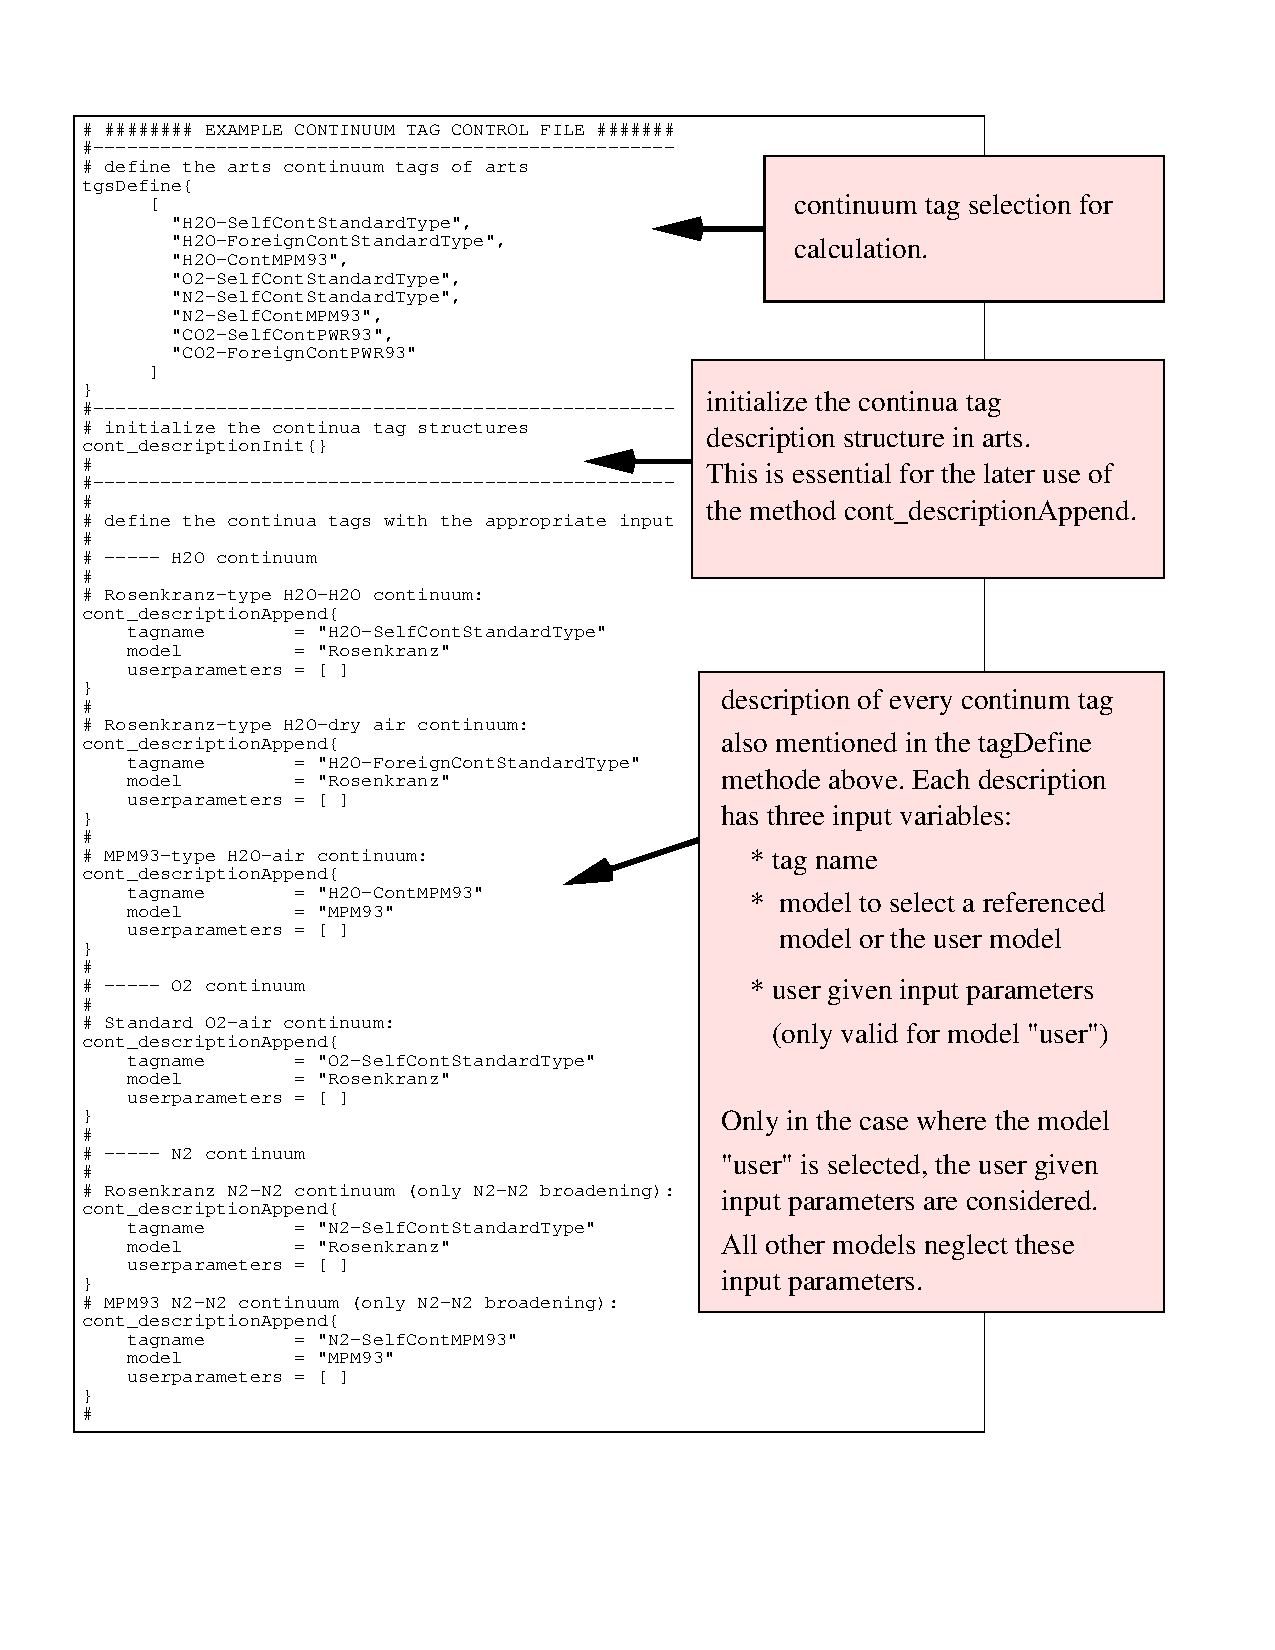
\includegraphics[scale=0.65, angle=0]{cont_description_page1}
\end{flushleft}
\begin{flushleft}
 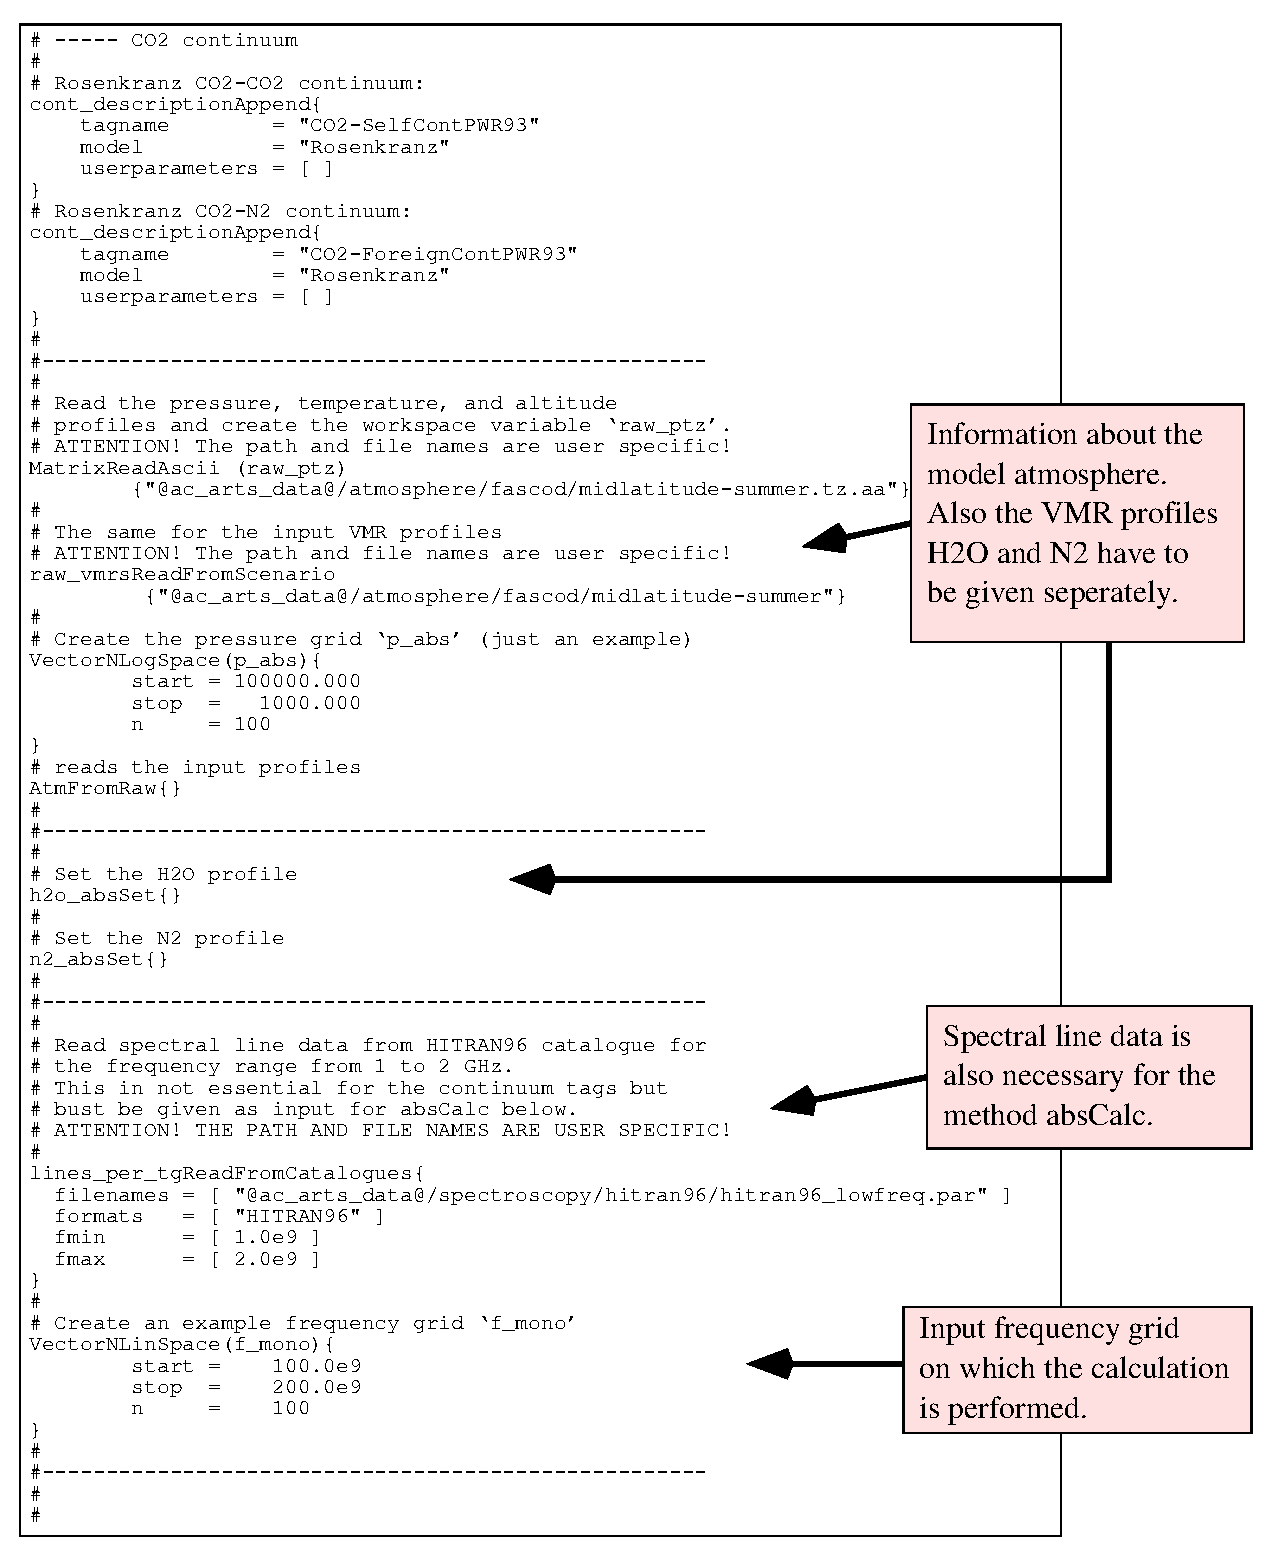
\includegraphics[scale=0.65, angle=0]{cont_description_page2}
\end{flushleft}
\begin{flushleft}
 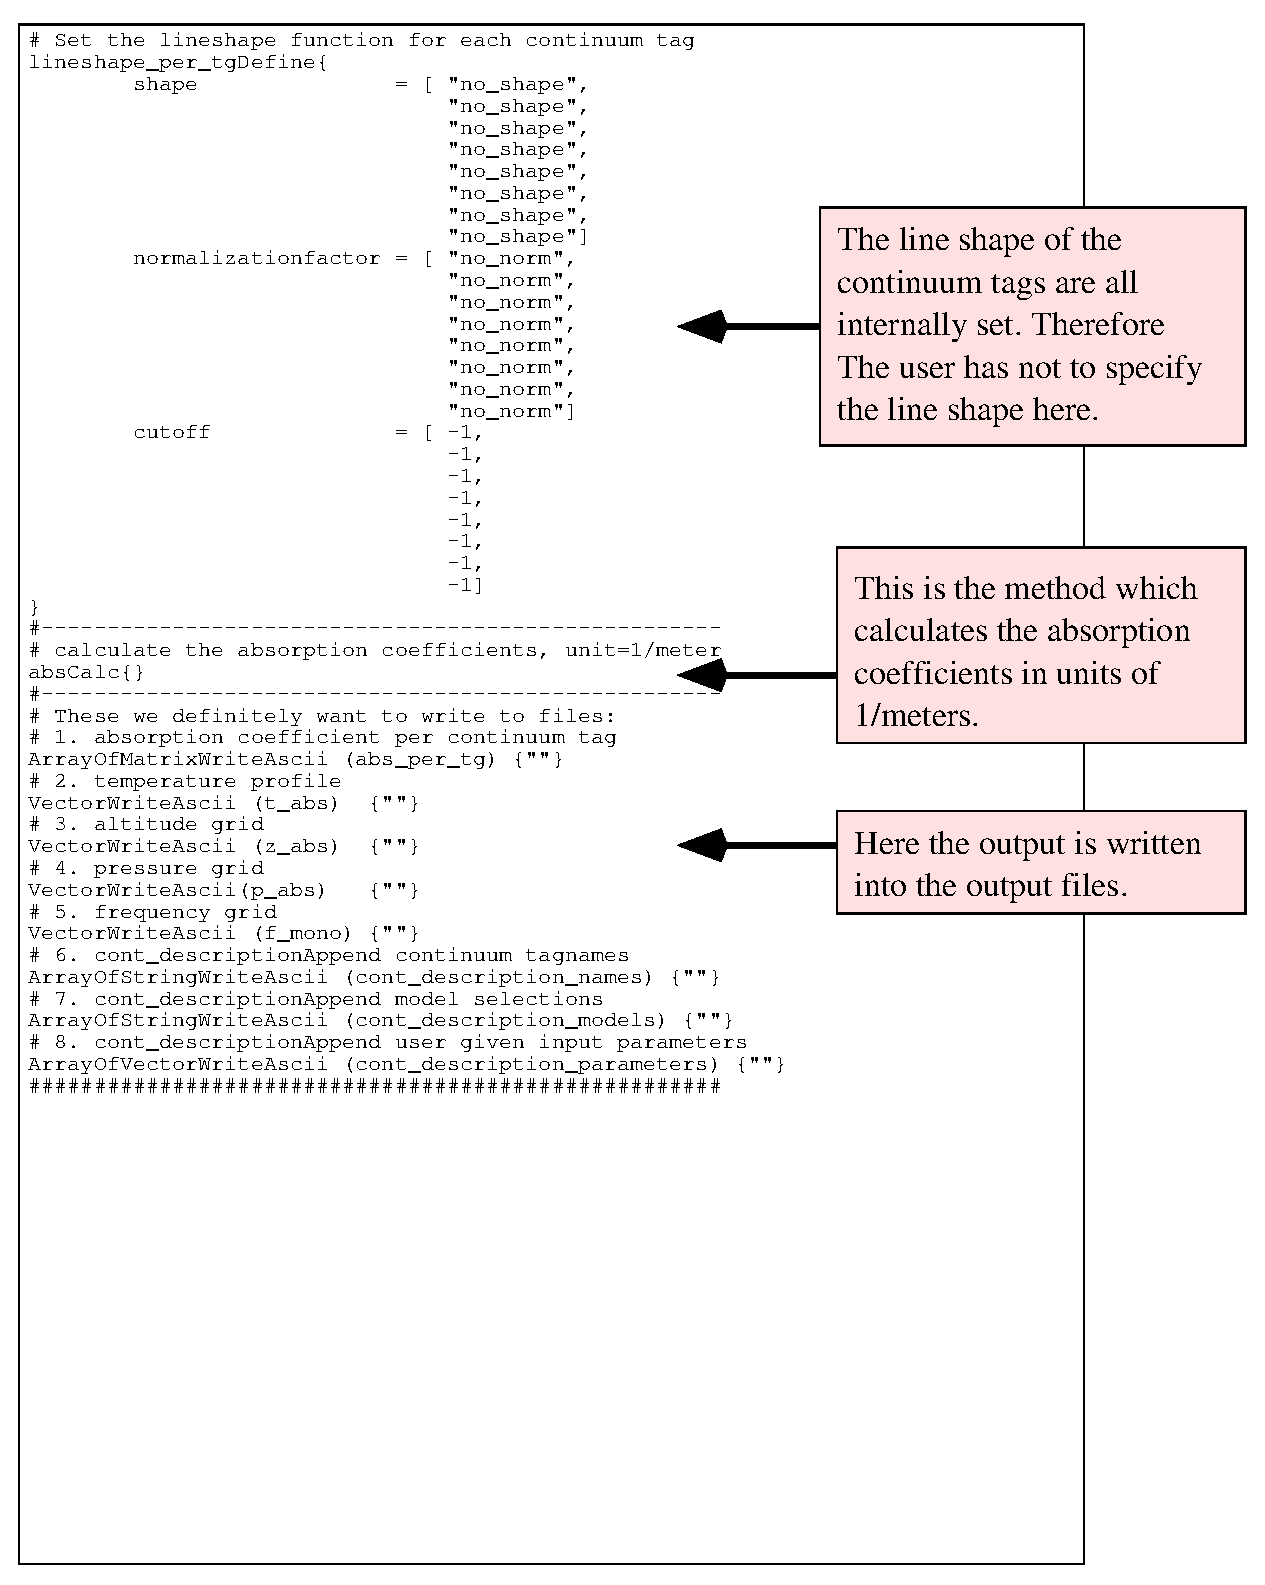
\includegraphics[scale=0.65, angle=0]{cont_description_page3}
\end{flushleft}



% ================================================================================
% The following section is written by Thomas Kuhn, iup Bremen, tkuhn@uni-bremen.de
% ================================================================================



\levelb{Complete Absorption Models}
\label{levelb:CompAbsMod}
% =================================
The MPM absorption model of Liebe and coworkers consists of modules for 
water vapor and oxygen absorption. The Rosenkranz (PWR98) absorption 
model include also $\hzo$ and $\oz$ while the Cruz-Pol et al. (CP98) absorption 
models include absorption due to water vapor. Additionally 
the CP98 model has a strongly reduced parameter set for the $\hzo$-line 
absorption since it is especially intended for the range around the 
22\,GHz water line. The MPM and R98 are valid from the microwave 
up to the submillimeter frequency range (1-1000\,GHz).

Implemented in ARTS are the following modules of the above mentioned models:
%
\begin{center}
\begin{tabular}{ll}
\hline
species & model\\
\hline
$\hzo$ & MPM87, MPM89, MPM93, PWR98, CP98 \\
$\oz$  & MPM93, PWR98 \\
\hline
\end{tabular}
\end{center}




\levelc{Complete Water Vapor Models}
\label{levelc:CompWatVapMod}
% ==================================
In ARTS several complete water vapor absorption models are implemented and 
can easily be used. Implemented models are the versions 
MPM87 \cite{liebeandlayton:87}, MPM89 \cite{liebe:89}, and 
MPM93 \cite{liebeetal:93} of the Liebe Millimeter-wave Propagation Model 
and additionally the models of Cruz-Pol et al. (CP98) \cite{cruzpol:98} 
and P.~W. Rosenkranz (PWR98) \cite{pwr:98}. 
MPM and PWR98 are especially desigend for fast absorption calculations in 
the frequency range of 1-1000\,GHz while the CP98 model is a reduced model 
for a narrow frequency band around the 22\,GHz $\hzo$-line (especially used 
by ground-based radiometers).

The total water vapor absorption ($\alphatot$) is in all the stated models 
described by a line absorption ($\alphal$) term and a continuum absorption 
($\alphac$) term: 
\begin{equation}
  \label{eq:h2o:totabs}
  \alphatot = \alphal + \alphac
\end{equation}
The main differences between the different models is the line shape used for 
$\alphal$ and the formulation of $\alphac$.

It has to be emphasized that, $\alphal$ and $\alphac$ of different
models are not necessarily compatible and should therefore not be 
interchanged between different models.


\leveld{MPM87 Water Vapor Absorption Model}
\label{leveld:mpm87}
%------------------------------------------
This version, which is described in \cite{liebeandlayton:87} and 
follows the general line of the MPM model to divide the total 
water vapor absorption, $\alphampmotot$, into a spectral line 
term, $\alphampmol$, and a continuum term not attributed to 
spectral lines, $\alphampmoc$:
\begin{equation}
  \label{eq:mpm87_abs}
  \alphampmotot = \alphampmol + \alphampmoc\hspace*{10mm}\mbox{dB/km}
\end{equation}



\levele{Water Vapor Line Absorption:}
\label{levele:mpm87_h2olines}
%-----------------------------------
The MPM87 \cite{liebeandlayton:87} water vapor line catalog consists 
of 30 lines from 22\,GHz up to 988\,GHz. The center frequencies and parameter 
values are listed in Table \ref{tab:mpm87linelist}. To describe the line 
absorption, a set of three parameters ($\bek$ and $\bdk$) per line are used: two 
for the line strength and one for the line width. The total line 
absorption coefficient (in units of dB/km) is the sum over all 
individual line absorption coefficients\footnote{The factor 
  $0.1820 \cdot 10^{6}$ is equal to $(4\,\pi/c)\cdot 10\log{(e)}$
  (the term $(4\,\pi/c)$ comes from the definition of the absorption
  coefficient in terms of the dielectric constant and the term 
  $10\,\log{(e)}$ is due to the definition of the Decibel.) The
  velocity of light is defined as $c=2.9979\cdot 10^{-4}$\,km\,GHz. 
  The factor $10^{6}$ is incorporated into the line strength and 
  does therefore not appear in the pre-factor.}:
\begin{equation}
  \label{eq:mpm87:absline}
  \alphampmol = 0.1820 \cdot \nuk \cdot \phzo \cdot 
  \sum_{k}{\inten \cdot \shape}\hspace*{10mm}\mbox{dB/km}
\end{equation}
where $\inten$ is the line intensity described by the parameterization
\begin{equation}
  \label{eq:mpm87:strength}
  \inten = \bek \cdot \phzo \cdot \Theta^{3.5} 
           \cdot \exp{(\bzk \cdot [1-\Theta])}\hspace*{10mm}\mbox{kHz}
\end{equation}
with $\nuk$ as the line center frequency, $\phzo$ the water
vapor partial pressure and $\Theta = 300\,\mbox{K}/T$.\\
The line shape function, $\shape$, in Eq.~(\ref{eq:mpm87:absline}) 
is the standard Van~Vleck-Weisskopf (VVW) function, given by:
\begin{eqnarray}
% Van Vleck-Weisskopf function
  \label{eq:mpm87:VVW}
  \shape & = & \left(\frac{\nu}{\nuk}\right) \cdot 
               \left[\frac{\gamk}{(\nu - \nuk)^2 + \gamk^2} + 
                     \frac{\gamk}{(\nu + \nuk)^2 + \gamk^2}\right]\\
\end{eqnarray}
The pressure broadened line width, $\gamk$, is calculated with the 
single parameter $\bdk$ in the following way:
\begin{equation}
  \label{eq:mpm87:gamma}
  \gamk = \bdk \cdot 
          (4.80 \cdot \phzo \cdot \Theta^{1.1} + \pda \cdot
          \Theta^{0.6})\hspace*{10mm}\mbox{GHz}
\end{equation}
where $\pda$ is the partial pressure of dry air ($\pda=\ptot-\phzo$). 
The parameterizations of $\inten$ and $\gamk$ are already in use for the 
early version of MPM81 \cite{liebe:81}.
%
\begin{longtable}{rrrrr}
 K & K & K & K & K \kill
%
% --------------------- only begin of table ------------------------------
 \hline
       & $\nu_k$ & $\bek$   & $\bzk$ & $\bdk$  \\
% //      [GHz]    [kHz/kPa]   [1]     [GHz/kPa]
 $k$   & {\rm [GHz]}  & {[$\frac{\rm kHz}{\rm kPa}$]} & {\rm [1]} & 
 {[$\frac{\rm GHz}{\rm kPa}$]}\\
 \hline
 \endfirsthead
% --------------------- every page begin of table ------------------------
 \hline
  $k$  & $\nu_k$ & $\bek$ & $\bzk$ & $\bdk$ \\
 \hline
 \endhead
% --------------------- every page end of table ------------------------
 K & K & K & K & K \kill
 \hline
 \caption[]{(continued)}\\
 \endfoot
% --------------------- only end of table ------------------------------
 K & K & K & K & K \kill 
 \hline
 \caption{List of H$_2$O spectral lines and their spectroscopic 
   parameters (H$_2$O-air mixture) for the MPM87 model \cite{liebeandlayton:87}.}
 \label{tab:mpm87linelist}
 \endlastfoot
% --------------------- body of table  ----------------------------------  
% //         0           1           2       3      
% //         f0          b1          b2      b3     
% //        [GHz]       [kHz/kPa]   [1]    [GHz/kPa]
%  const Numeric mpm87[30][4] = { 
1     &    22.235080&    0.1090&  2.143&   27.84$\cdot$ 10$^{-3}$\\
2     &    67.813960&    0.0011&  8.730&   27.60$\cdot$ 10$^{-3}$\\
3     &   119.995940&    0.0007&  8.347&   27.00$\cdot$ 10$^{-3}$\\
4     &   183.310117&    2.3000&  0.653&   31.64$\cdot$ 10$^{-3}$\\
5     &   321.225644&    0.0464&  6.156&   21.40$\cdot$ 10$^{-3}$\\
6     &   325.152919&    1.5400&  1.515&   29.70$\cdot$ 10$^{-3}$\\
7     &   336.187000&    0.0010&  9.802&   26.50$\cdot$ 10$^{-3}$\\
8     &   380.197372&   11.9000&  1.018&   30.36$\cdot$ 10$^{-3}$\\
9     &   390.134508&    0.0044&  7.318&   19.00$\cdot$ 10$^{-3}$\\
10    &   437.346667&    0.0637&  5.015&   13.70$\cdot$ 10$^{-3}$\\
11    &   439.150812&    0.9210&  3.561&   16.40$\cdot$ 10$^{-3}$\\
12    &   443.018295&    0.1940&  5.015&   14.40$\cdot$ 10$^{-3}$\\
13    &   448.001075&   10.6000&  1.370&   23.80$\cdot$ 10$^{-3}$\\
14    &   470.888947&    0.3300&  3.561&   18.20$\cdot$ 10$^{-3}$\\
15    &   474.689127&    1.2800&  2.342&   19.80$\cdot$ 10$^{-3}$\\
16    &   488.491133&    0.2530&  2.814&   24.90$\cdot$ 10$^{-3}$\\
17    &   503.568532&    0.0374&  6.693&   11.50$\cdot$ 10$^{-3}$\\
18    &   504.482692&    0.0125&  6.693&   11.90$\cdot$ 10$^{-3}$\\
19    &   556.936002&  510.0000&  0.114&   30.00$\cdot$ 10$^{-3}$\\
20    &   620.700807&    5.0900&  2.150&   22.30$\cdot$ 10$^{-3}$\\
21    &   658.006500&    0.2740&  7.767&   30.00$\cdot$ 10$^{-3}$\\
22    &   752.033227&  250.0000&  0.336&   28.60$\cdot$ 10$^{-3}$\\
23    &   841.073593&    0.0130&  8.113&   14.10$\cdot$ 10$^{-3}$\\
24    &   859.865000&    0.1330&  7.989&   28.60$\cdot$ 10$^{-3}$\\
25    &   899.407000&    0.0550&  7.845&   28.60$\cdot$ 10$^{-3}$\\
26    &   902.555000&    0.0380&  8.360&   26.40$\cdot$ 10$^{-3}$\\
27    &   906.205524&    0.1830&  5.039&   23.40$\cdot$ 10$^{-3}$\\
28    &   916.171582&    8.5600&  1.369&   25.30$\cdot$ 10$^{-3}$\\
29    &   970.315022&    9.1600&  1.842&   24.00$\cdot$ 10$^{-3}$\\
30    &   987.926764&  138.0000&  0.178&   28.60$\cdot$ 10$^{-3}$\\
\hline
% -----------------------------------------------------------------------  
\end{longtable}


\levele{Water Vapor Continuum Absorption:}
\label{levele:mpm87_h2ocont}
%----------------------------------------
The water vapor continuum absorption coefficient in MPM87, $\alphampmoc$, 
is determined from laboratory measurements at 137.8\,GHz by Liebe 
and Layton covering the following parameter range:\\
\begin{tabular}{lr}
temperature          & 282-316\,K\\
relative humidity    & 0-95\,\%\\
dry air pressure     & 0 - 160\,kPa\\ 
\end{tabular}\\
The mathematical expression of $\alphampmoc$ is derived from the far wing 
approximation of the line absorption and is expressed as follows
\begin{equation} 
  \label{eq:mpm87:cont}
  \alphampmoc = \nu^2 \cdot \phzo \cdot 
                (\cso \cdot \phzo \cdot \Theta^{\xs} + 
                 \cdo \cdot \pda  \cdot \Theta^{\xf}),
\end{equation}
with the continuum parameter set $\cso$, $\cdo$, $\xs$, and $\xf$. 
The determined values of the continuum parameters are:

\begin{description}
\item{$\cso$}   =  6.496\,$\cdot$\,10$^{-6}$~~(dB/km)~/~(hPa$\cdot$GHz)$^2$
\item{$\xs$}    = 10.5
\item{$\cdo$}   =  0.206\,$\cdot$\,10$^{-6}$~~(dB/km)~/~(hPa$\cdot$GHz)$^2$
\item{$\xd$}    =  3.0
\end{description}




\leveld{MPM89 Water Vapor Absorption Model}
\label{leveld:mpm89}
%------------------------------------------
%
MPM89 is described in \cite{liebe:89} and follows the general line 
of the MPM model to devide the total water vapor absorption, 
$\alphampmmtot$, into a spectral line term, $\alphampmml$, and a continuum 
term not attributed to spectral lines, $\alphampmmc$:
\begin{equation}
  \label{eq:mpm89_abs}
  \alphampmmtot = \alphampmml + \alphampmmc\hspace*{10mm}\mbox{dB/km}
\end{equation}
All the absorption coefficients are calculated in units of \mbox{dB/km}.


\levele{Water Vapor Line Absorption:}
\label{levele:mpm89_h2olines}
%-----------------------------------
The MPM89 water vapor line catalog consists of the same 30 lines 
like MPM87 from 22\,GHz up to 988\,GHz. The center frequencies and parameter 
values are listed in Table \ref{tab:mpm89linelist}. To describe the line 
absorption, a set of six parameters ($\bek$ and $\bsk$) per line are used: two 
for the line strength and four for the line width. The total line 
absorption coefficient (in units of dB/km) is the sum over all
individual line absorption coefficients\footnote{see footnote for
  MPM97 line absorption}:
\begin{equation}
  \label{eq:mpm89:absline}
  \alphampmml = 0.1820 \cdot \nuk \cdot \phzo \cdot 
  \sum_{k}{\inten \cdot \shape}\hspace*{10mm}\mbox{dB/km}
\end{equation}
where $\inten$ is the line intensity described by the parameterization
\begin{equation}
  \label{eq:mpm89:strength}
  \inten = \bek \cdot \phzo \cdot \Theta^{3.5} 
           \cdot \exp{(\bzk \cdot [1-\Theta])}\hspace*{10mm}\mbox{kHz}
\end{equation}
whit $\nuk$ as the line center frequency, $\phzo$ the water
vapor partial pressure and $\Theta = 300\,\mbox{K}/T$.\\
The line shape function, $\shape$, in Eq.~(\ref{eq:mpm89:absline}) 
is the standard Van Vleck-Weisskopf (VVW) function, given by 
\begin{eqnarray}
% Van Vleck-Weisskopf function
  \label{eq:mpm89:VVW}
  \shape & = & \left(\frac{\nu}{\nuk}\right) \cdot 
               \left[\frac{\gamk}{(\nu - \nuk)^2 + \gamk^2} + 
                     \frac{\gamk}{(\nu + \nuk)^2 + \gamk^2}\right]
\end{eqnarray}
where the pressure broadened line width, $\gamk$, is calculated as
\begin{equation}
  \label{eq:mpm89:gamma}
  \gamk = \bdk \cdot 
         (\bfk \cdot \phzo \cdot \Theta^{\bsk} + 
                     \pda  \cdot \Theta^{\bvk})
        \cdot 10^{-3}\hspace*{10mm}\mbox{GHz}
\end{equation}
with $\pda=\ptot-\phzo$ as the dry air partial pressure. 
The only difference between MPM87 and MPM89 with respect to the line 
absorption is the parameterization of the pressure broadened line
width, $\gamk$, which is calculated with the four parameters $\bdk$ to
$\bsk$ in the case of MPM89 whereas in MPM87 a single parameter
($\bdk$) is used (see Eq.~(\ref{eq:mpm87:gamma})).
%
\begin{longtable}{rrrrrrrr}
 K & K & K & K & K & K & K & K \kill
%
% --------------------- only begin of table ------------------------------
 \hline
    & $\nu_k$ & $\bek$ & $\bzk$ & $\bdk$ & $\bvk$ & $\bfk$ & $\bsk$ \\
%    [GHz]     [kHz/kPa]   [1]   [MHz/kPa]  [1]    [1]    [1]
 $k$& {\rm [GHz]}  & {[$\frac{\rm kHz}{\rm kPa}$]} & {\rm [1]} & 
 {[$\frac{\rm MHz}{\rm kPa}$]} & {\rm [1]} & {\rm [1]} & {\rm [1]} \\
 \hline
 \endfirsthead
% --------------------- every page begin of table ------------------------
 \hline
  $k$  & $\nu_k$ & $\bek$ & $\bzk$ & $\bdk$ & $\bvk$ & $\bfk$ & $\bsk$ \\
 \hline
 \endhead
% --------------------- every page end of table ------------------------
 K & K & K & K & K & K & K & K \kill
 \hline
 \caption[]{(continued)}\\
 \endfoot
% --------------------- only end of table ------------------------------
 K & K & K & K & K & K & K & K \kill
 \hline
 \caption{List of H$_2$O spectral lines and their spectroscopic 
   parameters (H$_2$O-air mixture) for the MPM89 model \cite{liebe:89}.}
 \label{tab:mpm89linelist}
 \endlastfoot
% --------------------- body of table  ----------------------------------  
%            0           1        2       3        4      5      6
%            f0          b1       b2      b3       b4     b5     b6
%          [GHz]     [kHz/kPa]   [1]   [MHz/kPa]  [1]    [1]    [1]
%  const Numeric mpm89[30][7] = { 
1    &    22.235080&    0.1090&  2.143&   28.11&   0.69&  4.80&  1.00\\
2    &    67.813960&    0.0011&  8.735&   28.58&   0.69&  4.93&  0.82\\
3    &   119.995940&    0.0007&  8.356&   29.48&   0.70&  4.78&  0.79\\
4    &   183.310074&    2.3000&  0.668&   28.13&   0.64&  5.30&  0.85\\
5    &   321.225644&    0.0464&  6.181&   23.03&   0.67&  4.69&  0.54\\
6    &   325.152919&    1.5400&  1.540&   27.83&   0.68&  4.85&  0.74\\
7    &   336.187000&    0.0010&  9.829&   26.93&   0.69&  4.74&  0.61\\
8    &   380.197372&   11.9000&  1.048&   28.73&   0.69&  5.38&  0.84\\
9    &   390.134508&    0.0044&  7.350&   21.52&   0.63&  4.81&  0.55\\
10    &   437.346667&    0.0637&  5.050&   18.45&   0.60&  4.23&  0.48\\
11    &   439.150812&    0.9210&  3.596&   21.00&   0.63&  4.29&  0.52\\
12    &   443.018295&    0.1940&  5.050&   18.60&   0.60&  4.23&  0.50\\
13    &   448.001075&   10.6000&  1.405&   26.32&   0.66&  4.84&  0.67\\
14    &   470.888947&    0.3300&  3.599&   21.52&   0.66&  4.57&  0.65\\
15    &   474.689127&    1.2800&  2.381&   23.55&   0.65&  4.65&  0.64\\
16    &   488.491133&    0.2530&  2.853&   26.02&   0.69&  5.04&  0.72\\
17    &   503.568532&    0.0374&  6.733&   16.12&   0.61&  3.98&  0.43\\
18    &   504.482692&    0.0125&  6.733&   16.12&   0.61&  4.01&  0.45\\
19    &   556.936002&  510.0000&  0.159&   32.10&   0.69&  4.11&  1.00\\
20    &   620.700807&    5.0900&  2.200&   24.38&   0.71&  4.68&  0.68\\
21    &   658.006500&    0.2740&  7.820&   32.10&   0.69&  4.14&  1.00\\
22    &   752.033227&  250.0000&  0.396&   30.60&   0.68&  4.09&  0.84\\
23    &   841.073593&    0.0130&  8.180&   15.90&   0.33&  5.76&  0.45\\
24    &   859.865000&    0.1330&  7.989&   30.60&   0.68&  4.09&  0.84\\
25    &   899.407000&    0.0550&  7.917&   29.85&   0.68&  4.53&  0.90\\
26    &   902.555000&    0.0380&  8.432&   28.65&   0.70&  5.10&  0.95\\
27    &   906.205524&    0.1830&  5.111&   24.08&   0.70&  4.70&  0.53\\
28    &   916.171582&    8.5600&  1.442&   26.70&   0.70&  4.78&  0.78\\
29    &   970.315022&    9.1600&  1.920&   25.50&   0.64&  4.94&  0.67\\
30    &   987.926764&  138.0000&  0.258&   29.85&   0.68&  4.55&  0.90\\
\hline
% -----------------------------------------------------------------------  
\end{longtable}


\levele{Water Vapor Continuum Absorption:}
\label{levele:mpm89_h2ocont}
%----------------------------------------
The MPM89 continuum absorption coefficients in, $\alphampmmc$, 
are identical as those in MPM87 (see Sec. \ref{levele:mpm87_h2ocont} for 
details):
\begin{equation} 
  \label{eq:mpm89:cont}
  \alphampmmc = \nu^2 \cdot \phzo \cdot 
                (\cso \cdot \phzo \cdot \Theta^{\xs} + 
                 \cdo \cdot \pda  \cdot \Theta^{\xf}),
\end{equation}
with
\begin{description}
\item{$\cso$}   =  6.496\,$\cdot$\,10$^{-6}$~~(dB/km)~/~(hPa$\cdot$GHz)$^2$
\item{$\xs$}    = 10.5
\item{$\cdo$}   =  0.206\,$\cdot$\,10$^{-6}$~~(dB/km)~/~(hPa$\cdot$GHz)$^2$
\item{$\xd$}    =  3.0
\end{description}





\leveld{MPM93 Water Vapor Absorption Model}
\label{leveld:mpm93}
%----------------------------------------------
This version, which is described in \cite{liebeetal:93} and 
follows the general line of the MPM model to devide the total 
water vapor absorption, $\alphampmntot$, into a spectral line 
term, $\alphampmnl$, and a continuum term not attributed to 
spectral lines, $\alphampmnc$:
\begin{equation}
  \label{eq:mpm93_abs}
  \alphampmntot = \alphampmnl + \alphampmnc\hspace*{10mm}\mbox{dB/km}
\end{equation}
The continuum absorption is parameterized like a
resonant spectral line of $\hzo$, a so-called pseudo-line. This is a 
fundamental change in the parameterization of the water vapor
continuum in respect to all older versions of MPM, which makes it 
quite complicate to compare the different versions, especially to 
distinguish a self- and foreign broadening term in the continuum.



\levele{Water Vapor Line Absorption:}
\label{levele:mpm93_h2olines}
%-----------------------------------
The water vapor line spectrum of MPM93 \cite{liebeetal:93} 
consists of 34 lines below 1\,THz (four more than in MPM89 and MPM87). 
To describe the MPM93 water vapor line absorption, a set of six parameters 
($\bek$ and $\bdk$) per line are used: two for the line strength and 
four for the line width. The total line absorption coefficient 
(in units of dB/km) is the sum over all individual line absorption 
coefficients\footnote{see footnote for MPM97 line absorption}:
\begin{equation}
  \label{eq:mpm93:absline}
  \alphampmnl = 0.1820 \cdot \nuk \cdot \phzo \cdot 
  \sum_{k}{\inten \cdot \shape}\hspace*{10mm}\mbox{dB/km}
\end{equation}
where $\inten$ is the line intensity described by the parameterization
\begin{equation}
  \label{eq:mpm93:strength}
  \inten = \bek \cdot \phzo \cdot \Theta^{3.5} 
           \cdot \exp{(\bzk \cdot [1-\Theta])}\hspace*{10mm}\mbox{kHz}
\end{equation}
with $\nuk$ as the line center frequency, $\phzo$ the water
vapor partial pressure and $\Theta = 300\,\mbox{K}/T$.\\
The line shape function, $\shape$, in Eq.~(\ref{eq:mpm87:absline}) 
is the standard Van~Vleck-Weisskopf (VVW) function, given by:
\begin{eqnarray}
% Van Vleck-Weisskopf function
  \label{eq:mpm93:VVW}
  \shape & = & \left(\frac{\nu}{\nuk}\right) \cdot 
               \left[\frac{\gamk}{(\nu - \nuk)^2 + \gamk^2} + 
                     \frac{\gamk}{(\nu + \nuk)^2 + \gamk^2}\right]\\
\end{eqnarray}
The pressure broadened line width, $\gamk$, is calculated with the 
single parameter $\bdk$ in the following way:
\begin{equation}
  \label{eq:mpm93:gamma}
  \gamk = \bdk \cdot 
          (4.80 \cdot \phzo \cdot \Theta^{1.1} + \pda \cdot
          \Theta^{0.6})\hspace*{10mm}\mbox{GHz}
\end{equation}
where $\pda$ is the partial pressure of dry air ($\pda=\ptot-\phzo$). 

The parameterizations of $\inten$ was already in use for the early 
version of MPM81 \cite{liebe:81}. The expression for $\gamk$ is the
same as in MPM89. The main difference between MPM93 and MPM89 
concerning the water vapor line absorption is the updated line catalog.
%
%
%\begin{landscape}
%\setlength{\LTcapwidth}{200mm} % with of the caption in longtable
\begin{longtable}{rrrrrrrr}
 K & K & K & K & K & K & K & K \kill
%
% --------------------- only begin of table ------------------------------
 \hline
       & $\nu_k$ & $\bek$ & $\bzk$ & $\bdk$ & $\bvk$ & $\bfk$ & $\bsk$ \\
 $k$   & {\rm [GHz]}  & {[$\frac{\rm kHz}{\rm hPa}$]} & {\rm [1]} & 
 {[$\frac{\rm MHz}{\rm hPa}$]} & {\rm [1]} & {\rm [1]} & {\rm [1]} \\
 \hline
 \endfirsthead
% --------------------- every page begin of table ------------------------
 \hline
    & $\nu_k$ & $\bek$ & $\bzk$ & $\bdk$ & $\bvk$ & $\bfk$ & $\bsk$ \\
 \hline
 \endhead
% --------------------- every page end of table ------------------------
 K & K & K & K & K & K & K & K \kill
 \hline
 \caption[]{(continued)}\\
 \endfoot
% --------------------- only end of table ------------------------------
 K & K & K & K & K & K & K & K \kill
 \hline
 \caption{List of used H$_2$O spectral lines and their spectroscopic 
   coefficients of H$_2$O in air for the MPM93 model \citep{liebeetal:93}. 
   The last separated line is the unphysical pseudo-line used in MPM93. 
   The lines which are marked with a "$^+$" were not in the MPM87/MPM89 
   line catalog.}
 \label{tab:mpm93linelist}
 \endlastfoot
% --------------------- body of table  ----------------------------------  
1      & 22.235080  & 0.01130 & 2.143 & 2.811 & 4.80 & 0.69 & 1.00 \\
2      & 67.803960  & 0.00012 & 8.735 & 2.858 & 4.93 & 0.69 & 0.82 \\
3      & 119.995940 & 0.00008 & 8.356 & 2.948 & 4.78 & 0.70 & 0.79 \\
4      & 183.310091 & 0.24200 & 0.668 & 3.050 & 5.30 & 0.64 & 0.85 \\
5      & 321.225644 & 0.00483 & 6.181 & 2.303 & 4.69 & 0.67 & 0.54 \\ 
6      & 325.152919 & 0.14990 & 1.540 & 2.783 & 4.85 & 0.68 & 0.74 \\
7      & 336.222601 & 0.00011 & 9.829 & 2.693 & 4.74 & 0.69 & 0.61 \\ 
8      & 380.197372 & 1.15200 & 1.048 & 2.873 & 5.38 & 0.54 & 0.89 \\
9      & 390.134508 & 0.00046 & 7.350 & 2.152 & 4.81 & 0.63 & 0.55 \\
10     & 437.346667 & 0.00650 & 5.050 & 1.845 & 4.23 & 0.60 & 0.48 \\
11     & 439.150812 & 0.09218 & 3.596 & 2.100 & 4.29 & 0.63 & 0.52 \\
12     & 443.018295 & 0.01976 & 5.050 & 1.860 & 4.23 & 0.60 & 0.50 \\
13     & 448.001075 & 1.03200 & 1.405 & 2.632 & 4.84 & 0.66 & 0.67 \\
14     & 470.888947 & 0.03297 & 3.599 & 2.152 & 4.57 & 0.66 & 0.65 \\
15     & 474.689127 & 0.12620 & 2.381 & 2.355 & 4.65 & 0.65 & 0.64 \\
16     & 488.491133 & 0.02520 & 2.853 & 2.602 & 5.04 & 0.69 & 0.72 \\
17     & 503.568532 & 0.00390 & 6.733 & 1.612 & 3.98 & 0.61 & 0.43 \\
18     & 504.482692 & 0.00130 & 6.733 & 1.612 & 4.01 & 0.61 & 0.45 \\
19$^+$ & 547.676440 & 0.97010 & 0.114 & 2.600 & 4.50 & 0.70 & 1.00 \\
20$^+$ & 552.020960 & 1.47700 & 0.114 & 2.600 & 4.50 & 0.70 & 1.00 \\
21     & 556.936002 & 48.74000& 0.159 & 3.210 & 4.11 & 0.69 & 1.00 \\
22     & 620.700807 & 0.50120 & 2.200 & 2.438 & 4.68 & 0.71 & 0.68 \\
23$^+$ & 645.866155 & 0.00713 & 8.580 & 1.800 & 4.00 & 0.60 & 0.50 \\
24     & 658.005280 & 0.03022 & 7.820 & 3.210 & 4.14 & 0.69 & 1.00 \\
25     & 752.033227 & 23.96000& 0.396 & 3.060 & 4.09 & 0.68 & 0.84 \\
26     & 841.053973 & 0.00140 & 8.180 & 1.590 & 5.76 & 0.33 & 0.45 \\
27     & 859.962313 & 0.01472 & 7.989 & 3.060 & 4.09 & 0.68 & 0.84 \\
28     & 899.306675 & 0.00605 & 7.917 & 2.985 & 4.53 & 0.68 & 0.90 \\
29     & 902.616173 & 0.00426 & 8.432 & 2.865 & 5.10 & 0.70 & 0.95 \\
30     & 906.207325 & 0.01876 & 5.111 & 2.408 & 4.70 & 0.70 & 0.53 \\
31     & 916.171582 & 0.83400 & 1.442 & 2.670 & 4.78 & 0.70 & 0.78 \\
32$^+$ & 923.118427 & 0.00869 & 10.220& 2.900 & 5.00 & 0.70 & 0.80 \\
33     & 970.315022 & 0.89720 & 1.920 & 2.550 & 4.94 & 0.64 & 0.67 \\
34     & 987.926764 & 13.21000& 0.258 & 2.985 & 4.55 & 0.68 & 0.90 \\
\hline
 & $\nu^*$ & $\beks$ & $\bzks$ & $\bdks$ & $\bvks$ & $\bfks$ & $\bsks$\\
 & {\rm [GHz]}  & {[$\frac{\rm kHz}{\rm hPa}$]} & {\rm [1]} & 
 {[$\frac{\rm MHz}{\rm hPa}$]} & {\rm [1]} & {\rm [1]} & {\rm [1]} \\
\hline
 & 1780.000000 & 2230.00000 & 0.952 & 17.620 & 30.50 & 2.00 & 5.00 \\
% -----------------------------------------------------------------------  
\end{longtable}
%\setlength{\LTcapwidth}{0.8\textwidth}
%\end{landscape}



\levele{The MPM93 Continuum Parameterization:}
\label{levele:mpm93:h2ocont}
%-----------------------------------------------
In the MPM93 version the water vapor continuum is parameterized as an
ordinary spectral line (Eqs. (\ref{eq:mpm93:strength}, 
\ref{eq:mpm93:VVW})). The parameters of this continuum "pseudo-line" 
($\nu^*$, $\beks$, $\bzks$, $\bdks$, $\bvks$, $\bfks$, $\bsks$) 
are given in Table \ref{tab:mpm93linelist}. More details about 
this continuum parameterization and its microwave approximation can be 
found in Section \ref{leveld:h2o_Cont} of this guide.




\leveld{CP98 Water Vapor Absorption Model}
\label{leveld:cp98}
%---------------------------------------------

\levele{Line Absorption}
\label{levele:cp98_h2oline}
%--------------------------
component \citep{cruzpol:98} for the water vapor line absorption 
is based on MPM87 with the main difference that the 
line catalog consists of only a single line at $\nu_{\rm o}=$\,22\,GHz. 
The contributions from the other lines is put into the water vapor 
continuum module. The line absorption is therefore very quickly 
calculated (in units of Np/km) according to the formula
\begin{eqnarray}
  \label{eq:cp98:lineabs}
  \alphacpl &=& 0.0419 \cdot \intencp \cdot \shape \\
  \mbox{with} & & \nonumber\\
  \label{eq:cp98:inten}
  \intencp    &=& 0.0109 \cdot C_L \cdot \phzo \cdot \nuo \cdot \Theta^{3.5} 
             \cdot \exp{(2.143\cdot[1-\Theta])}\nonumber\\
%
  \label{eq:cp98:width}
  \gamma &=& 0.002784 \cdot C_W \cdot (\pda \cdot \Theta^{0.6}+ 
             4.8 \cdot \phzo \cdot \Theta^{1.1}) \nonumber\\
\end{eqnarray}
where $\phzo$ and $\pda$ are the partial pressure of water vapor and dry
air in units of hPa, respectively and the Van Vleck-Weisskopf line
shape, $\shape$. The numbers correspond to the line
parameters form MPM87 for this special line and the factors  
$C_L$ and $C_W$ are adjustable scaling factors to match the model with the
measurements. Setting the scaling factors to $C_L$=1.00 and $C_W$=1.00 
leads to the same results as for MPM87. According to the parameter 
estimation of Cruz--Pol et al. best agreement between 
data and model is obtained with $C_L=$\,1.0639$\pm$0.016 and 
$C_W=$\,1.0658$\pm$0.0096. The correlation between these two scaling 
factors was found to be negligible, as can be seen from 
Table \ref{tab:cp_orr}.

\begin{table}[!htb]
\begin{center}
\begin{tabular}{lllll}
\hline
            & $C_L$ & $C_W$ & $C_C$ & $C_X$ \\
\hline
value       & 1.0639 & 1.0658 & 1.2369 & 1.0739\\
std. dev.   & 0.016  & 0.0096 & 0.155  & 0.252\\
\hline
correlation & &&&\\
$C_L$       & 1      & -0.085 & 0.045  & -0.048\\
$C_W$       & -0.085 & 1      & -0.513 &  0.485\\
$C_C$       & 0.045  & -0.513 & 1      & -0.989\\
$C_X$       & -0.048 & 0.485  & -0.989 & 1\\
\hline
\end{tabular}
\end{center}
\caption{Scaling parameter values with standard deviation and 
  correlation coefficients according to \citep{cruzpol:98}.
  The scaling parameters are $C_L$:22\,GHz line strength, 
  $C_W$:22\,GHz line width , $C_C$:$\hzo$-continuum, and 
  $C_X$:$\oz$-absorption. $C_X$ scales the entire oxygen absorption, 
  the continuum as well as the line absorption. The Cruz-Pol et al.
  model uses the \cite{pwr:93} oxygen absorption model.}
\label{tab:cp_orr}
\end{table}

The main reason why the Cruz-Pol model (CP98) considers only one line
lies in the fact that CP98 is especially designed for the data analysis
in the 20-31.4\,GHz region. The determination of the scaling factors was 
performed with ground based radiometer data in the frequency range of
from different locations\footnote{The data were recorded at San Diego, 
California (11. December 1991) and West Palm Beach, Florida 
(8.-21. March 1992)} in the USA.


\levele{Water Vapor Continuum Absorption:}
\label{levele:cp98_h2ocont}
%-----------------------------------------
The CP98 model uses the same water vapor continuum 
parameterization as MPM87, just scaled with an empirical 
factor, $CC$, determined from the above mentioned data:
\begin{equation}
 \label{eq:cp98_cont_scaling}
 \alphacpc = C_C \cdot \alphampmoc 
\end{equation}
The scaling factor $C_C$, as given in Table \ref{tab:cp_orr}, 
gives a 23.69\,\% increased continuum absorption compared 
with MPM87 (see Table \ref{tab:wvcontparam} for a comparison of the 
parameter values). But one has to keep in mind that $C_C$ has a 
high correlation with the scaling factor of the oxygen 
absorption, $C_X$, since these two components could not 
be completely distinguished in the data. Therefore the 
value of 23.69\,\% has a standard deviation of 15.5\,\% 
and is not so reliable than $C_L$ and $C_W$.





\leveld{PWR98 Water Vapor Absorption Model}
\label{leveld:pwr98_h2o}
%------------------------------------------
The water vapor continuum formulation of \citet{pwr:98} is a re-investigation 
of the existing models MPM87/MPM89, MPM93, and CKD\_2.1 especially for 
the frequency region below 1-1000\,GHz. in the context of the available
laboratory and atmospheric data \citep{abaueretal:89, abaueretal:93, 
abaueretal:95, beckerautler:46, englishetal:94, godonetal:92,
liebe:84, liebeandlayton:87, westwateretal:90}.

Rosenkranz adopted the structure of MPM89 for his improved model (R98). 
However, some important differences exist compared with MPM89:
\begin{itemize}
\item the water vapor line catalogs are different 
\item the R98 uses the Van~Vleck--Weisskopf line shape function with 
      cutoff and MPM89 without cutoff
\end{itemize}


\levele{Water Vapor Line Absorption:}
\label{levele:pwr98_h2oline}
%------------------------------------
The local line absorption is defined as 
\begin{eqnarray} 
 \label{eq:pwr98absline}
 \alphapwrl &=& N_{H_2O} \cdot \sum_k \inten \cdot \shapec \nonumber\\
            &=& N_{H_2O} \cdot \sum_k \inten \cdot 
                \left (\displaystyle{\frac{\nu}{\nuk}}\right )^2  \cdot 
                \left [\shapefp + \shapefm \right]~~\mbox{Np/km}
\end{eqnarray}
where $N_{H_2O}$ is the number density of water molecules, $\nu$ the
frequency and $S$ the line intensity, calculated from the HITRAN92
data base \citet{rothman:92}. Considered for this re-investigation are 
15 lines with a frequency lower than 1\,THz as listed in 
Table \ref{tab:pwr98linelist}.

The line shape function $\shapec$ has a cutoff frequency, $\nucut$,
and a baseline subtraction similar to the CKD model \cite{clough:89}.
The introduction of a cutoff frequency has two advantages: (1) the
cutoff avoids applying the line shape to distant frequencies where the 
line form is theoretically not well understood and (2) the cutoff also
establishes a limit to the summation in Eq.~(\ref{eq:pwr98absline}) where lines
far away from the cutoff limit do not contribute to the sum.  
The Rosenkranz formulation uses the same value for
the cutoff frequency as the CKD model:
\begin{equation} 
 \label{cutoff}
 \nucut = 750\mbox{ GHz}
\end{equation}
%
The explicit mathematical form of the line shape function is defined 
in such a way that in the limit $\nucut \rightarrow \infty$ the 
combination of Eq.~(\ref{eq:pwr98absline}) with the line shape function would 
be equivalent to a Van Vleck--Weisskopf \citep{vanvleck:45} line shape: 
\begin{equation}
 \label{eq:pwr98lineshape}
 \hspace*{-8mm}\shapefpm = 
   \left \{ \begin{array}{r@{\quad:\quad}l} 
   \displaystyle{\frac{\gamk}{\pi}} 
   \left \{ \displaystyle{\frac{1}{(\nu \mp \nuk)^2 + \gamk^2}} - 
   \displaystyle{\frac{1}{\nucut^2 + \gamk^2}} \right \}
   & |\nu \pm \nuk| < \nucut \\ 
   0 & |\nu \pm \nuk| \geq \nucut
                       \end{array} \right.
\end{equation}
$\nuk$ is the line center frequency and $\gamk$ the line
half width, which is calculated according to 
\begin{equation}
 \label{eq:pwr98gamma}
 \gamk = \ws \cdot \phzo \cdot \Theta^{\xs} + 
         \wf \cdot \pda  \cdot \Theta^{\xf}\hspace*{10mm}\mbox{GHz}
\end{equation}
with $\phzo$ and $\pda$ as the partial pressure of water vapor and of 
dry air, respectively. The line depending parameters $\ws$, $\xs$, 
$\wf$, and $\xf$ are listed in Table \ref{tab:pwr98linelist} and the 
dimensionless parameter $\Theta$ is defined as $\Theta$\,=\,300\,K/$T$.

Because of the structural similarity to MPM89, the line broadening 
parameters differ only in minor respects from the values used therein 
(only the parameters $x_{\rm s,1}$, $w_{\rm f,2}$ and $\rm w_{\rm s,2}$ 
are significantly different).
%
\begin{table}[!htb]
\begin{center}
\begin{tabular}{rrrrrr}
 \hline
 index &  $\nuk$      & $\wf$     & $\xf$ & $\ws$     & $\xs$ \\
   k   &  [GHz]       & [GHz/kPa] & [1]   & [GHz/kPa] & [1] \\ 
 \hline
   1   &   22.2351    & 0.00281   & 0.69  & 0.01349   &  0.61 \\
   2   &  183.3101    & 0.00281   & 0.64  & 0.01491   &  0.85 \\
   3   &  321.2256    & 0.00230   & 0.67  & 0.01080   &  0.54 \\
  4    &  325.1529    & 0.00278   & 0.68  & 0.01350   &  0.74 \\
  5    &  380.1974    & 0.00287   & 0.54  & 0.01541   &  0.89 \\
  6    &  439.1508    & 0.00210   & 0.63  & 0.00900   &  0.52 \\
  7    &  443.0183    & 0.00186   & 0.60  & 0.00788   &  0.50 \\
  8    &  448.0011    & 0.00263   & 0.66  & 0.01275   &  0.67 \\
  9    &  470.8890    & 0.00215   & 0.66  & 0.00983   &  0.65 \\
  10   &  474.6891    & 0.00236   & 0.65  & 0.01095   &  0.64 \\
  11   &  488.4911    & 0.00260   & 0.69  & 0.01313   &  0.72 \\
  12   &  556.9360    & 0.00321   & 0.69  & 0.01320   &  1.00 \\
  13   &  620.7008    & 0.00244   & 0.71  & 0.01140   &  0.68 \\
  14   &  752.0332    & 0.00306   & 0.68  & 0.01253   &  0.84 \\
  15   &  916.1712    & 0.00267   & 0.70  & 0.01275   &  0.78 \\
  \hline
\end{tabular}
\end{center}
  \caption{Line parameters of the Rosenkranz absorption model (R98) 
  (values taken from \citet{pwr:98}).}
\label{tab:pwr98linelist}
\end{table}



\levele{Water Vapor Continuum Absorption:}
\label{levele:pwr98_h2ocont}
%-----------------------------------------
The continuum absorption in R98 has the same functional dependence on frequency,
pressure, and temperature like in MPM87/MPM89 (see Sec. \ref{levele:mpm87_h2ocont}
for details):
\begin{equation} 
  \label{eq:pwr98:abscont}
  \alphapwrc = \nu^2 \cdot \phzo \cdot 
               (\cso \cdot \phzo \cdot \Theta^{\xs} + 
                \cdo \cdot \pda  \cdot \Theta^{\xf})
\end{equation}
with
\begin{description}
\item{$\cso$}   = 7.80\,$\cdot$\,10$^{-8}$~~(dB/km)~/~(hPa$\cdot$GHz)$^2$
\item{$\xs$}    = 7.5
\item{$\cdo$}   =  0.236\,$\cdot$\,10$^{-8}$~~(dB/km)~/~(hPa$\cdot$GHz)$^2$
\item{$\xd$}    = 3.0
\end{description}
The main difference to the MPM versions are the values of these 
parameters, since Rosenkranz used additional data to fit his set of 
parameters. A second point is the cutoff in the line shape of the line 
absorption calculation. Since this cutoff decreases the line absorption 
in the window regions, the continuum absorption tends to compensate this 
decrease to get the same total absorption as withouot cutoff. This effects 
mainly the parameters $\cso$ and $\cdo$ but has also an influence in the 
temperature dependence and therefore on $\xs$ and $\xd$.




\levelc{Complete Oxygen Models}
\label{levelc:02_models}
%==============================
%
Since the Maxwell equations are symmetric in the electric and
magnetic fields, electric as well as magnetic dipole transitions 
are both possible although magnetic dipoles are in general some
orders of magnitudes weaker and therefore not relevant in
atmospheric radiative transfer models. An exception to this is the complex 
around 60\,GHz of the paramagnetic oxygen magnetic dipole transitions. 
This bulk of lines arise due to the fact that for rotational 
quantum numbers $K>1$ the allowed transitions \mbox{$\Delta J = \pm$1} 
have an energy gap of approximately 60\,GHz.\\
The most frequently used absorption model for this absorption effect is that of
Liebe, Rosenkranz, and Hufford \cite{liebeetal:92} (also reported in 
\cite{pwr:93} with a slightly different parameterization).

For oxygen -- like for water vapor -- the total absorption 
($\alphatot$) is modelled as the line absorption ($\alphal$) plus a  
continuum absorption ($\alphac$):
\begin{equation}
  \label{eq:o2:totabs}
  \alphatot = \alphal + \alphac
\end{equation}
It has to be emphasized that, $\alphal$ and $\alphac$ of different
models are not necessarily compatible and should therefore not be interchanged.




\leveld{PWR93 Oxygen Absorption Model}
\label{leveld:O2_pwr98}
%-------------------------------------


\levele{Resonant Oxygen Absorption}
%\label{levele:02_pwr98_line}
\label{levele:pwr93_o2lines}
%----------------------------------
The oxygen absorption model of Rosenkranz is described in \cite{pwr:93}. It 
is based on the investigations made by Liebe, Rosenkranz, and Hufford 
\cite{liebeetal:92}. The FORTRAN77 computer program of Rosenkranz for 
the $\oz$ absorption calculation can be downloaded via anonymous ftp from 
mesa.mit.edu/phil/lbl\_rt.

The oxygen line catalog has 40 lines from which 33 lines build the 
complex around 60\,GHz. The parameterization of the line absorption,
$\alphapwrl$, is:
\begin{eqnarray}
% line ansorption:
  \alphapwrl & = & \frac{n_{\rm O_2}}{\pi} \cdot 
                   \sum_{k=1}^{40}{S_k(T) \cdot F(\nu,\nu_k)}\\
%
% \mbox{with} &   &\nonumber\\
%
% line intensity:
 & & \mbox{line intensity:} \nonumber\\
      \label{eq:PWR93:O2_abs_inten}
      S_k(T) & = & S_k(300\,{\rm K})~~/~~\exp{(b_k \cdot \Theta)}\\
% line shape:
 & & \mbox{line shape function:} \nonumber\\
   F(\nu,\nu_k) & = & \left(\frac{\nu}{\nuk}\right)^2 \cdot 
                   \left[\frac{\Gamma_k+(\nu-\nuk)\cdot Y_k}
                              {(\nu-\nu_k)^2+\Gamma_k^2}~~+~~
                         \frac{\Gamma_k-(\nu+\nuk)\cdot Y_k}
                              {(\nu+\nu_k)^2+\Gamma_k^2}\right] \nonumber\\
% line width:
 & & \mbox{line width:} \nonumber\\
    \label{eq:PWR93:O2_gamma}
    \Gamma_k & = & w_k \cdot \left(          \pda  \cdot \Theta^{0.8} + 
                                   1.1 \cdot \phzo \cdot \Theta \right)\\
% line coupling:
 & & \mbox{line coupling:} \nonumber\\
         \label{eq:PWR93:O2_coupling}
         Y_k & = & \pdair \cdot \Theta^{0.8} \cdot 
                   \left[ y_k + (\Theta-1) \cdot v_k \right]\nonumber\\
% O2 number density:
 & & \mbox{number density of $\oz$:} \nonumber\\
           n_{\rm O_2} & = & (0.20946 \cdot \pdair)/(k_B \cdot T)\nonumber\\
           \nonumber
\end{eqnarray}
where $S_k(300\,{\rm K})$ denotes the reference line
intensity at T=300\,K ant the exponential term approximates the exact 
partition function. All model parameters (see Refs. \cite{pwr:93} and \cite{liebeetal:92}
for the laboratory measurements and the fitting parameters) are 
tabulated in Table \ref{tab:pwr02line}.
%
%\setlength{\LTcapwidth}{200mm} % with of the caption in longtable
\begin{longtable}{lrrrrrr}
 K & K & K & K & K & K & K \kill
%
% --------------------- only begin of table ------------------------------
 \hline
 index & 
 $\nuk$ & 
 $S_k(300\,{\rm K})$ & 
 $b_k$ & 
 $w_k$  & 
 $y_k$ & 
 $v_k$ \\
 $k$   & 
 {\rm [GHz]}  & 
 {\rm [cm$^2$\,Hz]} & 
 {\rm [1]} & 
 {[$\frac{\rm MHz}{\rm hPa}$]} & 
 {[$\frac{\rm 10{^{-3}}}{\rm hPa}$]} & 
 {[$\frac{\rm 10{^{-3}}}{\rm hPa}$]} \\
 \hline
 \endfirsthead
% --------------------- every page begin of table ------------------------
 \hline
 index & 
 $\nuk$ & 
 $S_k(300\,{\rm K})$ & 
 $b_k$ & 
 $w_k$  & 
 $y_k$ & 
 $v_k$ \\
 \hline
 \endhead
% --------------------- every page end of table ------------------------
 K & K & K & K & K & K & K \kill
 \hline
 \caption[]{(continued)}\\
 \endfoot
% --------------------- only end of table ------------------------------
 K & K & K & K & K & K & K \kill
 \hline
 \caption{List of $\oz$ spectral lines of the Rosenkranz absorption 
          model \cite{pwr:93}.}
 \label{tab:pwr02line}
 \endlastfoot
% --------------------- body of table ----------------------------------  
1  & 118.7503  & .2936$\cdot$\,10$^{-14}$ & .009 & 1.63 & -0.0233 & 0.0079 \\
2  & 56.2648 & .8079$\cdot$\,10$^{-15}$ & .015 & 1.646 & 0.2408 & -0.0978 \\
3  & 62.4863 & .2480$\cdot$\,10$^{-14}$ & .083 & 1.468 & -0.3486 &  0.0844 \\
4  & 58.4466 & .2228$\cdot$\,10$^{-14}$ & .084 & 1.449 & 0.5227 & -0.1273 \\
5  & 60.3061 & .3351$\cdot$\,10$^{-14}$ & .212 & 1.382 & -0.5430 & 0.0699 \\
6  & 59.5910 & .3292$\cdot$\,10$^{-14}$ & .212 & 1.360 & 0.5877 & -0.0776 \\
7  & 59.1642 & .3721$\cdot$\,10$^{-14}$ & .391 & 1.319 & -0.3970 & 0.2309 \\
8  & 60.4348 & .3891$\cdot$\,10$^{-14}$ & .391 & 1.297 & 0.3237 & -0.2825 \\
9  & 58.3239 & .3640$\cdot$\,10$^{-14}$ & .626 & 1.266 & -0.1348 &  0.0436 \\
10 & 61.1506 & .4005$\cdot$\,10$^{-14}$ & .626 & 1.248 & 0.0311 & -0.0584 \\
11 & 57.6125 & .3227$\cdot$\,10$^{-14}$ & .915 & 1.221 & 0.0725 & 0.6056 \\
12 & 61.8002 & .3715$\cdot$\,10$^{-14}$ & .915 & 1.207 & -0.1663 & -0.6619 \\
13 & 56.9682 & .2627$\cdot$\,10$^{-14}$ & 1.260 & 1.181 & 0.2832 & 0.6451 \\
14 & 62.4112 & .3156$\cdot$\,10$^{-14}$ & 1.260 & 1.171 & -0.3629 & -0.6759 \\
15 & 56.3634 & .1982$\cdot$\,10$^{-14}$ & 1.660 & 1.144 & 0.3970 &  0.6547 \\
16 & 62.9980 & .2477$\cdot$\,10$^{-14}$ & 1.665 & 1.139 & -0.4599 & -0.6675 \\
17 & 55.7838 & .1391$\cdot$\,10$^{-14}$ & 2.119 & 1.110 & 0.4695 & 0.6135 \\
18 & 63.5685 & .1808$\cdot$\,10$^{-14}$ & 2.115 & 1.108 & -0.5199 & -0.6139 \\
19 & 55.2214 & .9124$\cdot$\,10$^{-15}$ & 2.624 & 1.079 & 0.5187 & 0.2952 \\
20 & 64.1278 & .1230$\cdot$\,10$^{-14}$ & 2.625 & 1.078 & -0.5597 & -0.2895 \\
21 & 54.6712 & .5603$\cdot$\,10$^{-15}$ & 3.194 & 1.05 & 0.5903 & 0.2654 \\
22 & 64.6789 & .7842$\cdot$\,10$^{-15}$ & 3.194 & 1.05 & -0.6246 & -0.2590 \\
23 & 54.1300 & .3228$\cdot$\,10$^{-15}$ & 3.814 & 1.02 & 0.6656 & 0.3750 \\
24 & 65.2241 & .4689$\cdot$\,10$^{-15}$ & 3.814 & 1.02 & -0.6942 & -0.3680 \\
25 & 53.5957 & .1748$\cdot$\,10$^{-15}$ & 4.484 & 1.00 & 0.7086 & 0.5085 \\
26 & 65.7648 & .2632$\cdot$\,10$^{-15}$ & 4.484 & 1.00 & -0.7325 & -0.5002 \\
27 & 53.0669 & .8898$\cdot$\,10$^{-16}$ & 5.224 & .97 & 0.7348 & 0.6206 \\
28 & 66.3021 & .1389$\cdot$\,10$^{-15}$ & 5.224 & .97 & -0.7546 & -0.6091 \\
29 & 52.5424 & .4264$\cdot$\,10$^{-16}$ & 6.004 & .94 & 0.7702 & 0.6526 \\
30 & 66.8368 & .6899$\cdot$\,10$^{-16}$ & 6.004 & .94 & -0.7864 & -0.6393 \\
31 & 52.0214 & .1924$\cdot$\,10$^{-16}$ & 6.844 & .92 & 0.8083 & 0.6640 \\
32 & 67.3696 & .3229$\cdot$\,10$^{-16}$ & 6.844 & .92 & -0.8210 & -0.6475 \\
33 & 51.5034 & .8191$\cdot$\,10$^{-17}$ & 7.744 & .89 & 0.8439 & 0.6729 \\
34 & 67.9009 & .1423$\cdot$\,10$^{-16}$ & 7.744 & .89 & -0.8529 & -0.6545 \\
35 & 368.4984 & .6460$\cdot$\,10$^{-15}$ & .048 & 1.92 & 0.0000 & 0.0000 \\
36 & 424.7631 & .7047$\cdot$\,10$^{-14}$ & .044 & 1.92 & 0.0000 & 0.0000 \\
37 & 487.2494 & .3011$\cdot$\,10$^{-14}$ & .049 & 1.92 & 0.0000 & 0.0000 \\
38 & 715.3932 & .1826$\cdot$\,10$^{-14}$ & .145 & 1.81 & 0.0000 & 0.0000 \\
39 & 773.8397 & .1152$\cdot$\,10$^{-13}$ & .141 & 1.81 & 0.0000 & 0.0000 \\
40 & 834.1453 &  .3971$\cdot$\,10$^{-14}$ & .145 & 1.81 & 0.0000 & 0.0000 \\
\end{longtable}
%\setlength{\LTcapwidth}{0.8\textwidth}

\levele{Oxygen Continuum Absorption:}
\label{levele:pwr98_o2cont}
%-----------------------------------
As pointed out by Van~Vleck \cite{vv:87}, the standard theory for
non-resonant absorption is that of Debye (see also Ref. \cite{townes:55}). 
The Debye line shape is obtained from the VVW line shape function by
the limiting case $\nuk \rightarrow 0$.
Rosenkranz \cite{pwr:93} adopt the Debye theory for his models: 
\begin{eqnarray}
  \label{eq:pwr_o2cont}
  \alphac &=&  C \cdot \pda \cdot \Theta^2 \cdot 
             \frac{\nu^2 \cdot \gamma}{\nu^2+\gamma^2}\\
%
  \label{eq:pwr_o2cont_1}
  \gamma &=&  w \cdot (\pda \cdot \Theta^{0.8} + 1.1 \cdot \phzo \cdot
  \Theta)
\end{eqnarray}
The values for the parameters are $C = 1.11\cdot 10^{-5}$ dB/km/(hPa\,GHz) and 
$w = 5.6 \cdot 10^{-4}$ GHz/hPa, respectively. This absorption
term is proportional to the collision frequency of a single oxygen molecule
and thus proportional to the dry air pressure\footnote{The absorption
  due to weakly bound complexes of $\oz$--$X$ with $X=\hzo,~\nz$ is 
  treated separately and therefore not included in this Debye
  formula.}.






\leveld{MPM93 Oxygen Absorption Model}
\label{levelb:O2_mpm93}
%-------------------------------------

\levele{Oxygen Line Absorption:}
\label{levele:mpm93_o2lines}
%-------------------------------
The oxygen line catalog has 44 lines from which 37 lines build the 
complex around 60\,GHz \citep{liebeetal:93}. The parameterization 
of the line absorption, $\alphampml$, is (in units of dB/km):
\begin{eqnarray}
% line absorption:
  \alphampml & = & 0.1820 \cdot \nu^2 \cdot  
                   \sum_{k=1}^{44}{S_k(T) \cdot F(\nu,\nu_k)}~~~~\mbox{dB/km}\\
%
 \mbox{with} &   &\nonumber\\
%
% line intensity:
 & & \mbox{line intensity:} \nonumber\\
      \label{eq:MPM93:O2_inten}
      S_k(T) & = & \frac{a_{1,k}}{\nuk} \cdot \pda \cdot \Theta^3 \cdot 
                   \exp{[a_{2,k} \cdot (1-\Theta)]}\\
% line shape:
 & & \mbox{line shape function:}  \nonumber\\
 F(\nu,\nu_k) & = & \left[\frac{\gamma_k+(\nu-\nuk)\cdot \delta_k}
                               {(\nu-\nu_k)^2+\gamma_k^2}~~+~~
                          \frac{\gamma_k-(\nu+\nuk)\cdot \delta_k}
                               {(\nu+\nu_k)^2+\gamma_k^2}\right] \nonumber\\
% line width:
 & & \mbox{line width:}  \nonumber\\
     \label{eq:MPM93:O2_gamma}
     \gamma_k & = & a_{3,k} \cdot 10^{-3} \cdot 
                 \left( \pda  \cdot \Theta^{a_{4,k}} + 
                        1.10 \cdot \phzo \cdot \Theta \right)\\
% line coupling:
& &  \mbox{line coupling:}  \nonumber\\
     \label{eq:MPM93:O2_coupling}
     \delta_k & = & \pdair \cdot \Theta^{0.8} \cdot 
                   \left[ a_{5,k} + \Theta \cdot a_{6,k} \right]\nonumber
\nonumber
\end{eqnarray}
%
where $a_{1-5,k}$ are the fitted parameters due to laboratory measurements 
\cite{liebeetal:92}. All model parameters are tabulated in 
Table \ref{tab:mpm9302line}. One has to note that in the MPM93 code is a 
threshold value for $\alphampml$ implemented:
\begin{equation}
 \label{eq:mpm93O2limit}
  \alphampml = 
   \left \{ \begin{array}{r@{\quad:\quad}l} 
    \alphampml & \alphampml > 0\\
    0          & \alphampml < 0
                       \end{array} \right.
\end{equation}
Therefore the oxygen absorption in the wings of the strong $\oz$-lines 
is remarkably higher than in the R93 model.
%\setlength{\LTcapwidth}{200mm} % with of the caption in longtable
\begin{longtable}{lrrrrrrr}
 K &  K & K & K & K & K & K & K \kill
%
% --------------------- only begin of table ------------------------------
 \hline
 index & 
 $\nuk$ & 
 $a_{1,k}$ & 
 $a_{2,k}$ & 
 $a_{3,k}$ & 
 $a_{4,k}$ & 
 $a_{5,k}$ & 
 $a_{6,k}$ \\
 $k$   & 
 {\rm [GHz]}  & 
 {\rm [$\frac{\rm kHz}{\rm hPa}$]} & 
 {\rm [1]} & 
 {[$\frac{\rm MHz}{\rm hPa}$]} & 
 {\rm [1]} & 
 {[$\frac{\rm 10{^{3}}}{\rm hPa}$]} & 
 {[$\frac{\rm 10{^{3}}}{\rm hPa}$]} \\
 \hline
 \endfirsthead
% --------------------- every page begin of table ------------------------
 \hline
 index & 
 $\nuk$ & 
 $a_{1,k}$ & 
 $a_{2,k}$ & 
 $a_{3,k}$ & 
 $a_{4,k}$ & 
 $a_{5,k}$ & 
 $a_{6,k}$ \\
 \hline
 \endhead
% --------------------- every page end of table ------------------------
 K &  K & K & K & K & K & K & K \kill
 \hline
 \caption[]{(continued)}\\
 \endfoot
% --------------------- only end of table ------------------------------
 K &  K & K & K & K & K & K & K \kill
 \hline
 \caption{List of $\oz$ spectral lines of the MPM93 absorption 
          model \cite{liebeetal:93}.}
 \label{tab:mpm9302line}
 \endlastfoot
% --------------------- body of table ----------------------------------  
%  //         f0          a1       a2      a3       a4     a5     a6
%  //        [GHz]     [kHz/hPa]   [1]   [MHz/hPa]  [1]    [10^3/hPa]
%  const Numeric mpm93[44][7] = { 
1 & 50.474238 &   0.094 &  9.694 &    0.890 & 0.0 &   0.240 &    0.790\\
2 & 50.987749 &   0.246 &  8.694 &    0.910 & 0.0 &   0.220 &    0.780\\
3 & 51.503350 &   0.608 &  7.744 &    0.940 & 0.0 &   0.197 &    0.774\\
4 & 52.021410 &   1.414 &  6.844 &    0.970 & 0.0 &   0.166 &    0.764\\
5 & 52.542394 &   3.102 &  6.004 &    0.990 & 0.0 &   0.136 &    0.751\\
6 & 53.066907 &   6.410 &  5.224 &    1.020 & 0.0 &   0.131 &    0.714\\
7 & 53.595749 &  12.470 &  4.484 &    1.050 & 0.0 &   0.230 &    0.584\\
8 & 54.130000 &  22.800 &  3.814 &    1.070 & 0.0 &   0.335 &    0.431\\
9 & 54.671159 &  39.180 &  3.194 &    1.100 & 0.0 &   0.374 &    0.305\\
10 & 55.221367 &  63.160 &  2.624 &    1.130 & 0.0 &   0.258 &    0.339\\
11 & 55.783802 &  95.350 &  2.119 &    1.170 & 0.0 &  -0.166 &    0.705\\
12 & 56.264775 &  54.890 &  0.015 &    1.730 & 0.0 &   0.390 &   -0.113\\
13 & 56.363389 & 134.400 &  1.660 &    1.200 & 0.0 &  -0.297 &    0.753\\
14 & 56.968206 & 176.300 &  1.260 &    1.240 & 0.0 &  -0.416 &    0.742\\
15 & 57.612484 & 214.100 &  0.915 &    1.280 & 0.0 &  -0.613 &    0.697\\
16 & 58.323877 & 238.600 &  0.626 &    1.330 & 0.0 &  -0.205 &    0.051\\
17 & 58.446590 & 145.700 &  0.084 &    1.520 & 0.0 &   0.748 &   -0.146\\
18 & 59.164207 & 240.400 &  0.391 &    1.390 & 0.0 &  -0.722 &    0.266\\
19 & 59.590983 & 211.200 &  0.212 &    1.430 & 0.0 &   0.765 &   -0.090\\
20 & 60.306061 & 212.400 &  0.212 &    1.450 & 0.0 &  -0.705 &    0.081\\
21 & 60.434776 & 246.100 &  0.391 &    1.360 & 0.0 &   0.697 &   -0.324\\
22 & 61.150560 & 250.400 &  0.626 &    1.310 & 0.0 &   0.104 &   -0.067\\
23 & 61.800154 & 229.800 &  0.915 &    1.270 & 0.0 &   0.570 &   -0.761\\
24 & 62.411215 & 193.300 &  1.260 &    1.230 & 0.0 &   0.360 &   -0.777\\
25 & 62.486260 & 151.700 &  0.083 &    1.540 & 0.0 &  -0.498 &    0.097\\
26 & 62.997977 & 150.300 &  1.665 &    1.200 & 0.0 &   0.239 &   -0.768\\
27 & 63.568518 & 108.700 &  2.115 &    1.170 & 0.0 &   0.108 &   -0.706\\
28 & 64.127767 &  73.350 &  2.620 &    1.130 & 0.0 &  -0.311 &   -0.332\\
29 & 64.678903 &  46.350 &  3.195 &    1.100 & 0.0 &  -0.421 &   -0.298\\
30 & 65.224071 &  27.480 &  3.815 &    1.070 & 0.0 &  -0.375 &   -0.423\\
31 & 65.764772 &  15.300 &  4.485 &    1.050 & 0.0 &  -0.267 &   -0.575\\
32 & 66.302091 &   8.009 &  5.225 &    1.020 & 0.0 &  -0.168 &   -0.700\\
33 & 66.836830 &   3.946 &  6.005 &    0.990 & 0.0 &  -0.169 &   -0.735\\
34 & 67.369598 &   1.832 &  6.845 &    0.970 & 0.0 &  -0.200 &   -0.744\\
35 & 67.900867 &   0.801 &  7.745 &    0.940 & 0.0 &  -0.228 &   -0.753\\
36 & 68.431005 &   0.330 &  8.695 &    0.920 & 0.0 &  -0.240 &   -0.760\\
37 & 68.960311 &   0.128 &  9.695 &    0.900 & 0.0 &  -0.250 &   -0.765\\
38 & 118.750343 &  94.500 &  0.009 &   1.630 & 0.0 &  -0.036 &    0.009\\
39 & 368.498350 &   6.790 &  0.049 &   1.920 & 0.6 &   0.000 &    0.000\\
40 & 424.763124 &  63.800 &  0.044 &   1.930 & 0.6 &   0.000 &    0.000\\
41 & 487.249370 &  23.500 &  0.049 &   1.920 & 0.6 &   0.000 &    0.000\\
42 & 715.393150 &   9.960 &  0.145 &   1.810 & 0.6 &   0.000 &    0.000\\
43 & 773.839675 &  67.100 &  0.130 &   1.820 & 0.6 &   0.000 &    0.000\\
44 & 834.145330 &  18.000 &  0.147 &   1.810 & 0.6 &   0.000 &    0.000\\
\end{longtable}
%\setlength{\LTcapwidth}{0.8\textwidth}

\levele{Oxygen Continuum Absorption:}
\label{levele:mpm93_o2cont}
%-----------------------------------
As pointed out by Van~Vleck \cite{vv:87}, the standard theory for
non-resonant absorption is that of Debye (see also Ref. \cite{townes:55}). 
The Debye line shape is obtained from the VVW line shape function 
by the limiting case $\nuk \rightarrow 0$.
\cite{liebeetal:93} adopt the Debye theory for his model:
\begin{eqnarray}
  \label{eq:mpm93_o2cont}
  \alphac &=&  C \cdot \pda \cdot \Theta^2 \cdot 
               \frac{\nu^2 \cdot \gamma}{\nu^2+\gamma^2}\\
%
  \label{eq:mpm93_o2cont_1}
  \gamma  &=&  w \cdot \ptot \cdot \Theta^{0.8}\nonumber\\
\nonumber
\end{eqnarray}
The values for the parameters are $C = 1.11\cdot 10^{-5}$ dB/km/(hPa\,GHz) and 
$w = 5.6 \cdot 10^{-4}$ GHz/hPa, respectively. This absorption
term is proportional to the collision frequency of a single oxygen molecule
and thus proportional to the dry air pressure\footnote{The absorption
  due to weakly bound complexes of $\oz$--$X$ with $X=\hzo,~\nz$ is 
  treated separately and therefore not included in this Debye
  formula.}.




\levelc{ARTS Workspace Variables and Methods}
\label{levelc:ArtsImplementationCompleteModels}
% ---------------------------------------------

This section explains how the above described full models (continuum+lines) 
are represented in the structure of the arts source code and how 
one can invoke them in the arts control file.

The full model tags need more input specification than normal trace gas
tags. Why this is so can be seen from Eq. \ref{eq:abs_cont} and 
Table \ref{tab:wvcontparam}. For a single function for the water vapor 
continuum we find several different function parameters in the literature. 
To solve this ambiguity arts has two methods implemented which helps 
the user to select a single set of parameters in an easy way. 
In connection with this input parameters we distinguish generally two 
types, the referenced models which are taken from the literature 
(e. g. \cite{liebeetal:93} or \cite{pwr:93}) and the user model, 
for which the arts user is providing the necessary parameter values.

After selecting the continuum tag with the {\tt tagDefine} method, 
the arts user has to setup the arts internal structure (i. e. the workspace 
variables {\it cont\_description\_names, cont\_description\_models, 
and cont\_description\_parameters}) for the selected continuum tags, 
which can simply be done by putting the following line into the arts control file:
\begin{verbatim}
cont_descriptionInit{}
\end{verbatim}

After this initialization, the continuum tag specific
information has to be transfered to arts. This is possible with the 
arts method {\it cont\_descriptionAppend}, which has itself 
three input variables: {\it tagname}, {\it model}, and 
{\it userparameters}. The user has to specify these input 
variables in the arts control file for each selected continuum tag. 
Below is a list of all the implemented continuum tags and the associated
valid range of the input variables for {\it cont\_descriptionAppend}. 
For a condensed overview of the possible continuum tags and their 
referenced models see Table \ref{tab:artsfullmodlist} and the 
online documentation can be found under 
{\it arts/doc/doxygen/html/continua\_cc.html}.

One has to note at this place that the two input variables {\it model} and
{\it userparameters} are to some extend redundant. Therefore one can also 
produce an ambiguity by giving contradicting values for these two input variables.
To avoid such ambiguities the arts user should keep in mind the general 
rule that only the user model ({\it model ="user"}) needs input parameters 
via the input variable {\it userparameters}. All the referenced models 
need no input via {\it userparameters}. If you try to run the arts control 
file with a referenced model and input parameters you will get an error message.
Below in the detailed description of {\it cont\_descriptionAppend} you 
can find correct examples for all the continuum tags.

\begin{itemize}
\item[$\bullet$] The water vapor model of MPM87 \citep{liebeandlayton:87} 
     has the arts tag name {\tt "H2O-MPM87"}. The details about this water 
     vapor absorption model are described in Section \ref{leveld:mpm87}. 
     The standard way to use the full (=continuum+lines) MPM87 water 
     vapor absorption model is to set the input variable {\it model} 
     to "MPM87" and leaving the input parameter {\it userparameters} empty. 
     It might be necessary in some cases to use only the line or the 
     continuum absorption part of MPM87. This can be easily done 
     by setting {\it model} to "MPM87Lines" or "MPM87Continuum", 
     respectively (leaving the input parameter {\it userparameters} 
     empty too).\\ To have a minimum possibility of variation for MPM87, 
     arts allows to run MPM87 also with {\it model}\,=\,"user". 
     In this case the user has to provide three scaling factors,  
     $CC$, $CL$, and $CW$, with the input variable {\it userparameters}, 
     {\it userparameters}\,=\,$[$$CC$, $CL$, $CW$$]$. 
     Each line intensity $\inten$ (see Eq. (\ref{eq:mpm87:strength})) 
     is multiplied with the scaling factor $CL$, while $CW$ scales 
     each line width, $\gamk$, (see Eq. (\ref{eq:mpm87:gamma})). 
     The continuum absorption, $\alphampmoc$, 
     (see Eq. (\ref{eq:mpm87:cont})) also scales with $CC$.\\
     In the following all the valid possibilities for the
     tag {\tt "H2O-MPM87"} are listed (the values for the 
     model user are just example values): 
\begin{verbatim}
cont_descriptionAppend{
    name           = "H2O-MPM87"
    model          = "MPM87"
    userparameters = [ ]
}
cont_descriptionAppend{
    name           = "H2O-MPM87"
    model          = "MPM87Lines"
    userparameters = [ ]
}
cont_descriptionAppend{
    name           = "H2O-MPM87"
    model          = "MPM87Continuum"
    userparameters = [ ]
}
cont_descriptionAppend{
    name           = "H2O-MPM87"
    model          = "user"
    userparameters = [ 1.0, 1.0, 1.0 ]
}
\end{verbatim}

\item[$\bullet$] The full water vapor absorption model MPM89 \cite{liebe:89} 
     has the arts tag name {\tt "H2O-MPM89"}. The details about 
     this water vapor absorption model are described in 
     Section \ref{leveld:mpm89}.
     The standard way to use the full (=continuum+lines) MPM87 water 
     vapor absorption model is to set the input variable {\it model} 
     to "MPM89" and leaving the input parameter {\it userparameters} empty. 
     It might be necessary in some cases to use only the line or the 
     continuum absorption part of MPM89. This can be easily done 
     by setting {\it model} to "MPM89Lines" or "MPM89Continuum", 
     respectively (leaving the input parameter {\it userparameters} 
     empty too).\\ To have a minimum possibility of variation for MPM89, 
     arts allows to run MPM89 also with {\it model}\,=\,"user". 
     In this case the user has to provide three scaling factors,  
     $CC$, $CL$, and $CW$, with the input variable {\it userparameters}, 
     {\it userparameters}\,=\,$[$$CC$, $CL$, $CW$$]$. 
     Each line intensity $\inten$ (see Eq. (\ref{eq:mpm89:strength})) 
     is multiplied with the scaling factor $CL$, while $CW$ scales 
     each line width, $\gamk$, (see Eq. (\ref{eq:mpm89:gamma})). 
     The continuum absorption, $\alphampmmc$, 
     (see Eq. (\ref{eq:mpm89:cont})) also scales with $CC$.\\
     In the following all the valid possibilities for the
     tag {\tt "H2O-MPM89"} are listed (the values for the 
     model user are just example values): 
\begin{verbatim}
cont_descriptionAppend{
    name           = "H2O-MPM89"
    model          = "MPM89"
    userparameters = [ ]
}
cont_descriptionAppend{
    name           = "H2O-MPM89"
    model          = "MPM89Lines"
    userparameters = [ ]
}
cont_descriptionAppend{
    name           = "H2O-MPM89"
    model          = "MPM89Continuum"
    userparameters = [ ]
}
cont_descriptionAppend{
    name           = "H2O-MPM89"
    model          = "user"
    userparameters = [ 1.0, 1.0, 1.0 ]
}
\end{verbatim}
\item[$\bullet$] The water vapor model of MPM93 \cite{liebeetal:93}
     has the arts tag name {\tt H2O-MPM93}. The details about this water vapor 
     absorption model are described in Section \ref{leveld:mpm93}.
     The standard way to use the full (=continuum+lines) MPM93 water 
     vapor absorption model is to set the input variable {\it model} 
     to "MPM93" and leaving the input parameter {\it userparameters} empty. 
     It might be necessary in some cases to use only the line or the 
     continuum absorption part of MPM93. This can be easily done 
     by setting {\it model} to "MPM93Lines" or "MPM93Continuum", 
     respectively (leaving the input parameter {\it userparameters} 
     empty too).\\ To have a minimum possibility of variation for MPM93, 
     arts allows to run MPM93 also with {\it model}\,=\,"user". 
     In this case the user has to provide three scaling factors,  
     $CC$, $CL$, and $CW$, with the input variable {\it userparameters}, 
     {\it userparameters}\,=\,$[$$CC$, $CL$, $CW$$]$. 
     Each line intensity $\inten$ (see Eq. (\ref{eq:mpm93:strength})) 
     is multiplied with the scaling factor $CL$, while $CW$ scales 
     each line width, $\gamk$, (see Eq. (\ref{eq:mpm93:gamma})). 
     The continuum absorption, $\alphampmnc$, 
     (see Eq. (\ref{eq:mpm93:strength})) also scales with $CC$.\\
     In the following all the valid possibilities for the
     tag {\tt "H2O-MPM93"} are listed (the values for the 
     model user are just example values): 
\begin{verbatim}
cont_descriptionAppend{
    name           = "H2O-MPM93"
    model          = "MPM93"
    userparameters = [ ]
}
cont_descriptionAppend{
    name           = "H2O-MPM93"
    model          = "MPM93Lines"
    userparameters = [ ]
}
cont_descriptionAppend{
    name           = "H2O-MPM93"
    model          = "MPM93Continuum"
    userparameters = [ ]
}
cont_descriptionAppend{
    name           = "H2O-MPM93"
    model          = "user"
    userparameters = [ 1.0, 1.0, 1.0 ]
}
\end{verbatim}

\item[$\bullet$] The water vapor model of CP98 \citep{cruzpol:98}
     has the arts tag name {\tt "H2O-CP98"}. The details about this water 
     vapor absorption model are described in Section \ref{leveld:cp98}. 
     The standard way to use the full (=continuum+lines) CP98 water 
     vapor absorption model is to set the input variable {\it model} 
     to "CP98" and leaving the input parameter {\it userparameters} empty. 
     It might be necessary in some cases to use only the line or the 
     continuum absorption part of CP98. This can be easily done 
     by setting {\it model} to "CruzPolLines" or "CruzPolContinuum", 
     respectively (leaving the input parameter {\it userparameters} 
     empty too).\\ To have a minimum possibility of variation for CP98, 
     arts allows to run CP98 also with {\it model}\,=\,"user". 
     In this case the user has to provide three scaling factors,  
     $CC$, $CL$, and $CW$, with the input variable {\it userparameters}, 
     {\it userparameters}\,=\,$[$$CC$, $CL$, $CW$$]$. 
     Each line intensity $\inten$ (see Eq. (\ref{eq:cp98:inten})) 
     is multiplied with the scaling factor $CL$, while $CW$ scales 
     each line width, $\gamk$, (see Eq. (\ref{eq:cp98:width})). 
     The continuum absorption, $\alphacpc$, 
     (see Eq. (\ref{eq:cp98_cont_scaling})) also scales with $CC$.\\
     In the following all the valid possibilities for the
     tag {\tt "H2O-CP98"} are listed (the values for the 
     model user are just example values): 
\begin{verbatim}
cont_descriptionAppend{
    name           = "H2O-CP98"
    model          = "CruzPol"
    userparameters = [ ]
}
cont_descriptionAppend{
    name           = "H2O-CP98"
    model          = "CruzPolLines"
    userparameters = [ ]
}
cont_descriptionAppend{
    name           = "H2O-CP98"
    model          = "CruzPolContinuum"
    userparameters = [ ]
}
cont_descriptionAppend{
    name           = "H2O-CP98"
    model          = "user"
    userparameters = [ 1.0, 1.0, 1.0 ]
}
\end{verbatim}

\item[$\bullet$] The water vapor model of PWR98 \citep{pwr:98}
     has the arts tag name {\tt "H2O-PWR98"}. The details about this water 
     vapor absorption model are described in Section \ref{leveld:pwr98_h2o}. 
     The standard way to use the full (=continuum+lines) CP98 water 
     vapor absorption model is to set the input variable {\it model} 
     to "Rosenkranz" and leaving the input parameter {\it userparameters} empty. 
     It might be necessary in some cases to use only the line or the 
     continuum absorption part of PWR98. This can be easily done 
     by setting {\it model} to "RosenkranzLines" or "RosenkranzContinuum", 
     respectively (leaving the input parameter {\it userparameters} 
     empty too).\\ To have a minimum possibility of variation for CP98, 
     arts allows to run PWR98 also with {\it model}\,=\,"user". 
     In this case the user has to provide three scaling factors,  
     $CC$, $CL$, and $CW$, with the input variable {\it userparameters}, 
     {\it userparameters}\,=\,$[$$CC$, $CL$, $CW$$]$. 
     Each line intensity $\inten$ (see Eq. (\ref{eq:pwr98absline})) 
     is multiplied with the scaling factor $CL$, while $CW$ scales 
     each line width, $\gamk$, (see Eq. (\ref{eq:pwr98gamma})). 
     The continuum absorption, $\alphapwrc$, 
     (see Eq. (\ref{eq:pwr98:abscont})) also scales with $CC$.\\
     In the following all the valid possibilities for the
     tag {\tt "H2O-PWR98"} are listed (the values for the 
     model user are just example values):
\begin{verbatim}
cont_descriptionAppend{
    name           = "H2O-PWR98"
    model          = "Rosenkranz"
    userparameters = [ ]
}
cont_descriptionAppend{
    name           = "H2O-PWR98"
    model          = "RosenkranzLines"
    userparameters = [ ]
}
cont_descriptionAppend{
    name           = "H2O-PWR98"
    model          = "RosenkranzContinuum"
    userparameters = [ ]
}
cont_descriptionAppend{
    name           = "H2O-PWR98"
    model          = "user"
    userparameters = [ 1.0, 1.0, 1.0 ]
}
\end{verbatim}

\item[$\bullet$] The MPM93 full absorption model for oxygen \citep{liebeetal:93}
     has the arts tag name {\tt "O2-MPM93"}. The details about this 
     oxygen absorption model are described in Section \ref{levelb:O2_mpm93}. 
     The standard way to use the full (=continuum+lines) MPM93 oxygen 
     absorption model is to set the input variable {\it model} 
     to "MPM93" and leaving the input parameter {\it userparameters} empty. 
     It might be necessary in some cases to use only the line or the 
     continuum absorption part of MPM93. This can be easily done 
     by setting {\it model} to "MPM93Lines" or "MPM93Continuum", 
     respectively (leaving the input parameter {\it userparameters} 
     empty too).\\ To have a minimum possibility of variation for MPM93, 
     arts allows to run MPM93 also with {\it model}\,=\,"user". 
     In this case the user has to provide four scaling factors,  
     $CC$, $CL$, $CW$, and $CO$, with the input variable {\it userparameters}, 
     e. g. {\it userparameters}\,=\,$[$$CC$, $CL$, $CW$, $CO$$]$. 
     Each line intensity $\inten$ (see Eq. (\ref{eq:MPM93:O2_inten})) 
     is multiplied with the scaling factor $CL$, while $CW$ scales 
     each line width, $\gamk$, (see Eq. (\ref{eq:MPM93:O2_gamma})) and 
     $CO$ the line coupling parameter (see Eq. (\ref{eq:MPM93:O2_coupling})). 
     The continuum absorption, (see Eq. (\ref{eq:mpm93_o2cont})) 
     also scales with $CC$.\\
     In the following all the valid possibilities for the
     tag {\tt "O2-MPM93"} are listed (the values for the 
     model user are just example values):
\begin{verbatim}
cont_descriptionAppend{
    name           = "O2-MPM93"
    model          = "MPM93"
    userparameters = [ ]
}
cont_descriptionAppend{
    name           = "O2-MPM93"
    model          = "MPM93Lines"
    userparameters = [ ]
}
cont_descriptionAppend{
    name           = "O2-MPM93"
    model          = "MPM93Continuum"
    userparameters = [ ]
}
cont_descriptionAppend{
    name           = "O2-MPM93"
    model          = "user"
    userparameters = [ 1.0, 1.0, 1.0, 1.0 ]
}
\end{verbatim}

\item[$\bullet$] The PWR93 full absorption model for oxygen \citep{pwr:93}
     has the arts tag name {\tt "O2-PWR93"}. The details about this 
     oxygen absorption model are described in Section \ref{levele:pwr93_o2lines}. 
     The standard way to use the full (=continuum+lines) PWR93 oxygen 
     absorption model is to set the input variable {\it model} 
     to "Rosenkranz" and leaving the input parameter {\it userparameters} empty. 
     It might be necessary in some cases to use only the line or the 
     continuum absorption part of PWR93. This can be easily done 
     by setting {\it model} to "RosenkranzLines" or "RosenkranzContinuum", 
     respectively (leaving the input parameter {\it userparameters} 
     empty too).\\ To have a minimum possibility of variation for PWR93, 
     arts allows to run PWR93 also with {\it model}\,=\,"user". 
     In this case the user has to provide four scaling factors,  
     $CC$, $CL$, $CW$, and $CO$, with the input variable {\it userparameters}, 
     e. g. {\it userparameters}\,=\,$[$$CC$, $CL$, $CW$, $CO$$]$. 
     Each line intensity $\inten$ (see Eq. (\ref{eq:PWR93:O2_abs_inten})) 
     is multiplied with the scaling factor $CL$, while $CW$ scales 
     each line width, $\gamk$, (see Eq. (\ref{eq:PWR93:O2_gamma})) and 
     $CO$ the line coupling parameter (see Eq. \ref{eq:PWR93:O2_coupling})). 
     The continuum absorption, (see Eq. (\ref{eq:pwr_o2cont})) 
     also scales with $CC$.\\
     In the following all the valid possibilities for the
     tag {\tt "O2-PWR93"} are listed (the values for the 
     model user are just example values):
\begin{verbatim}
cont_descriptionAppend{
    name           = "O2-PWR93"
    model          = "Rosenkranz"
    userparameters = [ ]
}
cont_descriptionAppend{
    name           = "O2-PWR93"
    model          = "RosenkranzLines"
    userparameters = [ ]
}
cont_descriptionAppend{
    name           = "O2-PWR93"
    model          = "RosenkranzContinuum"
    userparameters = [ ]
}
cont_descriptionAppend{
    name           = "O2-PWR93"
    model          = "user"
    userparameters = [ 1.0, 1.0, 1.0, 1.0]
}
\end{verbatim}
\end{itemize}

\begin{landscape}
 \setlength{\LTcapwidth}{180mm} % with of the caption in longtable
 \begin{longtable}{llllll}
 K & K & K & K & K & K \kill
%
% --------------------- only begin of table ------------------------------
 \hline
 continuum & \multicolumn{3}{c}{{\it cont\_descriptionAppend} input} & 
 reference/ & arts source code function\\
 & \multicolumn{3}{c}{input parameter} & arts uguide & \\
 \hline
 \endfirsthead
% --------------------- every page begin of table ------------------------
 \hline
 continuum & \multicolumn{3}{c}{{\it cont\_descriptionAppend}} & 
 reference/ & arts source code function\\
 & \multicolumn{3}{c}{input parameter} & arts uguide & \\
 \hline
 \endhead
% --------------------- every page end of table ------------------------
 K & K & K & K & K & K \kill
 \hline
 \caption[]{(continued)}\\
 \endfoot
% --------------------- only end of table ------------------------------
 K & K & K & K & K & K \kill 
 \hline
 \caption{This table gives an overview of the implemented referenced 
   full (continua+line) absorption models and how they are specified 
   in the arts method {\it cont\_descriptionAppend}. Additionally the 
   reference and the arts source code function names (see file 
   {\it arts/src/continua.cc} are provided. The detailed online 
   documentation can be found under {\it arts/doc/doxygen/html/continua\_cc.html}).}
 \label{tab:artsfullmodlist}
 \endlastfoot
% --------------------- body of table  ----------------------------------  
 \multicolumn{6}{c}{{\bf water vapor ($\hzo$)}}\\
 \hline
 Rosenkranz  & tagname &=& {\tt "H2O-PWR98"}   & \cite{pwr:98} & PWR98H2OAbsModel\\
             & model &=& "Rosenkranz" &   &  \\ 
             & userparameters &=& [ ] &   & \\
% --------------------------------------------------------------
 Cruz-Pol    & tagname &=& {\tt "H2O-CP98"}    & \cite{cruzpol:98} & CP98H2OAbsModel\\
             & model &=& "CruzPol" &   &  \\ 
             & userparameters &=& [ ] &   & \\
% --------------------------------------------------------------
 MPM97       & tagname &=& {\tt "H2O-MPM87"}   & \cite{liebeandlayton:87} & MPM87H2OAbsModel\\
             & model &=& "MPM93" &   &  \\ 
             & userparameters &=& [ ] &   & \\
% --------------------------------------------------------------
 MPM89       & tagname &=& {\tt "H2O-MPM89"}   & \cite{liebe:89} & MPM89H2OAbsModel\\
             & model &=& "MPM93" &   &  \\ 
             & userparameters &=& [ ] &   & \\
% --------------------------------------------------------------
 MPM93       & tagname &=& {\tt "H2O-MPM93"}   & \cite{liebeetal:93} & MPM93H2OAbsModel\\
             & model &=& "MPM93" &   &  \\ 
             & userparameters &=& [ ] &   & \\
% --------------------------------------------------------------
 \hline
 \multicolumn{6}{c}{{\bf oxygen ($\oz$)}}\\
 \hline
 Rosenkranz  & tagname &=& {\tt "O2-SelfContPWR93"} & \cite{pwr:93} & PWR93O2AbsModel\\
             & model &=& "Rosenkranz" &   &  \\ 
             & userparameters &=& [ ] &   & \\
% --------------------------------------------------------------
 MPM93       & tagname &=& {\tt "O2-SelfContMPM93"} & \cite{liebeetal:93} & MPM93O2AbsModel\\
             & model &=& "MPM93" &   &  \\ 
             & userparameters &=& [ ] &   & \\
 \hline
% -----------------------------------------------------------------------  
 \end{longtable}
 \setlength{\LTcapwidth}{0.8\textwidth}
\end{landscape}






\leveld{ARTS Example Control File for the Full Model Tags}
\label{leveld:ArtsFullModelExampleControlFile}
% --------------------------------------------------------
Below you will find an example of a control file for all 
the implemented fixed full models to calculate line+continuum
absorption of water vapor and oxygen. Please note that to 
run this example control file you have to specify user 
specific paths and input file names to run it properly. 
You can find this example in the arts directory 
{\it arts/doc/examples/fullmodels\_example.arts}


\begin{flushleft}
 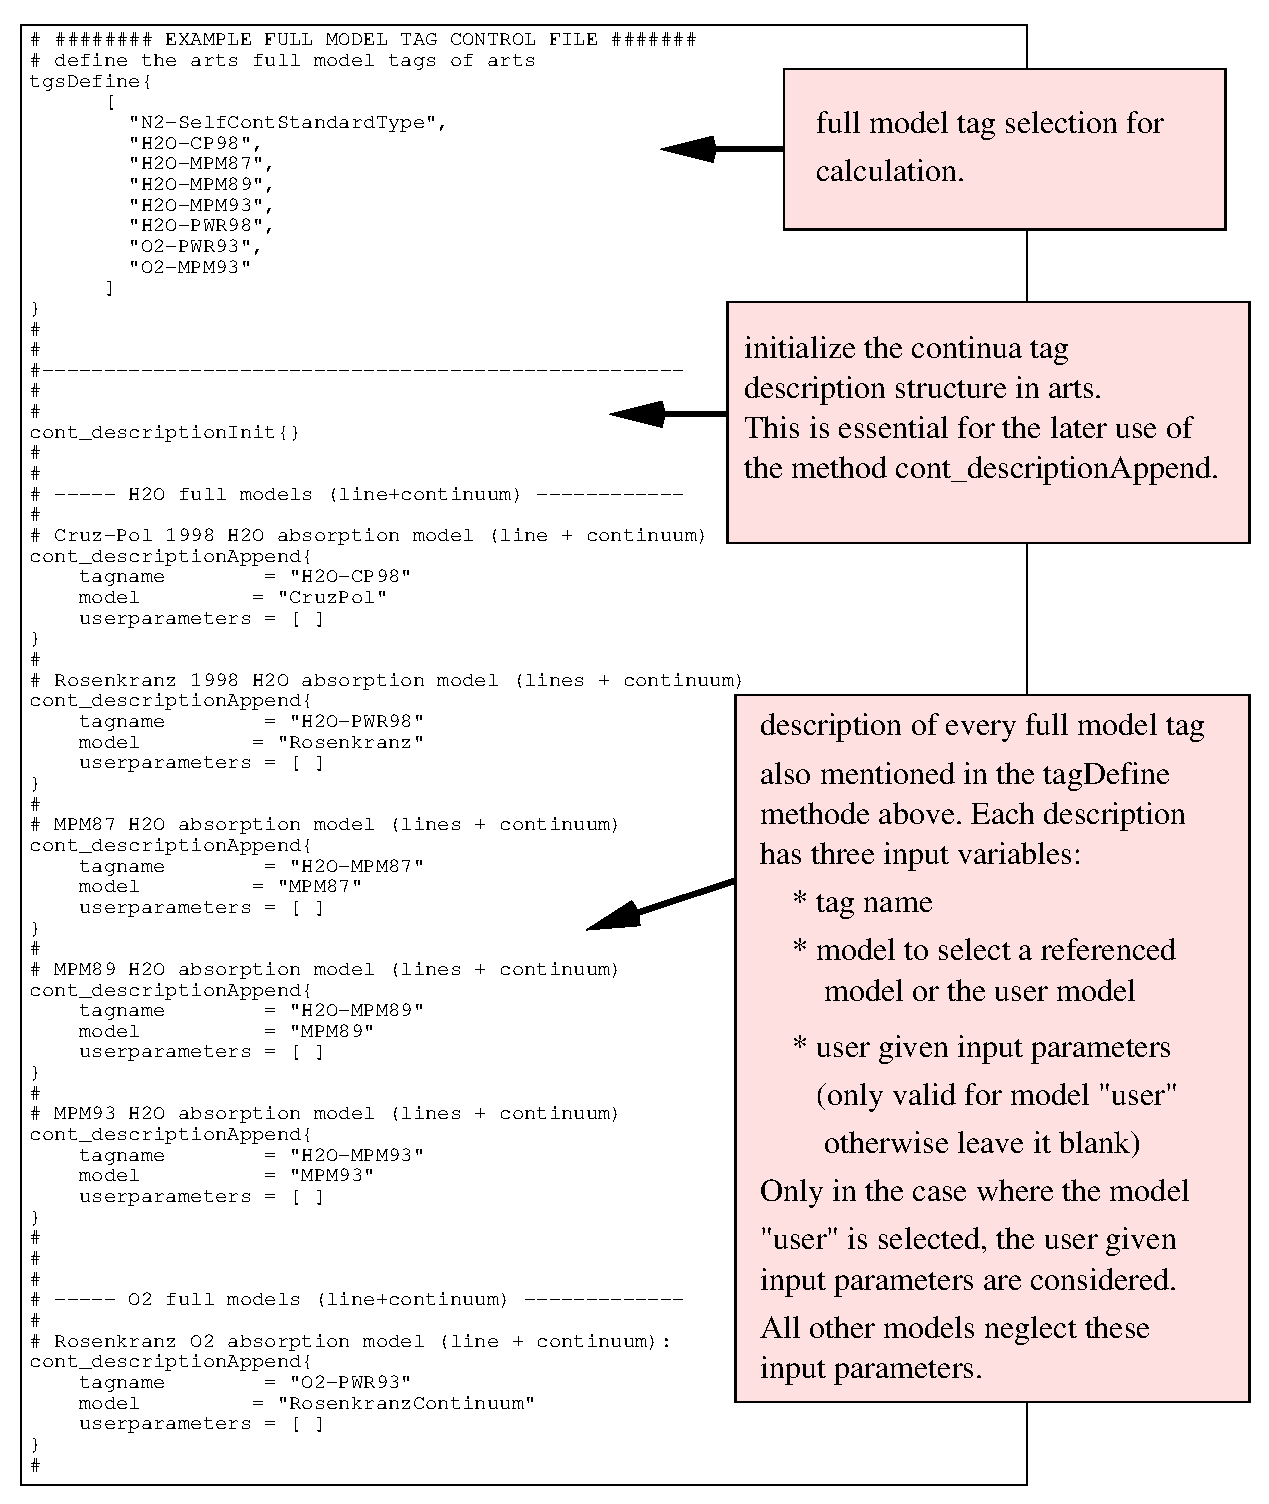
\includegraphics[scale=0.65, angle=0]{fullmodel_description_page1}
\end{flushleft}
\begin{flushleft}
 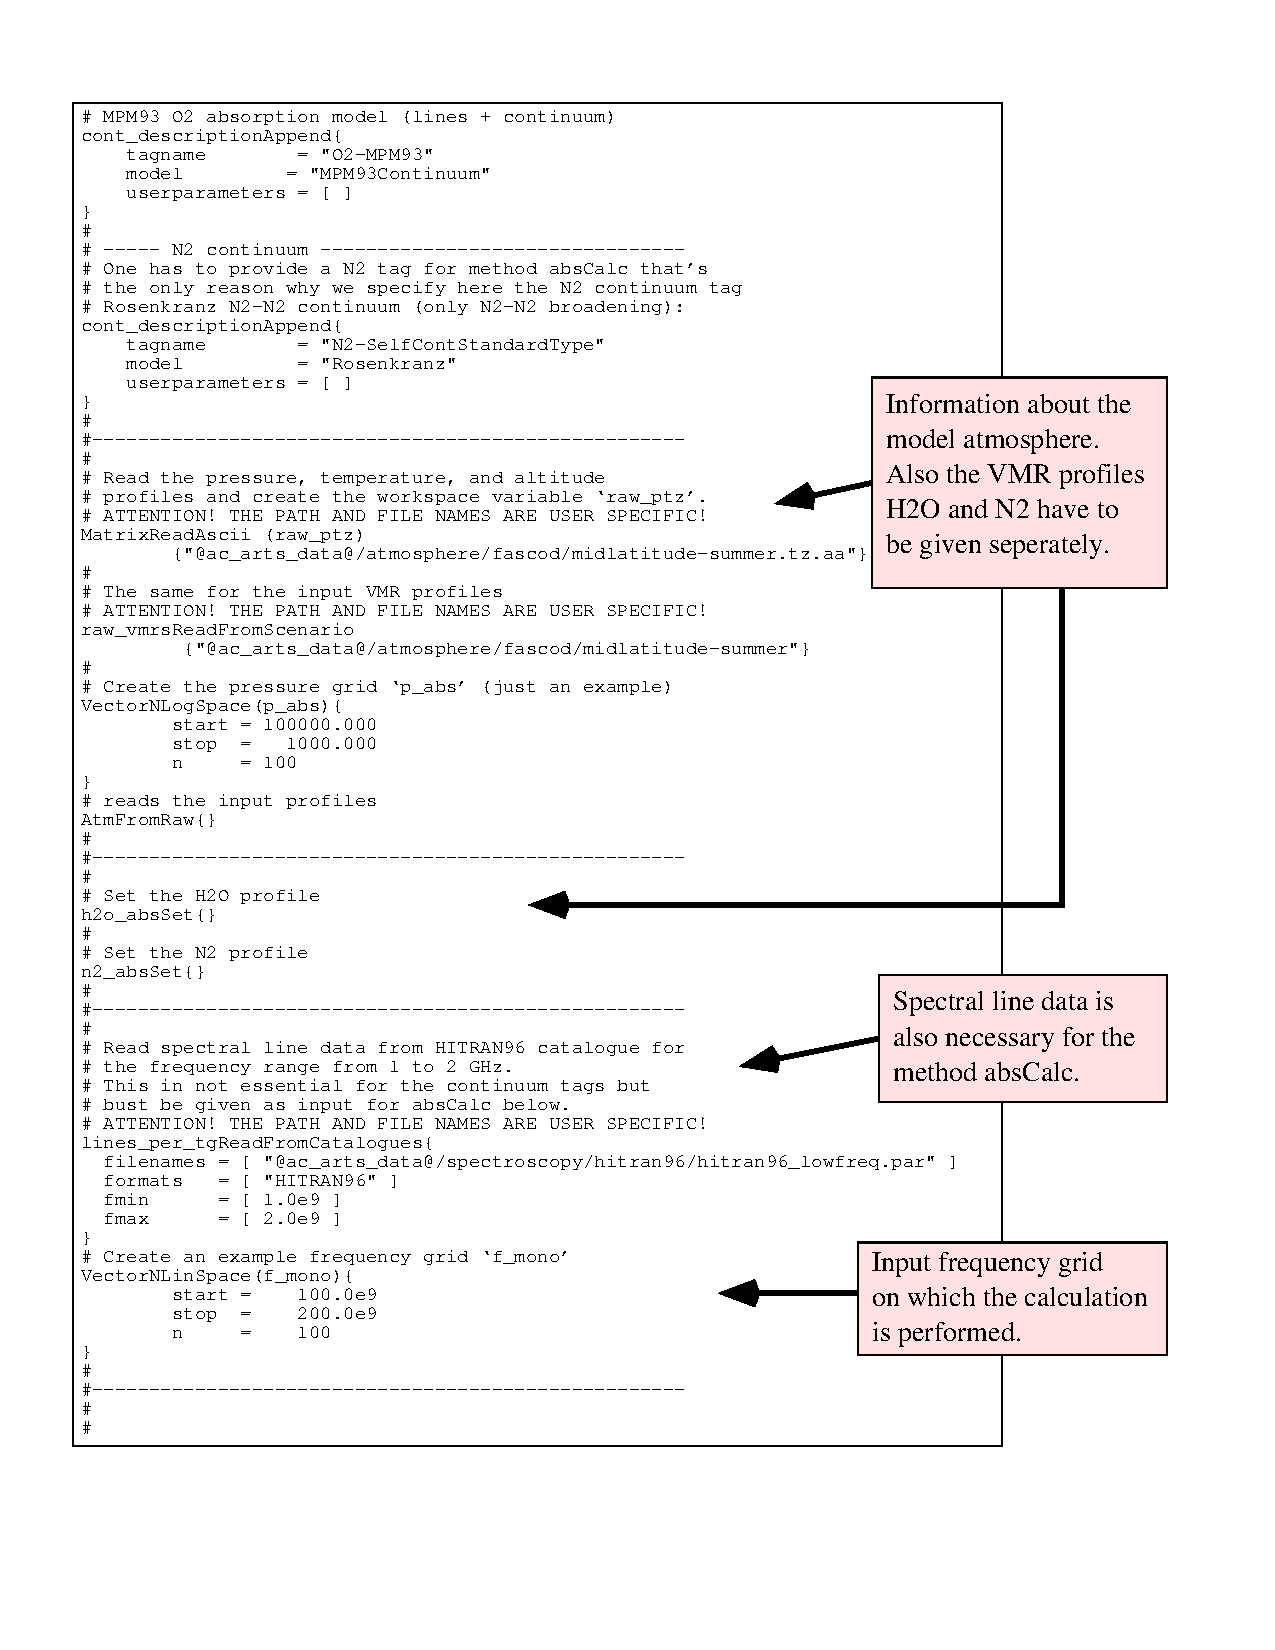
\includegraphics[scale=0.65, angle=0]{fullmodel_description_page2}
\end{flushleft}
\begin{flushleft}
 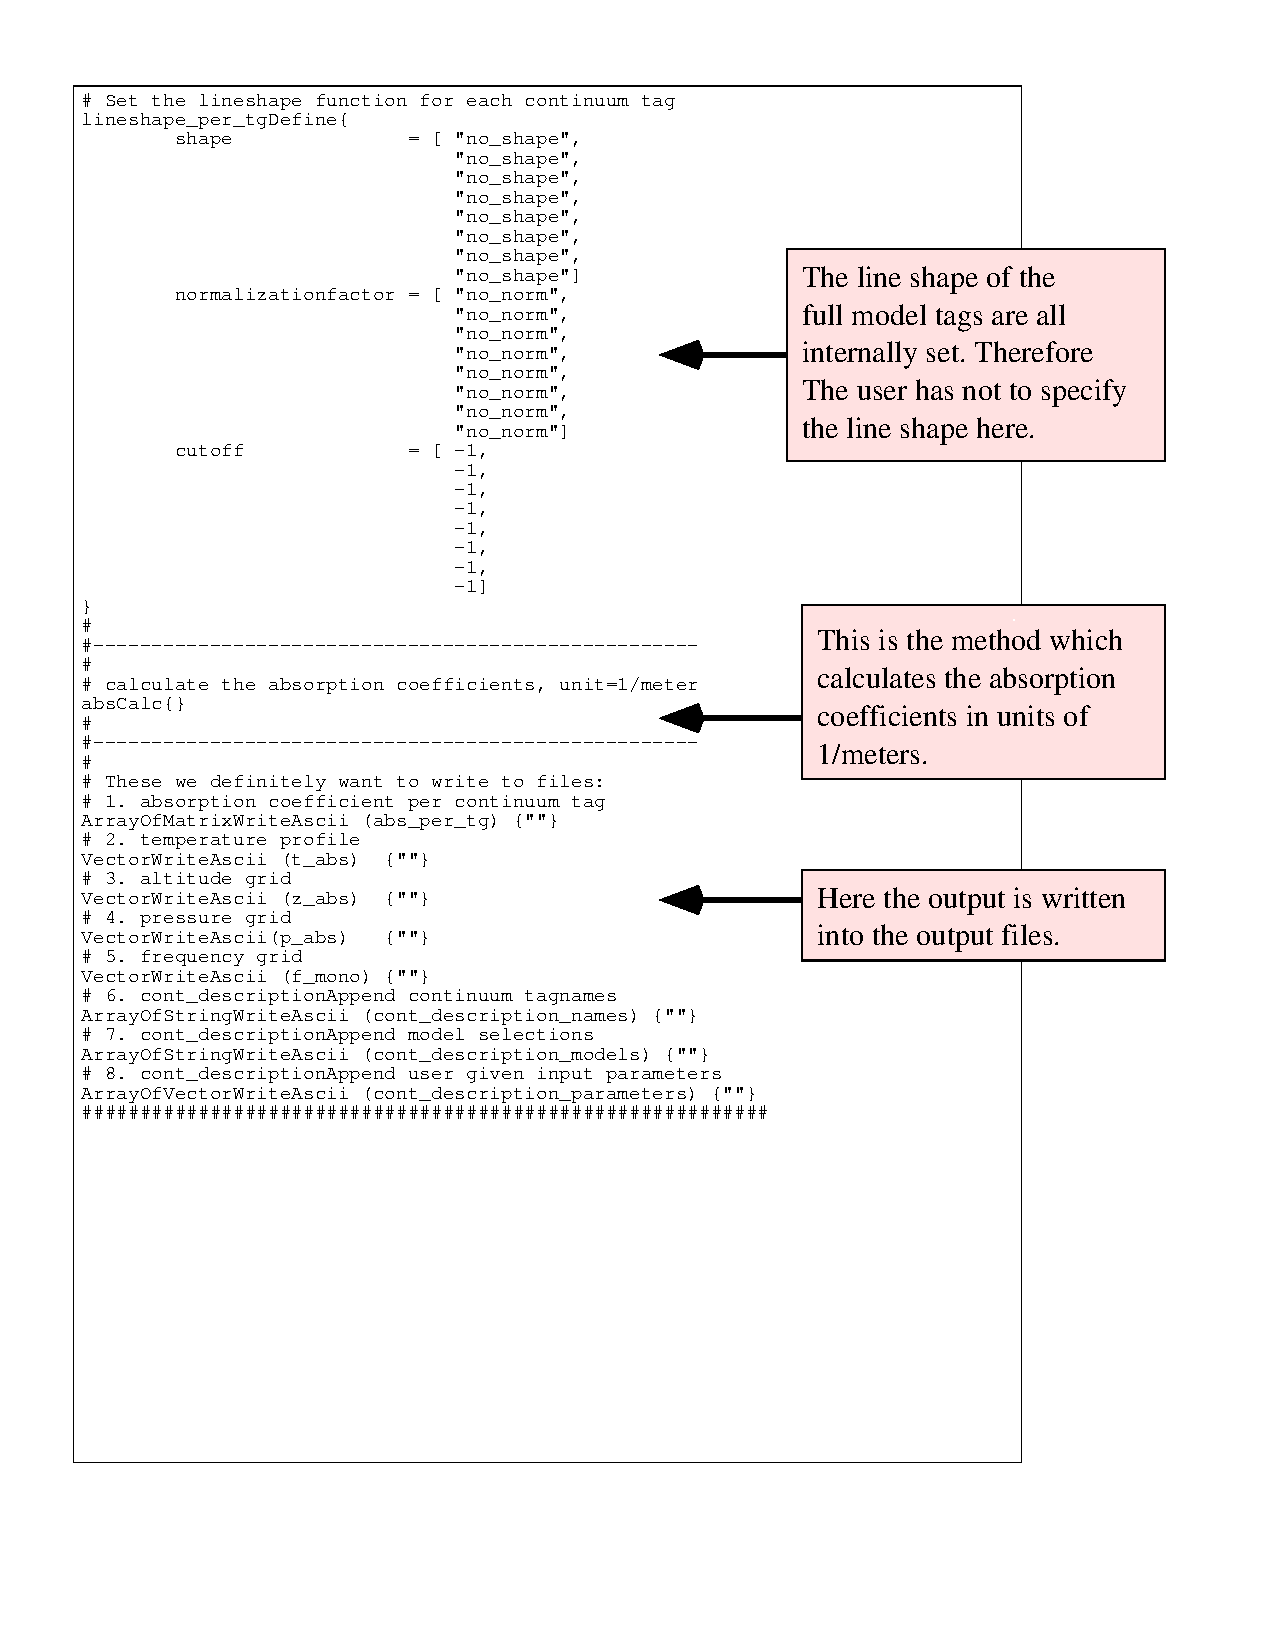
\includegraphics[scale=0.65, angle=0]{fullmodel_description_page3}
\end{flushleft}






%############################################################################# 

% ================================================================================
% The following section is written by Thomas Kuhn, iup Bremen, tkuhn@uni-bremen.de
% ================================================================================

\levela{Cloud Absorption}
\label{labela:cloudabsorption}
%=============================

\levelb{Liquid water and ice particle absorption}
\label{levelb:lipartabs}
%*************************************************
So far only absorption due to air was described. However 
hydrometeors\footnote{We denote liquid water and ice particles, either
  suspended or precipitating, in the air as hydrometeors.}
can have a noticeable effect on the radiative transfer through the
atmosphere in the 10-30\,GHz frequency range.

The MPM93 model provides beside the absorption model of air also an
absorption model for suspended liquid water droplets and ice particles
\citep{liebe:89b,liebeetal:91,hufford:91,liebeetal:93}.  The model is
applicable for the Rayleigh regime, for which the relation $r <
0.05\cdot \lambda$ holds where $r$ is the particle radius and
$\lambda$ is the wavelength\footnote{See \citet{brussaard:95}, page
  81, for details.}, e. g. for a frequency of around 22\,GHz 
this means $r<$~500\,$\mu$m. Considering \citet{salby:96}, this criterium is --
except for cirrus -- nearly for every aerosol and cloud class
satisfied. But one has to bear in mind that these values have a wide
range of variability, for example, \citet{salby:96} states that the
mean particle radius for stratus, cumulus, and nimbus clouds can be in
the range of 10-1000\,$\mu$m and that the particle radius distribution
is highly unsymmetric. 

With respect to the imaginary part of the complex refractivity, a 
unified parameterization of liquid and ice particle absorption 
is formulated in MPM93:
\begin{eqnarray}
  \label{eq:abs_cloud}
  \alpha & = & 0.1820 \cdot \nu \cdot\imn\hspace*{20mm}
               \mbox{dB/km}\\
    \imn & = & \frac{3}{2} \cdot \frac{w}{m} \cdot 
               \Im{[(\er-1)/(\er+2)]}\nonumber\\
    \imn & = & \frac{3}{2} \cdot \frac{w}{m} \cdot 
               \left[\frac{3\cdot\ime}{(\ree+2)^2~+~(\ime)^2}\right]\nonumber\\
  \nonumber
\end{eqnarray}
where $w$ is the liquid water (0.0\,$<LWC<$\,5.0\,g/m$^3$) or ice
mass (0.0\,$IWC$\,1.0\,g/m$^3$) content and $m$ is the water 
or ice bulk density ($\denli$=1.0\,g/cm$^3$ and 0.916\,g/cm$^3$, respectively).\\
The difference between liquid water and ice absorption is put in the 
expressions for the complex permittivities (i. e. the relative 
dielectric constant), $\er=\ree+i\cdot\ime$, which depend on frequency
and temperature.

\noindent$\bullet$ Complex permittivity for suspended liquid water droplets:
\begin{eqnarray}
  \label{eq:comp_perm_lwc}
  \ree       & = & \epsilon_o~-~\nu^2\cdot
                   \left[\frac{\epsilon_o-\epsilon_1}{\nu^2+\gamma_1^2}~+~
                   \frac{\epsilon_1-\epsilon_2}{\nu^2+\gamma_2^2}\right]\nonumber\\
%
  \ime       & = & \nu\cdot\left[\gamma_1\cdot
                   \frac{\epsilon_o-\epsilon_1}{\nu^2+\gamma_1^2}~+~
                   \gamma_2\cdot\frac{\epsilon_1-\epsilon_2}{\nu^2+\gamma_2^2}\right]\nonumber\\
%
  \label{eq:comp_perm_lwc_epsilon_0}
  \epsilon_o & = & 77.66 + 103.3\cdot(\Theta-1)\\
  \epsilon_1 & = & 0.0671\cdot\epsilon_o\nonumber\\
  \epsilon_2 & = & 3.52\nonumber\\
%
  \label{eq:comp_perm_lwc_gamma_1}
  \gamma_1   & = & 20.20 - 146\cdot(\Theta-1) + 316\cdot(\Theta-1)^2\,\mbox{GHz}\\
  \gamma_2   & = & 39.8\cdot\gamma_1\,\mbox{GHz}\nonumber\\
%
  \Theta     & = & 300\,\mbox{K}~/~T\nonumber
%
%  LWC        & = & 0.0~\mbox{to}~5.0~\mbox{g}/\mbox{m}^3
%                   \hspace*{10mm}\mbox{cloud liquid water content}\nonumber\\
%  \rho_l     & = & 1.0~\mbox{g}/\mbox{cm}^3
%                \hspace*{10mm}\mbox{water density}\nonumber
%  \nonumber
\end{eqnarray}
$\bullet$ Complex permittivity for ice crystals:
\begin{eqnarray}
  \label{eq:comp_perm_iwc}
  \ree    & = & 3.15\nonumber\\
%
  \ime    & = & \frac{a}{\nu}~+~b\cdot\nu\nonumber\\
%
  \label{eq:comp_perm_iwc_a}
  a       & = & (\Theta-0.1871)\cdot\exp{(17.0-22.1\cdot\Theta)}\\
  \label{eq:comp_perm_iwc_b}
  b       & = & \left[\left(\frac{0.233}{1-0.993/\Theta}\right)^2 + 
                \frac{6.33}{\Theta} - 1.31\right]\cdot10^{-5}\\
%
  \Theta  & = & 300\,\mbox{K}~/~T\nonumber
%
%  IWC     & = & 0.0~\mbox{to}~1.0~\mbox{g}/\mbox{m}^3 
%                \hspace*{10mm}\mbox{cloud ice water content}\nonumber\\
%  \rho_i    & = & 0.916~\mbox{g}/\mbox{cm}^3
%                \hspace*{10mm}\mbox{ice density}\nonumber
%  \nonumber
\end{eqnarray}
%
The absorption is directly proportional to the liquid or ice water
content $LWC/IWC$ and inversely proportional to the density of a
single liquid ice particle $\denli$. Like the mean particle radius,
the liquid and ice water content have a high variability. Table
\ref{tab:lwc} reflects this variability by summarizing different
literature values for several cloud types. Additional uncertainty 
of this absorption term comes from two sides: 
(1) the difference to the Rayleigh approximation
of the order of 1-6\% as reported in \citet{lietal:97} and (2) from
the fit of the complex permittivity.  Since $\epsilon(\nu,T)$ was
fitted to measurements which were mostly performed above $0^\circ$C,
the extrapolated values for $T<$0$^{\rm o}$C for super-cooled
clouds are not well established. For example in \cite{liebeetal:91} 
itself two different parameterizations for the so called primary 
relaxation frequency ($\gamma_1$ in Equation \ref{eq:comp_perm_lwc}) 
are given, one polynomial in $\Theta$ as presented in 
Equation \ref{eq:comp_perm_lwc}) and an exponential function derived
from theory. Although the polynomial describes the selected 
data better than the exponential function, this might not be true for
temperatures well below 0$^{\rm o}$C.
The difference in $\gamma_1$ according to these two approaches can 
be more than 2\,GHz for very low temperatures \citep{liptonetal:99}. 
The resulting consequences from this discrepancy for the absorption 
calculation at three microwave frequencies are shown in 
Figure \ref{fig:refrac_water_comp}. A more detailed
discussion about this source of uncertainty is given in Section
\ref{levelb:ref_uncert_clouds}.
%
\begin{table}[!htb]
\begin{center}
\begin{tabular}{llll}
\hline
\multicolumn{4}{c}{liquid water content ($LWC$)} \\
 cloud        & class & \multicolumn{1}{c}{(g/m$^3$)} & reference\\
\hline
 stratus      & St    & 0.15        & \cite{salby:96}\\
              &       & 0.09-0.9    & \cite{seinfeld:98}\\
              &       & 0.28-0.3    & \cite{hess:98}\\
              &       & 0.29        & \cite{abreu:96}\\
 nimbostratus & Ns    & 0.4         & \cite{salby:96}\\
              &       & 0.65        & \cite{abreu:96}\\
              &       & 0.05-0.3    & \cite{berton:00}\\
 altostratus  & As    & $<$0.01-0.2 & \cite{seinfeld:98}\\
              &       & 0.41        & \cite{abreu:96}\\
              &       & 0.1-1       & \cite{berton:00}\\
 stratocumulus& Sc    & 0.3         & \cite{salby:96}\\
              &       & $<$0.1-0.7  & \cite{seinfeld:98}\\
              &       & 0.15        & \cite{abreu:96}\\
              &       & $<$0.5      & \cite{pawlowskaetal:00}\\
              &       & 0.05-1      & \cite{berton:00}\\
 cumulus      & Cu    & 0.5         & \cite{salby:96}\\
              &       & 0.26-0.44   & \cite{hess:98}\\
              &       & 1.00        & \cite{abreu:96}\\
 cumulonimbus & Cb    & 2.5         & \cite{salby:96}\\
              &       & 0.1-2       & \cite{berton:00}\\
 cumulus 
    congestus & Cg    & 0.1-3.2     & \cite{berton:00}\\
FIRE-ACE      & -     & $<$0.7      & \cite{shupeetal:00}\\
\hline
\multicolumn{4}{c}{}  \\
\multicolumn{4}{c}{ice water content ($IWC$)}  \\
 cloud        & class & \multicolumn{1}{c}{(g/m$^3$)} & reference\\
\hline
 cirrus       & Ci    & 0.025                         & \cite{salby:96}\\
              &       & 0.00193-0.0260                & \cite{hess:98}\\
              &       & 3.128$\cdot$10$^{-4}$-0.06405 & \cite{abreu:96}\\ 
              &       & 0.15-0.3                      & \cite{larsenetal:98}\\
              &       & $<$0.1                        & \cite{berton:00}\\
cirrostratus  & Cs    & 0.2                           & \cite{salby:96}\\
              &       & 0.05-2                        & \cite{berton:00}\\
\hline
\end{tabular}
\caption{Stated values for the liquid and ice water content of several 
  cloud classes from different sources.}
\label{tab:lwc}
\end{center}
\end{table}



\levelb{Variability and Uncertainty in Cloud Absorption}
\label{levelb:ref_uncert_clouds}
%--------------------------------------------------------
In the case of clouds three sources of uncertainties can be considered
at first sight: (1) validity of the Rayleigh approximation (2) the 
parameterization of the relative dielectric constants ($\er$) of water 
and ice in the microwave region, and (3) the statistical and
climatological variability of the cloud liquid water and ice content.

As it was stated above (Section \ref{levelb:lipartabs}) the Rayleigh 
approximation is valid for particle sizes $<$~500\,$\mu$m. Figure 
\ref{fig:cloud_part_dist} shows a particle size distribution for water
clouds and ice clouds (cirrus) from the OPAC model \citep{hess:98}. 
According to this model only cirrus clouds will have particles of size
larger than 500\,$\mu$m. Nevertheless one has to keep in mind that the
variability of the particle size can be very high so that at certain 
conditions some cloud types (most probable is the cumulonimbus) 
a non-negligible large particle concentration can occur.

The uncertainty in the relative dielectric constant of water 
(see e.~g. \citet{liptonetal:99}) is largest below the freezing 
temperature, since only a few measurements at -4$^{\rm o}$C 
contributed to the parameterization of $\er$ in \cite{liebeetal:91}, 
which in turn is used in the cloud liquid water absorption model of MPM93. 
Figure \ref{fig:refrac_water_comp} shows a comparison of 
\cite{liebeetal:91} and \cite{ray:72}\footnote{{The calculations
  for this parameterizastion are performed with the computer code}\\{
   of W. Wiscombe, NASA, GSFC}\\
  (ftp://climate.gsfc.nasa.gov/pub/wiscombe/Refrac\_Index/WATER/)
  For the microwave frequency range this program uses the
  \cite{ray:72} temperature parameterization.} parameterizations 
for the temperature dependence of the expression
$\Im{[(\er-1)/(\er+2)]}$, which is in the Rayleigh approximation 
one of the relevant terms in the absorption calculation (see 
Equation \ref{eq:abs_cloud}). Additionally the same calculations with 
the alternative expression of the first  relaxation frequency, 
$\gamma_1$, as stated in Equation~2b of \cite{liebeetal:91} is shown. 
The three versions give comparable results for temperatures warmer 
than 260\,K but show significant  differences for temperatures below 
240\,K. However, an uncertainty estimation of $\Im{[(\er-1)/(\er+2)]}$ 
is due to the lack of measurements not easy, but it will certainly
increase with decreasing temperature.

The largest variability of the involved quantities of cloud absorption
is the liquid and ice water content ($LWC$ and $IWC$) of the clouds 
(see Table \ref{tab:lwc}). Even within a single cloud the $LWC$ ($IWC$) changes
with altitude and the distance from the cloud center as can be seen for
example in Figure 10 of \citet{ludlammason:57} and in the model study
of \citet{costaetal:00}.




\levelb{Water Vapor Saturation Adjustment in the Cloud}
\label{levelb:WV_sat_in_cloud}
%--------------------------------------------------------

The arts method {\tt WaterVaporSaturationInClouds{}} assures that 
the water vapor partial pressure is automatically set to 
saturation pressure (100\,\% relative humidity) in the cloud vertical
range.
This method sets the water vapor partial pressure to the 
saturation pressure over liquid water in case where liquid clouds 
are present and to the saturation pressure over ice where 
ice or water/ice clouds are present. The calculation of the 
saturation pressure is calculated according to the 
Goff-Gratch approximation \citep{liebeetal:93}:

\begin{eqnarray}
  \theta &=& (373.16\,\mbox{K} / T) \\
%
  x      &=& A \cdot \left(\theta -1 \right) + 
             B \cdot \log{(\theta)} + \nonumber\\ 
         &&  C \cdot \left( 10^{d\cdot (1- \theta^{-1})} -1 \right) +  
             E \cdot \left( 10^{g\cdot (\theta-1)} -1 \right) \\ 
%
  e^w_s  &=& 101324.6 \cdot 10.0^x\,\mbox{Pa} 
\end{eqnarray}
with
\begin{eqnarray}
 A &=& -7.90298 \nonumber \\
 B &=& 5.02808  \nonumber \\
 C &=& -1.3816 \cdot 10^{-7} \nonumber \\
 d &=& 11.344 \nonumber \\
 E &=& 8.1328 \cdot 10^{-3} \nonumber \\
 g &=& -3.49149 \nonumber
\end{eqnarray}


The $\hzo$ saturation pressure over ice the Goff-Gratch 
approximation \citep{liebeetal:93} is as follows:
\begin{eqnarray}
  \theta &=& (273.16\,\mbox{K} / T) \\
%
  x      &=& A \cdot \left(\theta -1 \right) + 
             B \cdot \log{(\theta)} + 
             C \cdot \left( 1- \theta^{-1} \right) \\ 
%
  e^i_s  &=& 610.71 \cdot 10.0^x\,\mbox{Pa} 
\end{eqnarray}
with
\begin{eqnarray}
 A &=& -9.09718  \nonumber \\
 B &=& -3.56654  \nonumber \\
 C &=&  0.876793 \nonumber
\end{eqnarray}



\begin{figure}[!htb]
  \begin{center}
% ---- uncertainty -------------------------------------
%   \includegraphics*[scale=0.6, angle=90, viewport= 80 725 480 70]%
   \includegraphics*[width=0.6\hsize, angle=90]%
   {LWCcloud}\\
% ---- ratio -------------------------------------------
%   \includegraphics*[scale=0.6, angle=90, viewport= 80 725 480 66]%
   \includegraphics*[width=0.6\hsize, angle=90]%
   {IWCcloud}
% ------------------------------------------------------
  \end{center}
  \caption{Cloud particle size distributions according to 
    Equations~3a and 3c and the microphysical properties are from the 
    Tables 1a and 1b of the OPAC model \cite{hess:98}. 
    For the liquid water clouds (upper plot) a modified gamma 
    distribution is assumed whereas for the ice clouds (lower plot) 
    exponential functions are taken.}
  \label{fig:cloud_part_dist}
\end{figure}
%
%
\begin{figure}[!hbt]
  \begin{center}
% ---- comparison --------------------------------------
   \includegraphics*[width=0.75\hsize, angle=0]%
   {refractive_water_comp_T}
% ------------------------------------------------------
  \end{center}
  \caption{Comparison of the imaginary part of the expression 
    \mbox{$(\er-1)/(\er+2)$} for liquid water at the three 
    frequencies of 32.9, 22.6, and 10,3 GHz. Plotted are the two common
    models of \cite{liebeetal:91} (a) and \cite{ray:72} (b). 
    The Ray parameterization is calculated with the F77 program 
    of W. Wiscombe, NASA, GSFC, take from 
    ftp://climate.gsfc.nasa.gov/pub/wiscombe/Refrac\_Index/WATER/.
    Additionally the \cite{liebeetal:91} parameterization (c) with the 
    alternative expression for the first relaxation frequency, 
    $\gamma_1 = 20.1\cdot\exp{[7.88\cdot(1-\Theta)]}$, is plotted.}
%
%    $(\er-1)/(\er+2)$ for liquid water at the three WATS frequencies
%    of interest. Plotted are the two common
%    models of \cite{liebeetal:91} and \cite{ray:72} (calculated with 
%    the F77 program of W. Wiscombe (NASA, GSFC) take from 
%    ftp://climate.gsfc.nasa.gov/pub/wiscombe/Refrac\_Index/WATER/).}
  \label{fig:refrac_water_comp}
\end{figure}




\levelb{ARTS Workspace Variables and Methods}
\label{levelb:ArtsImplementationCloudAbsorption}
% ----------------------------------------------

This section explains how the above described cloud absorption models
are represented in the structure of the arts source code and how 
one can invoke them in the arts control file.

The cloud tags needs not necessarily more input information than 
normal trace gas tags, since both need only a profile. But to have 
more flexibility one can run these absorption models as black boxes 
or with some user given input. In connection with this input parameters 
we distinguish generally two types, the referenced models which 
are taken from the literature (e. g. \cite{liebeetal:93}) and the 
user model, for which the arts user is providing the necessary 
parameter values.

Formally the cloud tags are like the 
continuum or full model tags implemented. Therefore after selecting 
the cloud tag with the {\tt tagDefine} method, the arts user has to 
setup the arts internal structure (i. e. the workspace variables 
{\it cont\_description\_names, cont\_description\_models, 
and cont\_description\_parameters}) for the selected continuum tags, 
which can simply be done by putting the following line into the 
arts control file:
\begin{verbatim}
cont_descriptionInit{}
\end{verbatim}

After this initialization, the cloud tag specific
information has to be transfered to arts. This is possible with the 
arts method {\it cont\_descriptionAppend}, which has itself 
three input variables: {\it tagname}, {\it model}, and 
{\it userparameters}. The user has to specify these input 
variables in the arts control file for each selected cloud tag. 
Below is a list of all the implemented continuum tags and the associated
valid range of the input variables for {\it cont\_descriptionAppend}. 
For an overview of the possible continuum tags and their 
referenced models see Table \ref{tab:artscloudlist} and the 
online documentation can be found under 
{\it arts/doc/doxygen/html/continua\_cc.html}.

One has to note at this place that the two input variables {\it model} and
{\it userparameters} are to some extend redundant. Therefore one can also 
produce an ambiguity by giving contradicting values for these two input variables.
To avoid such ambiguities the arts user should keep in mind the general 
rule that only the user model ({\it model ="user"}) needs input parameters 
via the input variable {\it userparameters}. The referenced models 
need no input via {\it userparameters}. If you try to run the arts control 
file with a referenced model and input parameters you will get an error message.
Below in the detailed description of {\it cont\_descriptionAppend} you 
can find correct examples for all the cloud tags.

\begin{itemize}
\item[$\bullet$] The liquid water cloud absorption model of 
     MPM93 \citep{liebeetal:93} has the arts tag name 
     {\tt "liquidcloud-MPM93"}. The details about this 
     absorption model are described in Section 
     \ref{labela:cloudabsorption}. The standard way to use 
     the MPM93 liquid water cloud absorption model is to set 
     the input variable {\it model} to "MPM93" and leaving 
     the input parameter {\it userparameters} empty. \\ To 
     have a minimum possibility of variation one can also run 
     this tag with {\it model}\,=\,"user". In this case one 
     has to provide three input parameters via {\it userparameters}, 
     e. g. {\it userparameters}\,=\,$[CC$, $CG$, $CE]$. The first 
     input parameter ($CC$) scales the total liquid water cloud absorption 
     (see Eq. \ref{eq:abs_cloud}) while $CG$ scales the first 
     relaxation frequency, $\gamma_1$, (see Eq. 
     (\ref{eq:comp_perm_lwc_gamma_1})) and  $CE$ scales $\epsilon_o$ 
     (see Eq. \ref{eq:comp_perm_lwc_epsilon_0})
\begin{verbatim}
cont_descriptionAppend{
    tagname        = "liquidcloud-MPM93"
    model          = "MPM93"
    userparameters = [ ]
}
cont_descriptionAppend{
    tagname        = "liquidcloud-MPM93"
    model          = "user"
    userparameters = [ 1.0, 1.0, 1.0 ]
}
\end{verbatim}
\item[$\bullet$] The ice water cloud absorption model of 
     MPM93 \citep{liebeetal:93} has the arts tag name 
     {\tt "icecloud-MPM93"}. The details about this 
     absorption model are described in Section 
     \ref{labela:cloudabsorption}. The standard way to use 
     the MPM93 ice water cloud absorption model is to set 
     the input variable {\it model} to "MPM93" and leaving 
     the input parameter {\it userparameters} empty. \\ To 
     have a minimum possibility of variation one can also run 
     this tag with {\it model}\,=\,"user". In this case one 
     has to provide three input parameters via {\it userparameters}, 
     e. g. {\it userparameters}\,=\,$[CC$, $CA$, $CB]$. The first 
     input parameter ($CC$) scales the total ice water cloud absorption 
     (see Eq. \ref{eq:abs_cloud}) while $CA$ scales $a$, (see Eq. 
     (\ref{eq:comp_perm_iwc_a})) and $CB$ scales $b$ 
     (see Eq. \ref{eq:comp_perm_iwc_b})
\begin{verbatim}
# MPM93 model for ice water particle absorption:
cont_descriptionAppend{
    tagname        = "icecloud-MPM93"
    model          = "MPM93"
    userparameters = [ ]
}
# MPM93 model for ice water particle absorption:
cont_descriptionAppend{
    tagname        = "icecloud-MPM93"
    model          = "user"
    userparameters = [ 1.0, 1.0, 1.0 ]
}
\end{verbatim}
\end{itemize}


Another important point is to state in the arts control file which
cloud profile should be read in. Becasue for a single climate zone one
can have several different cloud types, it is not enough to state 
e. g. just {\it midlatitude-summer} or {\it tropical} as for 
trace gases. Therefore the method {\tt raw\_vmrsReadFromFiles} has to 
be used to read in the trace gas and clooud profiles. For example 
the following lines in the control file will read in trace gas 
profiles from a midlatitude-summer scenario (this information is
provided with the input variable {\it basename} which states the 
basic scenario) and cumulonimbus and cirrus cloud profiles for 
liquid water and ice water clouds, respectively:
\begin{verbatim}
# ATTENTION! THE PATH AND FILE NAMES ARE USER SPECIFIC!
raw_vmrsReadFromFiles
  {seltags   = [ "liquidcloud-MPM93", 
                 "icecloud-MPM93" ]
   filenames = [ "cumulonimbus.MPM93droplet.aa",
                 "cirrus.MPM93ice.aa" ]
   basename  =   "midlatitude-summer"
  }
#
\end{verbatim}
The method {\tt raw\_vmrsReadFromFiles}can be used for any tag and 
is not specific for cloud tags. In general one has to state in the 
input variable {\it seltags} the tags which take their profile 
information from the files stated in the input variable 
{\it filenames}, while all the tags which are not stated in 
{\it seltags} take their profile information, i. e. the atmospheric 
scenario, from the input variable {\it basename}. 

To set the water vapor pressure in the cloud range to the saturation 
pressure you can use the method {\tt WaterVaporSaturationInClouds{}}
after the call of the method {\tt AtmFromRaw{}}. The saturation
pressure is calculated over liquid water in liquid water clouds and
over ice in ice water clouds. If both cloud types are present the
saturation over ice is taken.

\begin{landscape}
 \setlength{\LTcapwidth}{180mm} % with of the caption in longtable
 \begin{longtable}{llllll}
 K & K & K & K & K & K \kill
%
% --------------------- only begin of table ------------------------------
 \hline
 continuum & \multicolumn{3}{c}{{\it cont\_descriptionAppend} input} & 
 reference/ & arts source code function\\
 & \multicolumn{3}{c}{input parameter} & arts uguide & \\
 \hline
 \endfirsthead
% --------------------- every page begin of table ------------------------
 \hline
 continuum & \multicolumn{3}{c}{{\it cont\_descriptionAppend}} & 
 reference/ & arts source code function\\
 & \multicolumn{3}{c}{input parameter} & arts uguide & \\
 \hline
 \endhead
% --------------------- every page end of table ------------------------
 K & K & K & K & K & K \kill
 \hline
 \caption[]{(continued)}\\
 \endfoot
% --------------------- only end of table ------------------------------
 K & K & K & K & K & K \kill 
 \hline
 \caption{This table gives an overview of the implemented referenced 
   cloud absorption models and how they are specified 
   in the arts method {\it cont\_descriptionAppend}. Additionally the 
   reference and the arts source code function names (see file 
   {\it arts/src/continua.cc} are provided. The detailed online 
   documentation can be found under 
   {\it arts/doc/doxygen/html/continua\_cc.html}).}
 \label{tab:artscloudlist}
 \endlastfoot
% --------------------- body of table  ----------------------------------  
 \multicolumn{6}{c}{{\bf water vapor ($\hzo$)}}\\
 \hline
% --------------------------------------------------------------
 MPM93       & tagname &=& {\tt "liquidcloud-MPM93"} & \cite{liebeetal:93} & 
             MPM93WaterDropletAbs\\
             & model   &=& "MPM93"    &   &  \\ 
             & userparameters &=& [ ] &   & \\
 \hline
% --------------------------------------------------------------
 MPM93       & tagname &=& {\tt "icecloud-MPM93"} & \cite{liebeetal:93} & 
               MPM93IceCrystalAbs\\
             & model   &=& "MPM93"    &   &  \\ 
             & userparameters &=& [ ] &   & \\
 \hline
% -----------------------------------------------------------------------  
 \end{longtable}
 \setlength{\LTcapwidth}{0.8\textwidth}
\end{landscape}




\leveld{ARTS Example Control File for the Full Model Tags}
\label{leveld:ArtsCloudModelExampleControlFile}
% --------------------------------------------------------
Below you will find an example of a control file for all 
the implemented cloud absorption models. At the moment only 
the MPM93 model for water and ice clouds is implemented.
Please note that to run this example control file you 
have to specify user specific paths and input file names 
to run it properly. You can find this example in the 
arts directory {\it arts/doc/examples/cloud\_example.arts}
%
\begin{flushleft}
 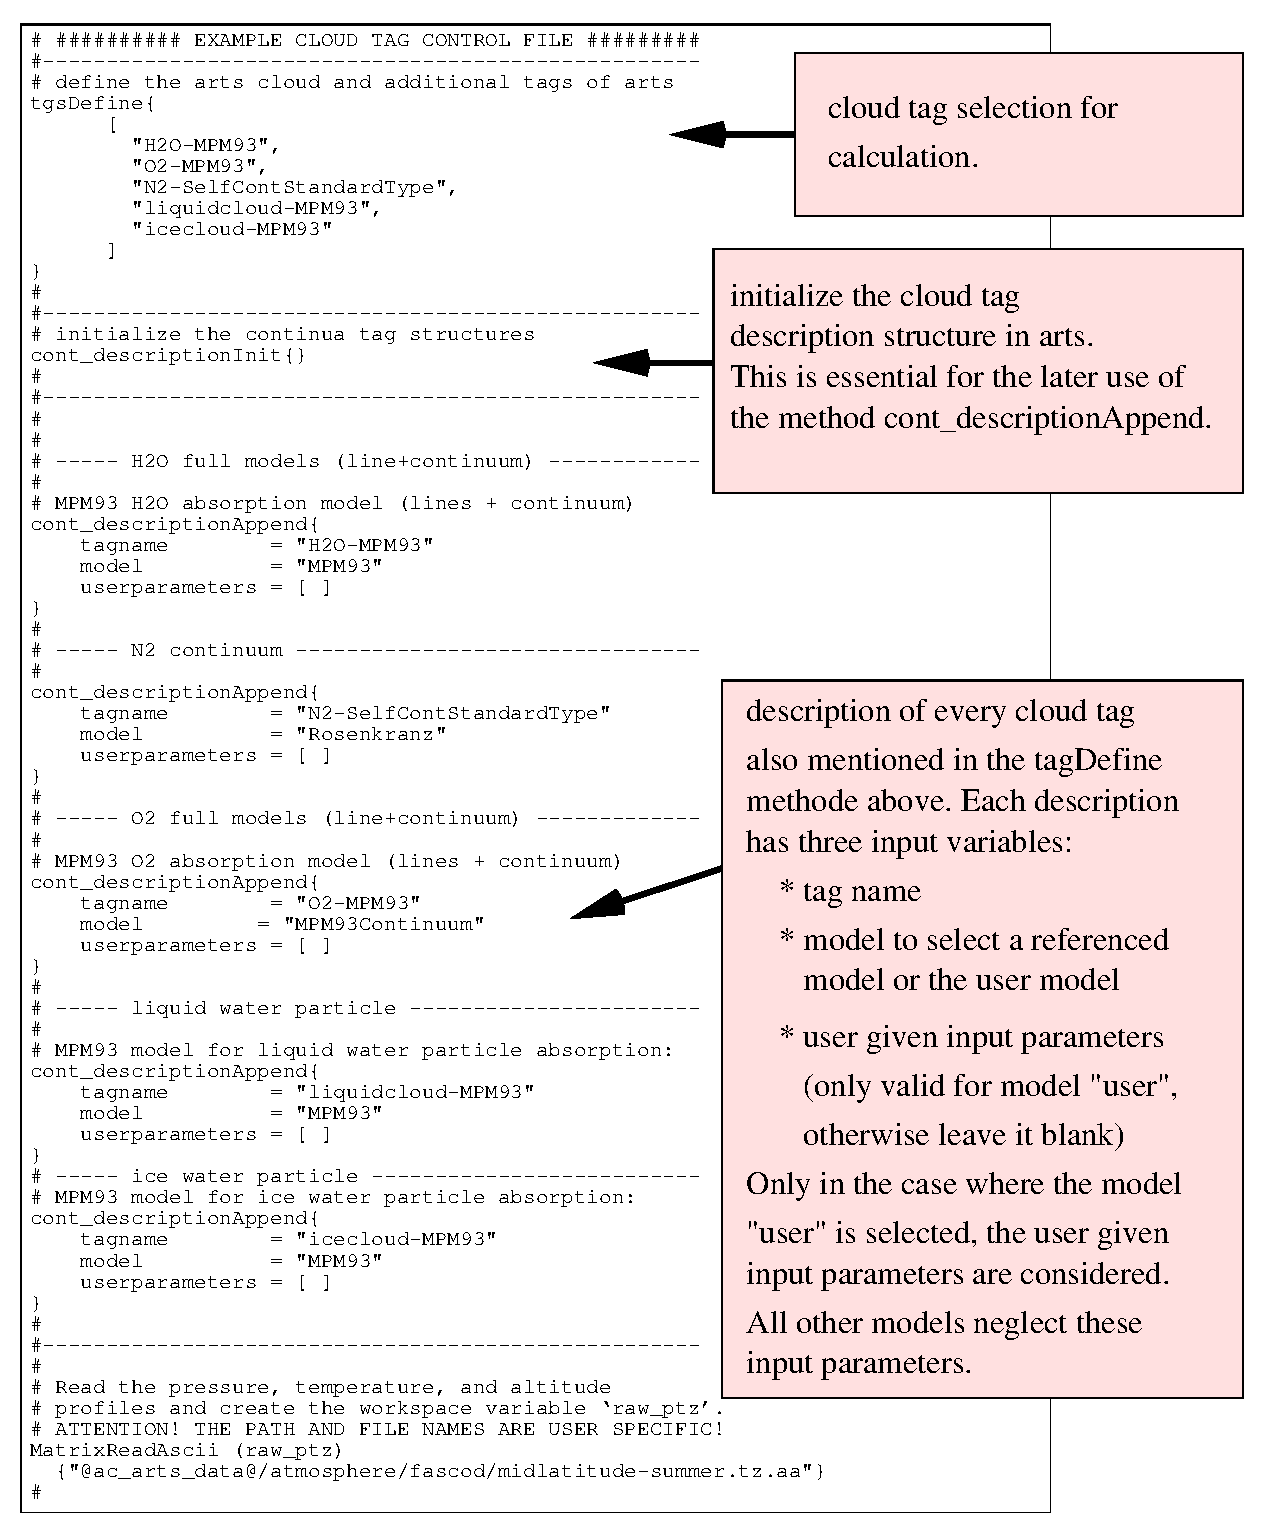
\includegraphics[scale=0.65, angle=0]{cloud_description_page1}
\end{flushleft}
\begin{flushleft}
 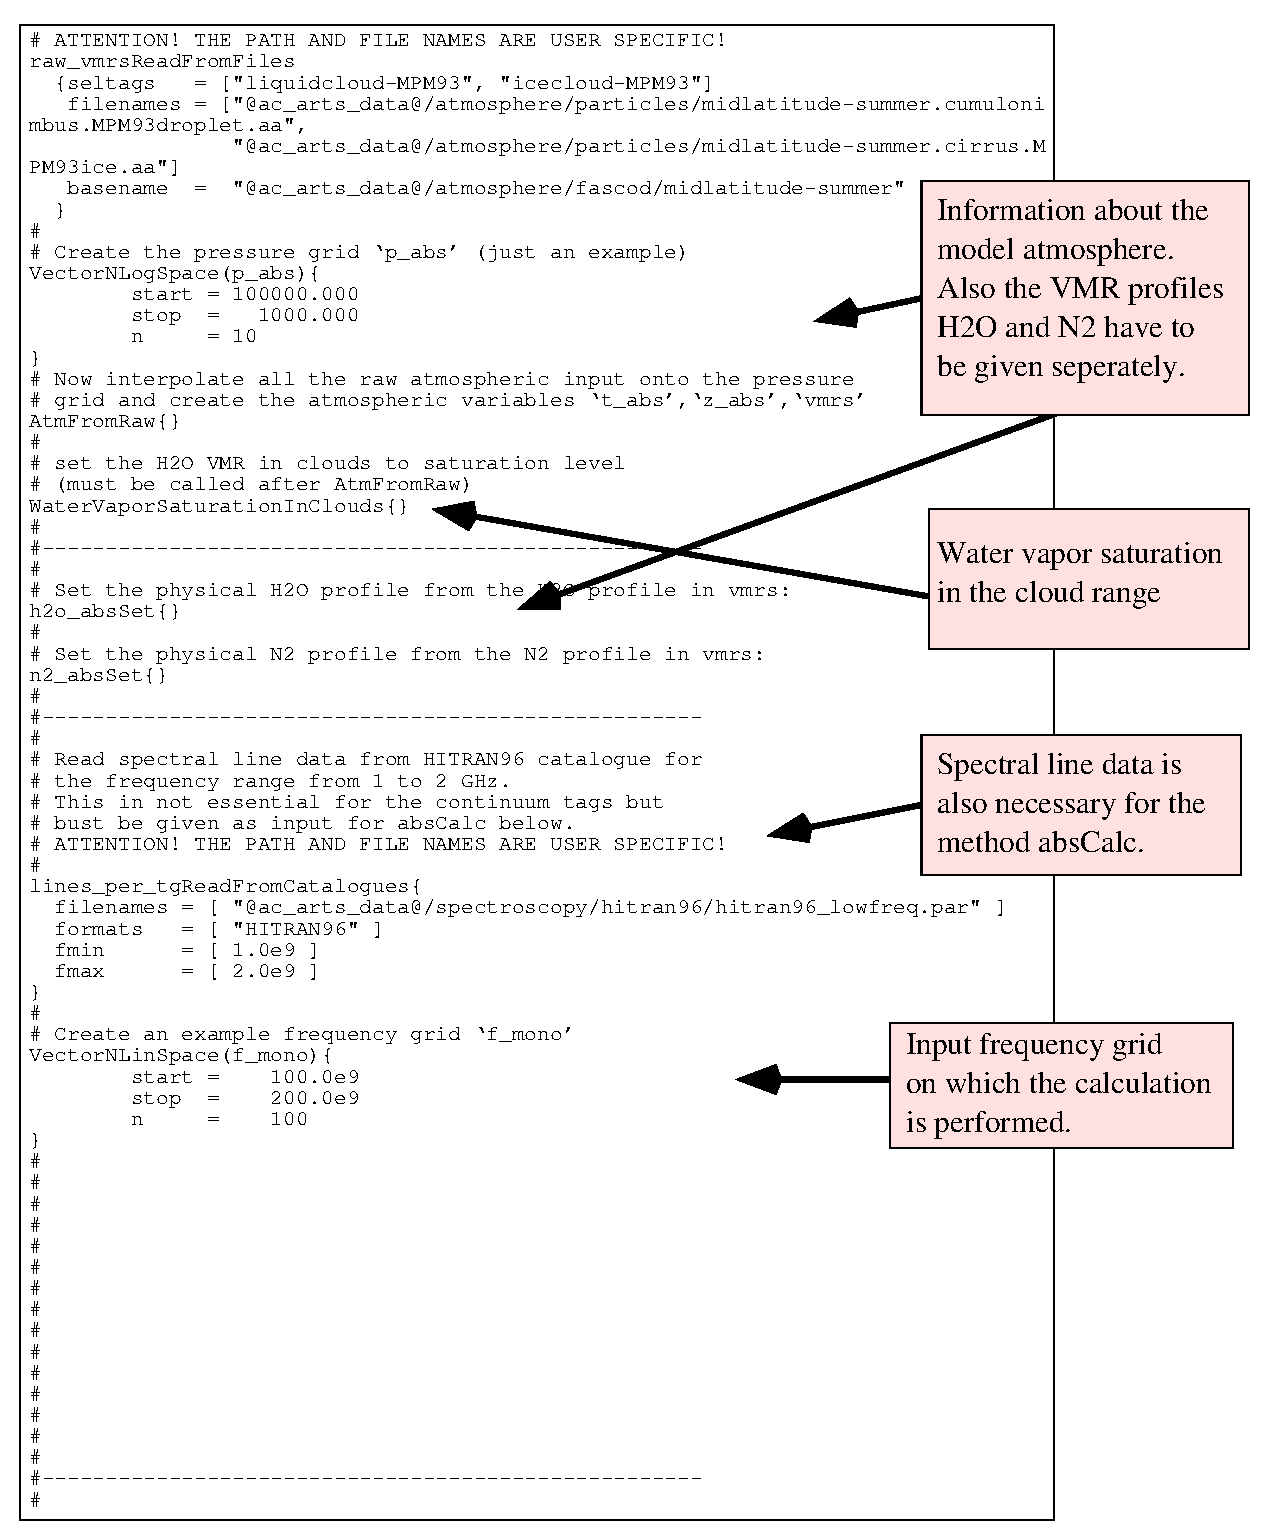
\includegraphics[scale=0.65, angle=0]{cloud_description_page2}
\end{flushleft}
\begin{flushleft}
 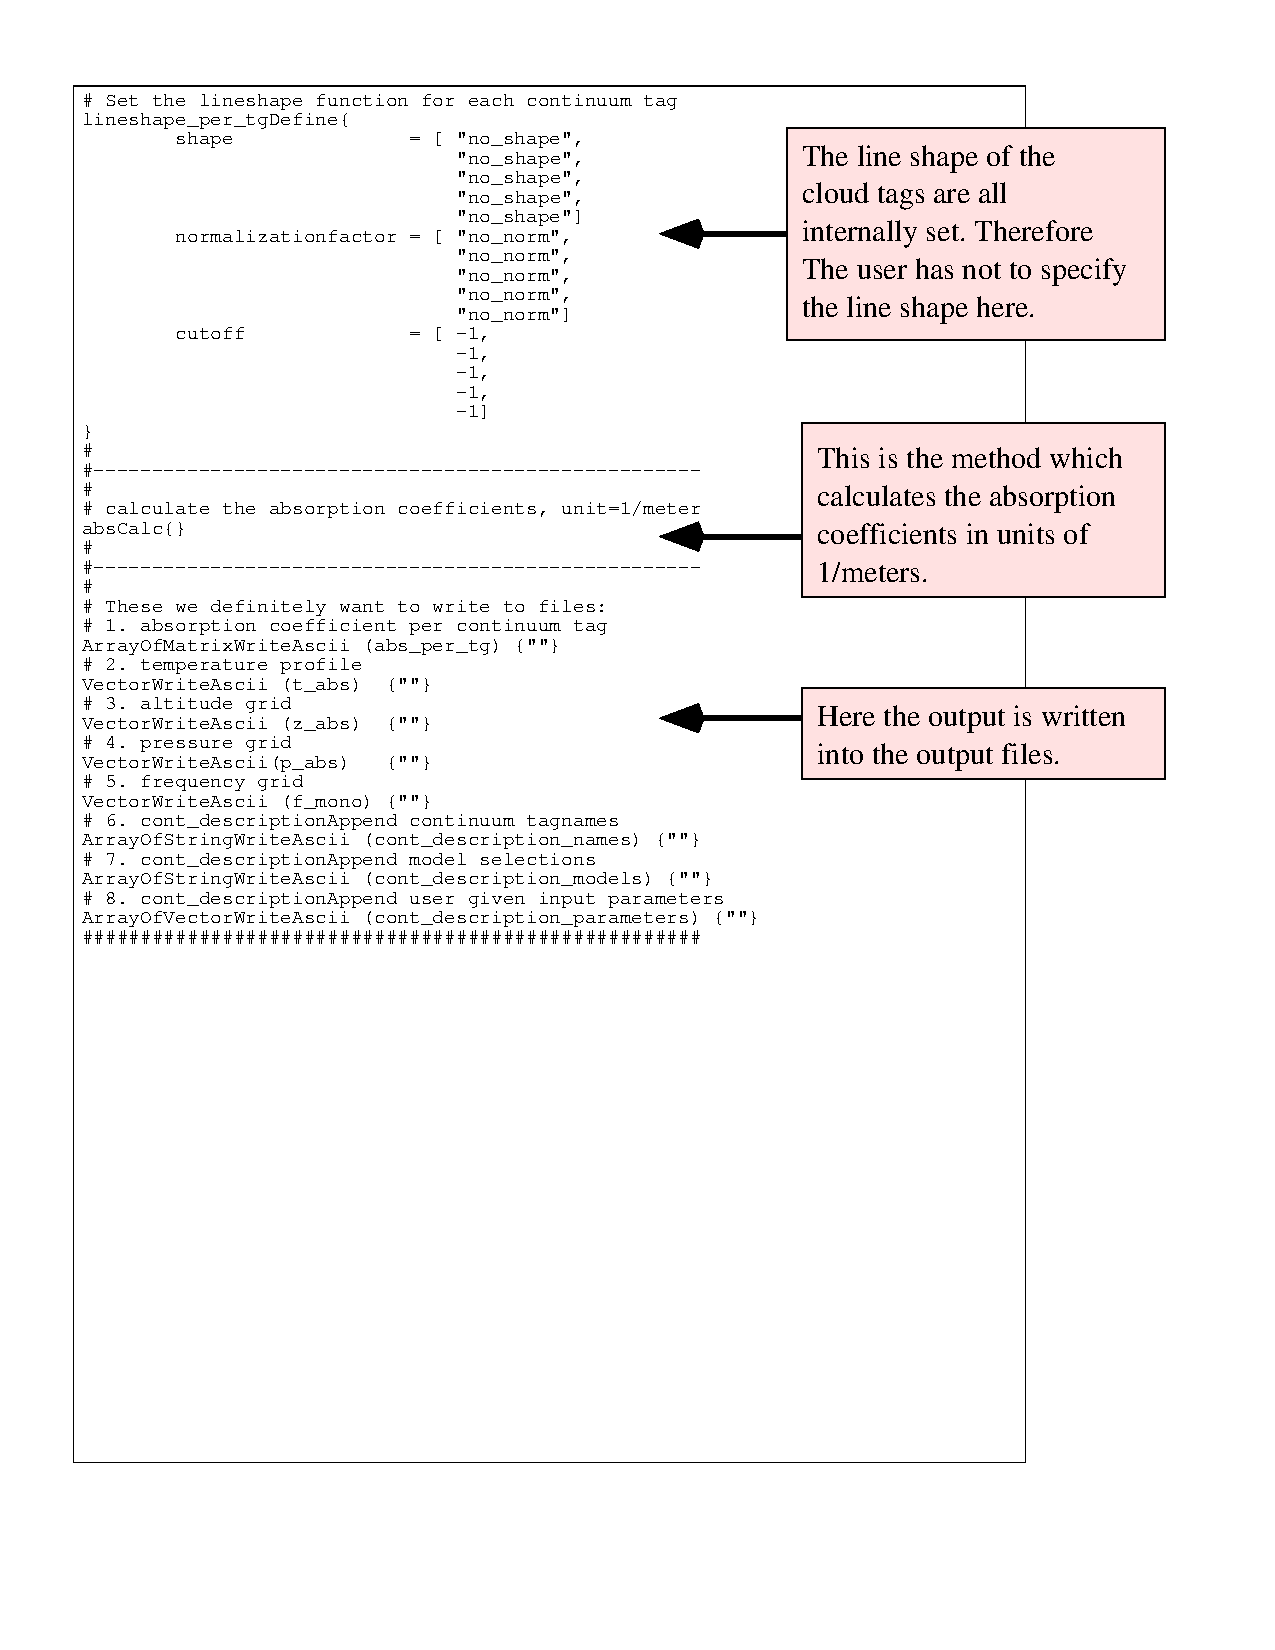
\includegraphics[scale=0.65, angle=0]{cloud_description_page3}
\end{flushleft}



%%% Local Variables: 
%%% mode: latex 
%%% TeX-master: "uguide"
%%% End:

% LocalWords:  Atmosperic
